% ===== BLOQUE: 00_preambulo_REE.tex =====
% ==============================================================================
% DOCUMENTO METODOLÓGICO - CALIBRACIÓN PD->PIT COMPORTAMENTAL PP REENGANCHE (REE)
% Modelo: BetaCal TTC + Vasicek 1-factor PIT + Macro (OLS probit, IPC Lima)
% ==============================================================================
\documentclass[12pt, a4paper]{article}

\usepackage[utf8]{inputenc}
\usepackage[T1]{fontenc}
\usepackage[spanish]{babel}
\usepackage{amsmath, amssymb, amsthm}
\usepackage{graphicx}
\usepackage{booktabs}
\usepackage{longtable}
\usepackage{array}
\usepackage{float}
\usepackage{hyperref}
\hypersetup{hidelinks}
\usepackage{geometry}
\usepackage{fancyhdr}
\usepackage{titlesec}
\usepackage{caption}
\usepackage{xcolor}
\usepackage{enumitem}
\usepackage{setspace}
\usepackage{multirow}
\usepackage{tabularx}
\usepackage{colortbl}

\geometry{left=2.5cm, right=2.5cm, top=3cm, bottom=3cm}
\onehalfspacing

% Tolerancia de composicion: los nombres de tabla/columna/parametro son tokens
% largos en \texttt{} que no admiten guionado.
\setlength{\emergencystretch}{3em}
\tolerance=1500
\hbadness=10000
\vbadness=10000

\graphicspath{{figuras/}{./}}

% --- Colores institucionales (IBK verde) ---
\definecolor{azuloscuro}{RGB}{0,102,51}
\definecolor{azulclaro}{RGB}{0,153,76}
\definecolor{grissuave}{RGB}{240,240,240}
\definecolor{semverde}{RGB}{34,139,34}
\definecolor{semamarillo}{RGB}{218,165,32}
\definecolor{semrojo}{RGB}{178,34,34}

\titleformat{\section}{\Large\bfseries\color{azuloscuro}}{\thesection}{1em}{}
\titleformat{\subsection}{\large\bfseries\color{azulclaro}}{\thesubsection}{1em}{}
\titleformat{\subsubsection}{\normalsize\bfseries}{\thesubsubsection}{1em}{}

\setlength{\headheight}{14pt}
\pagestyle{fancy}
\fancyhf{}
\fancyhead[L]{\small\textcolor{azulclaro}{Calibración PD$\to$PIT --- Comportamental PP Reenganche}}
\fancyhead[R]{\small\textcolor{azulclaro}{Documento Metodológico V1.0}}
\fancyfoot[C]{\thepage}
\renewcommand{\headrulewidth}{0.4pt}

\newcommand{\PD}{\ensuremath{\mathrm{PD}}}
\newcommand{\PDTTC}{\ensuremath{\mathrm{PD}^{\mathrm{TTC}}}}
\newcommand{\PDPIT}{\ensuremath{\mathrm{PD}^{\mathrm{PIT}}}}
\newcommand{\PDraw}{\ensuremath{\mathrm{PD}^{\mathrm{raw}}}}
\newcommand{\RD}{\ensuremath{\mathrm{RD}}}
\newcommand{\LRA}{\ensuremath{\mathrm{LRA}}}
\renewcommand{\rho}{\ensuremath{\varrho}}
\newcommand{\ft}{\ensuremath{f_t}}
\newcommand{\logit}{\ensuremath{\mathrm{logit}}}
\newcommand{\EC}{\ensuremath{\mathrm{EC}}}
\newcommand{\Norm}{\ensuremath{\Phi}}

\newtheorem{definicion}{Definición}[section]

\newenvironment{recuadro}[1]
{\begin{center}\begin{tabular}{|p{0.92\textwidth}|}
\hline
\rowcolor{grissuave}
\textbf{#1} \\ \hline
}
{\\ \hline \end{tabular}\end{center}}

% ==============================================================================

% ===== BLOQUE: 01_portada_REE.tex =====
\begin{document}

\begin{titlepage}
\centering
\vspace*{3cm}
{\Huge\bfseries\textcolor{azuloscuro}{Documento Metodológico}}\\[0.8cm]
{\LARGE\textcolor{azulclaro}{Calibración de la Probabilidad de Default}}\\[0.5cm]
{\Large\textcolor{azulclaro}{Producto: Comportamental --- Préstamo Personal Reenganche (REE)}}\\[2cm]
\rule{0.8\textwidth}{0.5pt}\\[1cm]
{\large
\begin{tabular}{ll}
\textbf{Modelo:}        & Calibración Comportamental PP Reenganche \\
\textbf{Segmentación:}  & \texttt{tipo\_ingreso\_dep}: DEP / NO DEP \\
\textbf{Horizonte:}     & 12 meses (RD12) \\
\textbf{Ventana fit:}   & cohortes maduras 202312--202506 (Z1) \\
\textbf{Proyección:}    & 202507--202512 (método V1) \\
\textbf{Versión:}       & V1.0 \\
\end{tabular}
}\\[2cm]
\rule{0.8\textwidth}{0.5pt}\\[1cm]
{\large Gestión de Modelos --- 2026}
\vfill
\end{titlepage}

\newpage

% ===== BLOQUE: A_intro_REE.tex =====
\section*{Control de Versiones}
\begin{table}[H]
\centering
\small
\begin{tabular}{cccp{7.5cm}}
\toprule
\textbf{Versión} & \textbf{Fecha} & \textbf{Autor} & \textbf{Descripción} \\
\midrule
V1.0 & 2026 & Carlos Acosta & Versión inicial. \\
\bottomrule
\end{tabular}
\end{table}

\newpage
\tableofcontents
\newpage

% ======================================================================
\section{Introducción y Alcance}

\subsection{Objetivo del Documento}
El presente documento expone la metodología de \textbf{calibración} de la Probabilidad de
Default (PD) \textbf{point-in-time} (PIT) del modelo comportamental del producto
\textbf{Préstamo Personal Reenganche} (REE). El objetivo es obtener una \textbf{PD calibrada}:
el proceso transforma la PD del modelo de scoring vigente (\texttt{pd\_comppp\_reen\_itc},
versión v4) ---que captura el \emph{ordenamiento relativo} del riesgo--- en probabilidades
alineadas en \emph{nivel} con la \emph{tasa de default real a 12 meses} y ajustadas por el
ciclo macroeconómico corriente. La brecha de nivel que la calibración cierra está medida: la
$\PDraw$ media sobre la ventana de estimación es \textbf{21{,}1\%} contra una tasa de default
observada de \textbf{3{,}31\%}, de modo que el score ordena pero no mide. El resultado es la
PD-PIT calibrada por segmento, cuyo \textbf{uso} y áreas usuarias se declaran en la
\S\ref{sec:uso} (condición necesaria para juzgar la idoneidad de la calibración). El ancla
central es la \textbf{LRA} (\textit{Long-Run Average}): la tasa de default de largo plazo del
segmento, estimada como la mediana (en escala probit) de la RD12 mensual excluyendo el shock
COVID (202001--202012) y el episodio inflacionario (202207--202306).

La calibración tiene dos capas secuenciales:
\begin{enumerate}[nosep]
  \item \textbf{Calibración TTC} (\textit{Through-The-Cycle}): calibra la PD del score
    (BetaCal de Kull et al., 2017) y ancla su media a la LRA del segmento mediante un
    desplazamiento escalar $\delta$ en escala probit.
  \item \textbf{Transformación PIT} (\textit{Point-In-Time}): convierte la PD~TTC en una PD
    sensible al ciclo mediante el modelo de factor único de Vasicek (2002), con un factor de
    ciclo $\ft$ estimado por un modelo macro univariado. En promedio sobre el ciclo
    ($\mathbb{E}[\ft]=0$), $\mathbb{E}[\PDPIT]=\PDTTC=\LRA$.
\end{enumerate}

\begin{recuadro}{Cadena de calibración (D-00)}
$\PDraw \;\to\; \text{BetaCal (Kull)} \;\to\; +\,\delta\ (\text{ancla } \LRA=\text{TTC})
\;\to\; \PDTTC \;\to\; +\,\delta_0\ (\text{ajuste aditivo probit por driver})
\;\to\; \text{Vasicek}(\ft,\ \rho,\ \lambda{=}1) \;=\; \PDPIT.$

\vspace{4pt}
Sobre este corte el selector secuencial \textbf{no} incorpora ningún driver adicional
(\texttt{selected\_drivers} $=[\,]$), de modo que el término aditivo se reduce a la constante
global $\delta_0=+0{,}034262$.
\end{recuadro}

\subsection{Uso del Modelo y Áreas Usuarias}
\label{sec:uso}
El output de esta calibración ---la PD-PIT a 12 meses por cliente--- es un insumo de
\textbf{gestión interna}. El uso registrado en los artefactos del proyecto es:

\begin{itemize}[nosep]
  \item \textbf{Estrategias del producto:} lo utiliza para la \textbf{construcción de grupos de
    riesgo} sobre \texttt{pd\_pit} ---zonas de apetito, con cortes optimizados contra una tasa
    objetivo por grupo---, insumo de la definición de estrategias de Préstamo Personal
    Reenganche.
  \item \textbf{Costeo y gestión de portafolio:} la PD-PIT alimenta el \textbf{costeo} del
    producto, la \textbf{estimación de pérdidas esperadas} y el \textbf{pricing} del negocio.
\end{itemize}

\subsection{Alcance del Modelo}
La calibración opera sobre el \textbf{perímetro reenganche} del stock comportamental de
Préstamo Personal. El perímetro queda definido por la \textbf{marca}
\texttt{t\_mrm\_mongest\_}\allowbreak\texttt{altas\_pp\_}\allowbreak\texttt{marcas\_maa\_tmp} con
\texttt{subproducto\ =\ '1.REENGANCHE'}. \textbf{No} lo define el \texttt{flg\_reenganche} del
scorecard: esa columna se emplea únicamente como control cruzado y coincide con la marca en el
100{,}0\% de los registros que disponen de PD (15.226/15.226 en 2024; 20.013/20.013 en 2025).
La decisión de tratar el reenganche como un perímetro propio se sostiene en evidencia medida. La
tasa de malos del reenganche, contrastada contra la del resto del stock de Préstamo Personal, es
de 6{,}22\% frente a 14{,}12\% (2022), 7{,}97\% frente a 19{,}87\% (2023), 3{,}42\% frente a
16{,}97\% (2024) y 2{,}94\% frente a 12{,}57\% (2025): el resto del stock resulta \textbf{entre
2{,}3 y 5 veces peor} en los cuatro años medidos.

La BetaCal se estima \textbf{por segmento} sobre el eje \texttt{tipo\_ingreso\_dep}. Se estiman
dos conjuntos de parámetros independientes:
\begin{itemize}[nosep]
  \item \textbf{DEP:} clientes con \textbf{ingreso dependiente} (\texttt{sit\_lab} =
    DEPENDIENTE con fuente no inferida). En la ventana de estimación: $n=9.712$,
    RD12 observada $2{,}9242\%$, LRA $3{,}3158\%$ (30 meses).
  \item \textbf{NO DEP:} el resto ---independiente y mixto, incluida la ausencia de dato---.
    En la ventana de estimación: $n=16.636$, RD12 observada $3{,}5405\%$, LRA $4{,}3284\%$
    (54 meses).
\end{itemize}
La LRA del segmento DEP se estima sobre \textbf{30 meses y no 54} porque la fuente de tipo de
ingreso (\texttt{ds\_rtd\_rskvol\_cas\_ingr\_ir}) \textbf{no tiene filas antes de 202201}: con
anterioridad a esa fecha el eje no existe y la totalidad del perímetro se clasifica como NO DEP.
La segmentación se conserva por \emph{ausencia de evidencia para modificarla} y no por
superioridad demostrada. El test de razón de verosimilitud sobre la forma del mapa arroja
$p=0{,}2691$ \textit{in-sample} ---es decir, dentro de la propia muestra de estimación--- y
$p=0{,}3238$ cuando el error estándar se agrupa por cohorte. El test de nivel arroja
$p=0{,}0478$ en su versión ingenua, para la cual no existe contraparte con error estándar
agrupado, mientras que el test conjunto pasa de $p=0{,}0880$ a $p=0{,}2616$ al agrupar por
cohorte. Lo único que la segmentación captura es, por tanto, un desplazamiento de nivel que el
anclaje $\delta$ por segmento ya absorbe por construcción (\S\ref{sec:calttc}). El eje candidato
\texttt{tipo\_ingreso\_cs} (4 celdas: DEP\_CS, DEP\_NO\_CS, INDEPENDIENTE, MIXTO) se evalúa como
ajuste aditivo probit y \textbf{no se selecciona} en este corte.

El universo de partida es el stock comportamental de Préstamo Personal, que comprende
\textbf{11.746.259} observaciones repartidas en 90 cohortes (201901--202606). Una vez aplicada la
marca, el perímetro reenganche asciende a \textbf{119.254} observaciones distribuidas en 88
cohortes (201901--202604). Sobre ese perímetro, la población depurada (\texttt{flg\_clean}=1) es
de \textbf{119.018} observaciones. Finalmente, el universo modelado maduro ---aquel que dispone de
score y de RD12 cerrada, correspondiente a las cohortes $\le\mathbf{202506}$--- asciende a
\textbf{26.348} observaciones con una RD12 de \textbf{3{,}3133\%}, y constituye la base congelada
de la estimación. La \S\ref{sec:cascada} y el recuadro D-02 documentan la fecha de corte
\emph{as-of} y la trazabilidad de estos conteos.

\subsection{Definición de Default (RD12)}
\begin{definicion}[RD12 --- Tasa de Default a 12 meses]
Para una cohorte de clientes observados en el mes $t_0$, la tasa de default a 12 meses es la
proporción de clientes que alcanzan el evento de incumplimiento dentro de los 12 meses
siguientes:
\begin{equation}
  \RD_{12,t_0} = \frac{\sum_{i\in\text{cohorte}_{t_0}}
  \mathbf{1}[\text{default}_i\in(t_0,\,t_0+12]]}{N_{t_0}}.
\end{equation}
\end{definicion}
El evento de default se \textbf{rederiva desde columnas base}, nunca desde la cascada
\texttt{dsc\_flg\_malo\_Nm} de la tabla madre: \textbf{MALO a 12 meses} $=$ mora
estrictamente mayor a \textbf{60 días} en \emph{algún} mes de $[t_0{+}1,\,t_0{+}12]$
\textbf{o} refinanciación \textbf{o} castigo en esa ventana. Formalmente,
$\texttt{target\_12m}=1$ si $\max_k \texttt{dm\_m}k>60$ o $\max_k \texttt{ev\_m}k=1$ para
$k=1..12$. La variable \texttt{target\_12m} es binaria a nivel de cliente y toma valor \textbf{nulo
---nunca 0--- cuando la cohorte es inmadura} ($\texttt{falla\_madurez\_12}=1$); la medición
confirma que pasa a nulo exactamente a partir de 202507. Se emiten los doce horizontes
($N=1\ldots12$) y los dos umbrales de mora (30 y 60 días), de los cuales el empleado en la
calibración es \texttt{target\_12m\_60}. Los diez controles definidos sobre el target ---rango,
nulidad por madurez, las cuatro monotonías y el cruce
$\texttt{max\_dm\_12}>60 \wedge \texttt{target}=0$--- no registran ninguna excepción en los 90
meses. El umbral de $>60$ días es el criterio heredado del artefacto vigente y \textbf{no se
re-deriva en este trabajo}: se declara como convención, y la familia \texttt{target\_*\_30} se
emite en paralelo para poder medir la sensibilidad del resultado a esa elección.

\subsection{Periodo de Calibración y Madurez}
La calibración se realiza sobre cohortes \textbf{maduras}, entendiendo por tales aquellas cuya
RD12 se encuentra efectivamente cerrada. La fecha de corte \emph{as-of} del dato es
\textbf{202606}, de modo que una cohorte $t_0$ resulta madura si $t_0+12\le 202606$, condición
evaluada por calendario y no mediante una resta entera sobre \texttt{YYYYMM}; ello equivale a
exigir $t_0\le \mathbf{202506}$. El arranque de la ventana de estimación no responde a una
elección metodológica sino al borde de la fuente de score: la versión v4 cubre
\texttt{codmes\_mrm} \textbf{202312}--202604, sin valores nulos y con
$\PD\in(5\mathrm{e}{-}4;\,0{,}9998)$. Los coeficientes se congelan sobre
$\mathbf{202312}$--$\mathbf{202506}$ (19 meses, $n=26.348$), empleando \textbf{la totalidad de las
cohortes con RD12 efectivamente cerrada}. La serie histórica que alimenta la LRA, $\rho$ y el
modelo macro (\texttt{rd\_hist}) abarca un período más extenso, dado que no exige disponibilidad
de score: cubre 201901--202506 con \textbf{100.973} observaciones sobre 78 meses.

\begin{recuadro}{Madurez y congelamiento hacia adelante (D-01)}
La variable \texttt{target\_12m} está poblada sólo para las cohortes maduras: en las cohortes
recientes ($>202506$) es \textbf{nula por construcción}, no 0 ---la regla es
$\texttt{falla\_madurez\_12}=1 \Leftrightarrow t_0+12>202606$, con un único pin
\emph{as-of}---. La verificación confirma que el corte es \textbf{limpio y no gradual}: la
proporción de observaciones sin \texttt{target\_12m} alcanza el \textbf{100\% desde 202507},
mientras que en 202506 es de 42\%. Por esa razón la estimación se limita a las cohortes
$\le 202506$, en tanto que las cohortes \textbf{202507--202604} ---que disponen de score pero
cuya RD12 aún no ha madurado, con $n=18.045$, y que conforman la ventana Z2--- se proyectan
mediante el método V1 (\S\ref{sec:proyeccion}) y se reportan como PD-PIT sin RD observada. La proyección lleva \textbf{tope de 6 meses} hacia adelante: se proyectan
202507--202512 (RD12 proyectada media $2{,}994\%$) y las cuatro cohortes 202601--202604 quedan
\textbf{sin proyección por horizonte}, no por falta de madurez. Una segunda frontera, distinta
de la de madurez, acota el dato: la marca de reenganche muere en \textbf{202604}, de modo que
202605--202606 quedan fuera del perímetro por \emph{falta de fuente} y no por medición
(columna \texttt{valida\_scope}).
\end{recuadro}

\subsection{Granularidad y Fuentes}
La calibración opera en frecuencia \textbf{mensual}. La unidad de observación es el par
cliente-mes, identificado por la terna
$(\texttt{codmes\_mrm},\ \texttt{tip\_doc},\ \texttt{id\_value})$: cada fila corresponde a un
cliente observado en un mes determinado. La unicidad de esa unidad de observación se verificó en
las 14 tablas de la cadena, ninguna de las cuales presenta duplicados. El eje temporal es
$\texttt{codmes\_mrm}=t_0$, esto es, el mes de la fotografía sobre la que se adopta la decisión.
El archivo de scoring, en cambio, se rotula con
$\texttt{codmes\_scr}=\texttt{codmes\_mrm}+1$. Toda la aritmética de meses se realiza
\textbf{por calendario}. Toda la construcción de la población, las exclusiones, el target y los
drivers se realiza en Athena (\texttt{disc\_model\_owner}, tablas
\texttt{ds\_stk\_ree\_pp\_*}); la tabla única de calibración es
\texttt{ds\_stk\_ree\_pp\_cal}, de la que salen cuatro parquets (\emph{master}, \emph{clean},
\emph{dirty}, \emph{macro}). La macro tiene por fuente madre la serie \texttt{PN01271PM} del BCRP
---IPC de Lima Metropolitana, variación porcentual mensual---, disponible en la tabla gobernada
\texttt{e\_perm\_aws.t\_mst\_bcrp\_rsk} bajo la columna \texttt{porc\_ipc}. El modelo la consume
desde un parquet de \emph{feature engineering} con 18.880 columnas candidatas, cuya equivalencia
con la tabla gobernada está verificada valor por valor; la variable seleccionada es
\texttt{IPC\_Lima\_var\_12m\_lag5\_ma6}, cuyo contenido real ---y su ticker--- se documentan en
el recuadro D-06b y en la \S\ref{sec:macro}.

\textbf{El recorte de la ventana no se materializa como una restricción de la consulta, sino como
una marca sobre la tabla.} La tabla de calibración conserva las 90 cohortes completas, y la
selección de la población se resuelve mediante \textbf{marcas almacenadas como columnas}
(\texttt{flg\_scope\_ree}, \texttt{flg\_clean}, \texttt{flg\_calib}), de modo que la fase de
modelado elige la población que le corresponde sin necesidad de volver a consultar Athena. Este
diseño acarrea una consecuencia de gobierno que conviene declarar de forma explícita: si un
usuario omite la condición \texttt{flg\_scope\_ree=1} al recuperar la tabla, la calibración se
ejecuta sobre el stock completo y \textbf{no produce error alguno}, puesto que la consulta
devuelve resultados igualmente. El riesgo se mitiga mediante un control de magnitud
(\texttt{sql\_val/v9}): la población de estimación debe situarse en el orden de 1{,}3k
observaciones por mes y no de 1{,}7M.

\subsection{Fuentes de Datos y Linaje}
La tabla única de calibración se construye en Athena a partir de tablas intermedias que, a su
vez, derivan de \textbf{fuentes madre}. El Cuadro~\ref{tab:linaje} documenta la cadena de construcción,
de la tabla final hasta las intermedias, y el Cuadro~\ref{tab:linaje_madre} las fuentes madre con su cobertura medida.

\begin{table}[H]
\centering
\caption{Linaje de la cadena de construcción --- de la tabla final a las intermedias}
\label{tab:linaje}
\small
\setlength{\tabcolsep}{4pt}
\begin{tabular}{p{2.5cm}p{5.3cm}p{5.5cm}}
\toprule
\textbf{Capa} & \textbf{Esquema.tabla} & \textbf{Contenido / rol} \\
\midrule
Tabla final & \texttt{disc\_model\_owner.}\allowbreak\texttt{ds\_stk\_ree\_pp\_cal} & All-in-one: \texttt{flg\_scope\_ree}, \texttt{flg\_clean}, \texttt{flg\_calib}, 12 horizontes de target $\times$ 2 umbrales, drivers, \texttt{pd\_raw}, controles. Fuente única de calibración; 90 cohortes 201901--202606. \\
Intermedia & \texttt{ds\_stk\_ree\_pp\_11\_marca} & Perímetro reenganche vía marca + puente CIF. 119.255 llaves, 88 meses. \\
Intermedia & \texttt{20\_dm}; \texttt{21\_gh}; \texttt{22\_rf}; \texttt{23\_cst}; \texttt{24\_colab}; \texttt{25\_sf}; \texttt{26\_meses} & Mora y saldos en $t_0$, garantía hipotecaria, refinanciados, castigos, colaboradores, mora en el sistema financiero, meses presentes en el cierre. \\
Intermedia & \texttt{30\_fut\_a}; \texttt{30\_fut\_b}; \texttt{35\_target} & Ventana futura $k=1..6$ y $k=7..12$ $\to$ los doce horizontes. Sin duplicación de registros contra \texttt{10\_po}. \\
Intermedia & \texttt{40\_drivers}; \texttt{50\_pd} & Tipo de ingreso y cuenta sueldo; PD del scorecard. \\
Intermedia & \texttt{90\_gate/60\_filtros} $\to$ \texttt{90\_gate/70\_cal} & Un \texttt{filtro\_i} por rama (INTEGER 0/1, nunca nulo) y ensamblado final. \\
\bottomrule
\end{tabular}
\end{table}

\begin{table}[H]
\centering
\caption{Fuentes madre y su cobertura}
\label{tab:linaje_madre}
\scriptsize
\setlength{\tabcolsep}{4pt}
\begin{tabular}{p{2.5cm}p{5.3cm}p{5.5cm}}
\toprule
\textbf{Capa} & \textbf{Esquema.tabla} & \textbf{Contenido / rol} \\
\midrule
\addlinespace
Intermedia & \texttt{ds\_stk\_ree\_pp\_10\_po} & Universo comportamental PP ($t_0=\texttt{codmes\_scr}-1$). 11.746.259 obs, 90 cohortes, 0 duplicados. \\
\addlinespace
Fuente madre & \texttt{d\_perm\_aws.}\allowbreak\texttt{ds\_compppibk\_rsk} ($\le$202012) $\cup$ \texttt{e\_perm\_aws.}\allowbreak\texttt{scr\_compppibk\_rsk} ($\ge$202101) & Archivo de scoring PP $\to$ universo. 201902--202012 / 202101--202607. \\
Fuente madre & \texttt{d\_perm\_aws.}\allowbreak\texttt{t\_mrm\_mongest\_altas\_pp\_}\allowbreak\texttt{marcas\_maa\_tmp} & \textbf{Marca de reenganche} (\texttt{subproducto\ =\ '1.REENGANCHE'}) $\to$ define el perímetro. 119.257 filas, 201901--202604. \\
Fuente madre & \texttt{e\_perm\_aws.}\allowbreak\texttt{t\_mst\_ctaibk\_rsk} & Puente CIF \texttt{cod\_cuc} $\to$ llave / \texttt{tip\_doc}. \\
Fuente madre & \texttt{e\_perm\_aws.}\allowbreak\texttt{t\_rsk\_bkp\_cierre\_mensual} & Cierre mensual: mora, saldos, producto, \texttt{as\_of\_date} $\to$ marca de default y filtros de origen. 201901--202606 con \textbf{hueco en 202107}. \\
Fuente madre & \texttt{e\_perm\_aws.}\allowbreak\texttt{t\_sco\_maestro\_cl\_rsk} & Ingreso a cobranza judicial $\to$ castigo. \\
Fuente madre & \texttt{e\_perm\_aws.}\allowbreak\texttt{t\_colaboradores\_gdh\_rsk} & Padrón de colaboradores Interbank. 201903--\textbf{202401} (la rama sólo puede disparar en $t_0\in[201905,202403]$). \\
Fuente madre & \texttt{d\_perm\_aws.}\allowbreak\texttt{t\_fact\_report\_rcc\_rsk} (201812) $\cup$ \texttt{e\_perm\_aws.}\allowbreak\texttt{t\_fact\_report\_rcc\_rsk} (201901+) & RCC --- mora en el \emph{sistema financiero completo} $\to$ \texttt{filtro\_malo\_sf}. 201812 / 201901--202605; se lee en $t_0-1$ y se re-estampa a $t_0$. \\
Fuente madre & \texttt{e\_perm\_aws.}\allowbreak\texttt{ds\_rtd\_rskvol\_cas\_ingr\_ir} & Situación laboral $\to$ \texttt{tipo\_ingreso\_dep} (driver). \textbf{Sin filas antes de 202201}. \\
Fuente madre & \texttt{e\_perm\_aws.}\allowbreak\texttt{t\_rsk\_cta\_sueldo} & Flag de cuenta sueldo. 202101--202606; cobertura 34--45\% del perímetro. \\
Fuente madre & \texttt{disc\_riesgos.}\allowbreak\texttt{t\_b39918\_scr\_stockpp\_itc\_}\allowbreak\texttt{reen\_reprocesov4} & \textbf{PD del scorecard} (\texttt{pd\_comppp\_reen\_itc}) $=$ \texttt{pd\_raw}. \texttt{codmes\_mrm} 202312--202604, 29 meses, 0 nulos. \\
Fuente madre & \textbf{BCRP}, serie \texttt{PN01271PM} (IPC Lima Metropolitana, var.\ \% mensual) & Publicación mensual del Banco Central de Reserva del Perú. \\
Tabla gobernada & \texttt{e\_perm\_aws.}\allowbreak\texttt{t\_mst\_bcrp\_rsk}, columna \texttt{porc\_ipc}, llave \texttt{cod\_mes} & Serie oficial de inflación de Lima Metropolitana. \\
Capa de consumo & Parquet de \emph{feature engineering} (18.880 columnas candidatas) & Es la capa que el modelo lee hoy. El repunte del consumo a la tabla gobernada queda \textbf{pendiente} (recuadro D-06b). \\\\
\bottomrule
\end{tabular}
\end{table}


\noindent Las tablas intermedias se materializan únicamente para construir la tabla \emph{master}
de calibración. El detalle de su construcción figura en las 16 sentencias de creación de tablas
de producción (\texttt{sql\_prod/10\_po}--\texttt{93\_export\_macro}), y su verificación, en las 11
consultas de control de calidad (\texttt{sql\_val/v1}--\texttt{v11}); unas y otras están
documentadas en el anexo de la cadena SQL, que se ejecuta en Athena como paso manual. La regla de
anclaje temporal se enuncia de forma explícita: si una columna requiere leer un mes posterior a
$t_0$ y no forma parte del target, constituye una fuga de información. Los únicos desplazamientos
hacia adelante legítimos son el target ($t_0{+}1\ldots t_0{+}12$) y el score, que se cruza contra
\texttt{codmes\_scr}$\,=t_0{+}1$ porque el score de esa corrida describe la fotografía de $t_0$.

\begin{recuadro}{Gobernanza de la fuente macro y rotulado de las columnas (D-06b)}
El linaje transaccional está cerrado y verificado \textbf{registro a registro} contra el artefacto
vigente: ninguna fila del artefacto anterior queda sin correspondencia; 116.507 filas cruzan
correctamente, \texttt{target\_1m} coincide en el 100\% de los casos y \texttt{target\_12m}
presenta 2 discrepancias sobre 116.507. El parquet macro, en cambio, se consume como archivo de
\emph{feature engineering} y \textbf{no} desde una tabla gobernada. La serie \textbf{sí existe en
una tabla gobernada y ha quedado identificada}: se trata de
\texttt{e\_perm\_aws.t\_mst\_bcrp\_rsk}, columna \texttt{porc\_ipc}, con clave de identificación
\texttt{cod\_mes}. La brecha pasa así de \emph{abierta} a \textbf{identificada y pendiente de
redirigir el consumo}, dado que el modelo continúa leyendo el parquet y no la tabla. Las columnas del parquet se identifican por el \textbf{ticker de la serie}, que es el
identificador contractual. La serie que utiliza el modelo es la variación porcentual
\emph{mensual} del IPC de Lima Metropolitana (\texttt{PN01271PM}), correspondencia
establecida contrastando los valores de la serie contra la fuente.
\end{recuadro}

\begin{table}[H]
\centering
\caption{Series de IPC de Lima Metropolitana disponibles en el parquet, con el ticker BCRP que identifica a cada una y su verificación por reconstrucción.}
\label{tab:rotulos}
\small
\resizebox{\textwidth}{!}{%
\begin{tabular}{lll}
\toprule
\textbf{Columna del parquet} & \textbf{Serie que contiene} & \textbf{Ticker BCRP / verificación} \\
\midrule
\texttt{IPC\_Lima\_var\_12m} & Variación mensual \emph{(la del modelo)} & \textbf{PN01271PM}; nivel$(t)/$nivel$(t{-}1)-1$, dif.\ máx.\ $9{,}0\mathrm{e}{-}14$ \\
\texttt{IPC\_Lima\_indice} & Variación a 12 meses & PN01273PM; nivel$(t)/$nivel$(t{-}12)-1$, dif.\ máx.\ $9{,}5\mathrm{e}{-}14$ \\
\texttt{IPC\_Lima\_var\_mensual} & Nivel del índice & --- \\
\bottomrule
\end{tabular}%
}
\end{table}


\begin{table}[H]
\centering
\caption{Series de IPC de Lima Metropolitana del BCRP: ticker, magnitud que publica cada una y columna correspondiente en la tabla gobernada.}
\label{tab:tickers}
\small
\resizebox{\textwidth}{!}{%
\begin{tabular}{lll}
\toprule
\textbf{Ticker} & \textbf{Magnitud que publica} & \textbf{Columna en la tabla gobernada} \\
\midrule
PN01270PM & Índice base 2009$=$100 \emph{(discontinuada)} & \texttt{mto\_idx\_precios\_ipc} \\
\textbf{PN01271PM} & \textbf{Variación porcentual mensual} & \textbf{\texttt{porc\_ipc}} \\
PN01273PM & Variación porcentual a 12 meses & \texttt{porc\_ipc\_var\_porc\_12m} \\
\bottomrule
\end{tabular}%
}
\end{table}


% ===== BLOQUE: B_universo_REE.tex =====
\subsection{Cascada de Filtros: Construcción del Universo}
\label{sec:cascada}
La población calibrable se construye aplicando una cascada de filtros estructurales sobre el
universo comportamental de Préstamo Personal. El Cuadro~\ref{tab:cascada} presenta esa cascada:
el universo total de 11.746.259 observaciones se reduce al perímetro de reenganche, de 119.254
observaciones (1,0\%), y dentro de éste a la ventana de estimación Z1, de 26.348. La población no
se construye sobre una única columna que funda criterios heterogéneos, sino sobre \textbf{tres
ejes independientes}: \texttt{flg\_scope\_ree} indica a qué población pertenece la observación,
\texttt{flg\_clean} señala si esa observación está depurada y \texttt{flg\_calib} determina si
puede emplearse para estimar. El universo \emph{calibrable} lo integran las observaciones que
pertenecen al perímetro reenganche, quedan fuera del bucket 99 y no están marcadas como
deterioradas en origen. El universo \emph{modelado} (Z1) añade a esas tres condiciones la
disponibilidad de score (\texttt{pd\_raw}) y la madurez de los 12 meses de desempeño.

\begin{table}[H]
\centering
\caption{Cascada de filtros --- Comportamental PP Reenganche (base de estimación, corte 202506)}
\label{tab:cascada}
\small
\resizebox{\textwidth}{!}{%
\begin{tabular}{clrrrrr}
\toprule
\textbf{Paso} & \textbf{Etapa} & \textbf{N (obs)} & \textbf{N medible} & \textbf{Default} & \textbf{RD12} & \textbf{$\Delta$RD12 (pp)} \\
\midrule
F0 & Universo comportamental PP (90 cohortes)   & 11.746.259 & ---     & ---   & ---      & ---      \\
F0a & Marca de altas PP, todos los subproductos  &    743.736 & ---     & ---   & ---      & ---      \\
F0b & \quad filtro \texttt{subproducto = '1.REENGANCHE'} &   119.257 & ---  & ---   & ---      & ---      \\
F0c & \quad puente CIF y \texttt{LENGTH(key\_value)=64} &     119.257 & --- & ---   & ---      & ---      \\
F0d & \quad grano $(id\_value,\ codmes)$          &    119.255 & ---     & ---   & ---      & ---      \\
F1 & Perímetro reenganche (88 cohortes)         &    119.254 & 101.172 & 5.534 & 5,4699\% & ---      \\
F2 & Fuera del bucket 99 (otra población)       &    119.076 & 101.030 & 5.532 & 5,4756\% & $+0{,}0057$ \\
F3 & Sin \emph{dirty} = \textbf{POBLACIÓN}      &    119.018 & 100.973 & 5.523 & 5,4698\% & $-0{,}0058$ \\
F4 & Con target observable (201901--202506)     &    100.973 & 100.973 & 5.523 & 5,4698\% & $\pm0{,}0000$ \\
F5 & Con PD y madurez = \textbf{Z1 (FIT)}       &     26.348 &  26.348 &   873 & 3,3133\% & $\mathbf{-2{,}1564}$ \\
\bottomrule
\end{tabular}%
}
\footnotesize $^{a}$ Gini calculado sobre el conjunto agregado de predicciones fuera de la partición de validación. Esa medida mezcla 19 modelos, por lo que \textbf{no constituye la medida operativa}: el Gini \emph{intra-mes} fuera de partición ---calculado con un modelo por vez, tal como opera en producción--- alcanza 0,5546 con PD cruda, 0,5546 con Beta, 0,5494 con isotónica y 0,5545 con isotónica suavizada en el segmento DEP, y 0,5137 / 0,5137 / 0,5103 / 0,5137 en NO DEP.
\end{table}

\noindent\textbf{Descomposición del paso universo $\to$ perímetro.} El perímetro resulta de cuatro condiciones encadenadas, de las cuales únicamente la primera tiene efecto material. Sobre las 743.736 filas de la marca de altas, la restricción al subproducto de reenganche deja 119.257 observaciones, esto es, excluye el $84{,}0\%$ de las filas de partida. Las tres condiciones restantes ---el cruce con el maestro de clientes, el control de formato de la clave de identificación y la eliminación de duplicados a la unidad de observación $(id\_value,\ codmes)$--- reducen el perímetro a 119.254 observaciones.

\noindent\textbf{Efecto propio de cada filtro, uno a uno.} La cascada de arriba mide el
\emph{residual} que deja cada paso después de los anteriores, y ése \textbf{no es el efecto del
filtro}: un filtro colocado al final parece pequeño sólo porque los previos ya se llevaron sus
observaciones. Para poder auditar cada condición por separado, el Cuadro~\ref{tab:filtros} mide
cada una \textbf{aislada sobre la población completa} ($N=119.254$), con su bad-rate propio.

\begin{table}[H]
\centering
\caption{Cada filtro evaluado \textbf{aislado} sobre la base completa ($N=119.254$, RD12 de la base $5{,}4699\%$). El \emph{n} de esta tabla no suma al de la cascada: los filtros se evalúan por separado, no en secuencia.}
\label{tab:filtros}
\scriptsize
\resizebox{\textwidth}{!}{%
\begin{tabular}{llrrrrl}
\toprule
\textbf{Rol} & \textbf{Filtro} & \textbf{$n$} & \textbf{\% base} & \textbf{$n$ medible} & \textbf{RD12 propia} & \textbf{Lectura} \\
\midrule
\multirow{3}{*}{\shortstack[l]{Scope\\(bucket 99)}}
 & \texttt{filtro\_gtia\_hip}   & 143 & 0,120\% & 107 & 0,0000\% & Otra población \\
 & \texttt{filtro\_colab}       &  25 & 0,021\% &  25 & 8,0000\% & Otra población \\
 & \texttt{filtro\_mto\_pend}   &  10 & 0,008\% &  10 & 0,0000\% & Otra población \\
\midrule
\multirow{2}{*}{\shortstack[l]{Limpieza\\(\emph{dirty})}}
 & \texttt{filtro\_malo\_sf}    &  61 & 0,051\% &  60 & \textbf{16,6667\%} & Ya malos en $t_0$ \\
 & \texttt{filtro\_malo\_origen}&   0 & 0,000\% & --- & --- & Sin casos \\
\midrule
\multirow{4}{*}{\shortstack[l]{Gate de\\calibrabilidad}}
 & \texttt{falla\_cruce\_pd}    & \textbf{74.785} & \textbf{62,711\%} & 74.785 & \textbf{6,2312\%} & \textbf{Sin score v4} \\
 & \texttt{falla\_madurez\_12}  & 18.082 & 15,163\% & --- & --- & Inmaduro a 12m \\
 & \texttt{falla\_foto\_t0}     &  1.044 & 0,875\% & 1.044 & 5,1724\% & Sin foto en $t_0$ \\
 & \texttt{falla\_dup}          &      0 & 0,000\% & --- & --- & Sin casos \\
\midrule
\multirow{2}{*}{Otros}
 & \texttt{filtro\_baja}        &      0 & 0,000\% & --- & --- & Sin casos \\
 & \texttt{falla\_madurez\_01}  &      0 & 0,000\% & --- & --- & Sin casos \\
\bottomrule
\end{tabular}%
}
\end{table}

\noindent\textbf{Resultados de la evaluación aislada.}

\begin{enumerate}[nosep]
  \item \textbf{El filtro dominante es la disponibilidad de score, no una exclusión de riesgo.} \texttt{falla\_cruce\_pd} excluye \textbf{74.785 observaciones, el
    62,7\% de la base} ---más de 400 veces la suma de las tres exclusiones estructurales (178)---.
    La exclusión no es aleatoria: su RD12 propia es \textbf{6,2312\%} frente al $5{,}4699\%$ de la
    base, de manera que la población excluida por ausencia de score presenta un riesgo superior al
    del promedio. El inicio
    de la ventana de calibración en 202312 no constituye un recorte administrativo sino la
    restricción de mayor incidencia sobre la composición del universo modelado.
  \item \textbf{Las exclusiones estructurales son disjuntas y minúsculas.} Los tres filtros de
    scope suman exactamente $143+25+10=178$, que es el bucket 99 completo, y la disjunción está
    \emph{medida} (la verificación de disjunción: \texttt{con\_dos\_o\_mas\_scope}~$=0$ y los tres pares
    cruzados en cero), no supuesta. Su bad-rate propio es informativo: garantía hipotecaria y monto
    pendiente cero tienen \textbf{cero defaults observados}, mientras colaborador tiene $8\%$ sobre
    25 casos ---magnitud que no admite interpretación estadística dado el tamaño muestral---. El bucket de población deteriorada (58)
    tiene $16{,}67\%$, coherente con que sean clientes ya malos en $t_0$.
\end{enumerate}

\noindent Cuatro condiciones no registran casos en la ventana medida. Se verificó que ese resultado obedece a la ausencia real de casos y no a un cruce que quede sin efecto, puesto que las fuentes que alimentan esas condiciones sí se activan en otros controles del mismo paso. En concreto, \texttt{20\_dm} se activa en \texttt{falla\_foto\_t0} (1.044 casos) y en \texttt{filtro\_mto\_pend} (10 casos), mientras que \texttt{22\_rf} y \texttt{23\_cst} lo hacen en los 419 defaults que ingresan por evento duro con mora $\le60$ días. En el caso de \texttt{filtro\_malo\_origen} el resultado es, además, el previsible según la política de originación: un cliente con mora mayor a 60 días, refinanciado o castigado no recibe oferta de reenganche.

\noindent\textbf{Interpretación de la cascada.} La RD12 medida en cada paso permite observar un hecho que la
sola cuenta de observaciones no revela: los filtros de población no alteran el nivel de riesgo. El
bucket 99 lo sube $0{,}0057$~pp, la población deteriorada lo baja $0{,}0058$~pp y el target observable no lo
mueve ---1{,}1~pp por cada mil de la RD, magnitud inmaterial en los tres casos---. Toda la caída está en
F5: $-2{,}1564$~pp, de $5{,}47\%$ a $3{,}31\%$. Y F5 \textbf{no es un filtro de población sino una
restricción de ventana}: exige score disponible (arranca en 202312) y madurez a 12 meses (termina
en 202506), de modo que recorta la historia a los 19 meses más recientes, que son además los más
benignos del ciclo. La diferencia entre $5{,}47\%$ y $3{,}31\%$ no corresponde a un efecto de limpieza sino a
la mayor benignidad de la ventana de estimación respecto de la historia completa, y constituye la razón por
la que el ancla de largo plazo no se toma de Z1 sino de la \LRA{} sobre 54 meses
(\S\ref{sec:lra}).

\noindent Las exclusiones estructurales del bucket 99 (178 obs) corresponden a: garantía
hipotecaria (143), colaborador Interbank (25) y monto pendiente cero (10). Esa suma cierra
\emph{porque los tres filtros son disjuntos y eso está medido}, no supuesto: la verificación de disjunción
devuelve \texttt{con\_dos\_o\_mas\_scope}~$=0$ y los tres pares cruzados en cero. El bucket
\emph{dirty} (58 obs) está formado por clientes ya deteriorados en $t_0$, y su reconciliación
también está medida: \texttt{filtro\_malo\_sf}~$=61=3$ (observaciones desviadas al bucket 99, las
tres por la condición de colaborador) $+\,58$, mientras que \texttt{filtro\_malo\_origen}
\textbf{no se activa en ninguna ocasión} sobre la población completa ($n=0$). En este corte, por
tanto, el bucket de población marcada como deteriorada en origen lo produce íntegramente
\texttt{filtro\_malo\_sf}. Conservar esas 58 observaciones desplaza la PD-PIT global en
$+0{,}03$ bps, magnitud inmaterial. Dentro de la
población (F3), el eje \texttt{flg\_calib} exige seis condiciones: que la observación esté
depurada, que la PD esté presente, que la PD pertenezca estrictamente al intervalo $(0,1)$, que la
cohorte haya madurado a 12 meses, que el mes $t_0$ figure en el cierre y que el cruce no produzca
duplicación de registros. De esas seis condiciones, las dos determinantes son la disponibilidad de
la fuente de PD, que arranca en 202312, y la madurez, que termina en 202506. El universo modelado
Z1 (F5~$=26.348$) se distribuye entre NO DEP y DEP en $16.636$ y $9.712$ observaciones, con RD12
de 3,5405\% y 2,9242\% respectivamente. La ventana de aplicación Z2 (202507--202604), integrada
por cohortes aún inmaduras, suma 18.045 observaciones.

\begin{recuadro}{Snapshot de la cascada y reproducibilidad de los conteos (D-02)}
Los conteos de la cascada provienen de las consultas de trazabilidad sobre Athena,
\textbf{a la misma versión de la base con que se estimó el modelo} y con \textbf{fecha de corte
202506} (madurez a 12 meses; el perímetro se extiende en volumen hasta 202604). El embudo
\textbf{reconcilia sin solape y sin resto}: $178+58+119.018=119.254$, verificado en
\texttt{sql\_val/v8}, y el dominio de \texttt{flg\_clean} es exactamente $\{99,1,0\}$. Los pasos F3
(\textsc{población}) y F5 (\textsc{z1}) reconcilian \emph{exactamente} con el parquet congelado de
la estimación (\texttt{master\_ree\_v2.parquet}, $119.254\times47$, 88 meses): F3~$=119.018$ y
F5~$=26.348$ con RD12~$=3{,}3133\%$ en ambos. El perímetro también reconcilia contra su origen: la
marca de reenganche tiene 119.255 llaves al grano \texttt{(id\_value, codmes\_mrm)} y el maestro
119.254 filas, con \texttt{marca\_sin\_po}~$=1$ y sin duplicación de registros por
\texttt{tip\_doc}. Frente al \emph{artefacto vigente}, el cruce registro a registro arroja
\textbf{0 filas del artefacto anterior sin correspondencia}, 116.507 filas cruzadas y $+2.511$
filas nuevas ($2.510$ de 202604 que el artefacto anterior no contenía y $1$ de 202107). Asimismo,
\texttt{target\_1m} resulta idéntico en el 100\% de los casos y \texttt{target\_12m} presenta
\textbf{2 discrepancias sobre 116.507} (0,0017\%), ambas situadas en 202007--202008. Conviene
advertir un cambio de semántica respecto de la versión anterior: en la tabla vigente
\texttt{flg\_calib} identificaba el perímetro de población, mientras que aquí indica que la
observación entra en la estimación, y el perímetro se declara en \texttt{flg\_scope\_ree}.
\end{recuadro}

\subsection{Construcción del Proxy de Largo Plazo (LRA)}
\label{sec:lra}
La LRA es el parámetro central de anclaje: en expectativa sobre el ciclo ($\mathbb{E}[\ft]=0$),
la PD-PIT media coincide con la LRA. Formalmente,
$\LRA=\Norm\big(\mathrm{mediana}_{t\notin\mathrm{excl}}\,\Norm^{-1}(\RD_{12,t})\big)$. Su
construcción responde a cuatro decisiones explícitas. \textbf{(1)} El ancla se calcula tanto de
forma \emph{global} como \emph{por segmento} (DEP / NO DEP), porque el anclaje de la BetaCal opera
por segmento mientras que el anclaje vinculante del paso PIT es el global. \textbf{(2)} Se emplea
la \textbf{mediana} de la RD12 mensual en escala probit, y no su media. \textbf{(3)} Se excluye el
episodio COVID de 2020 (202001--202012, 12 meses; véase \S\ref{sec:exclusiones}). \textbf{(4)} Se
excluye igualmente el episodio inflacionario de 202207--202306 (12 meses,
\S\ref{sec:exclusiones}). De los 78 meses comprendidos entre 201901 y 202506 sobreviven, en
consecuencia, 54. Los valores resultantes son LRA $= 4{,}2263\%$ (global),
$3{,}3158\%$ (DEP, 30 meses) y $4{,}3284\%$ (NO DEP, 54 meses).

\noindent Dos precisiones sobre estas decisiones, ambas medidas. Primero, la \textbf{mediana no es
la desviación conservadora} del \emph{average} del par.~235 ECB: sobre esta serie está
\textbf{16,9 bps por debajo} de la media de su misma ventana ($4{,}2263\%$ vs $4{,}3950\%$) y es el
\emph{mínimo} de las cuatro variantes que computa el pipeline
($4{,}2263$ / $4{,}3950$ / $4{,}5259$ / $4{,}6881$); la desviación se documenta como elección de
estimador con impacto de $-16{,}9$ bps sobre la LRA y $-15{,}0$ bps sobre la PD-PIT de Z1, cubierta
como incertidumbre declarada. Segundo, la exclusión del COVID tiene un efecto material que trasciende
a la LRA: al retirarla, el $R^2$ del modelo macro cae de $0{,}6110$ a $0{,}3823$ y el criterio de
aceptación de régimen deja de superarse. La exclusión del episodio inflacionario, en cambio,
descansa sobre un rezago supuesto de $\approx12$ meses que \textbf{no está medido} y que
contradice al propio modelo macro, cuyo rezago estimado es de 5 meses. De no aplicarse esa
exclusión, la LRA se elevaría a $4{,}6881\%$ ($+46{,}2$ bps).

\begin{recuadro}{La LRA es un proxy de largo plazo, no un ciclo completo (D-03)}
La ventana calibrable (201901--202506, 54 meses efectivos de 78 nominales, $\approx4{,}5$ años)
cubre solamente una fracción de un ciclo crediticio completo. La LRA constituye, por tanto, un
\textbf{proxy} condicionado a la ventana disponible, con un matiz propio de este perímetro: las
dos exclusiones retiran 24 meses que son, precisamente, los \textbf{dos episodios de estrés} del
período (el COVID y el episodio inflacionario), de modo que el ancla queda estimada sobre tramos
comparativamente benignos. Se trata del mejor estimador disponible dada la cobertura del perímetro
de reenganche, y debe actualizarse a medida que se acumulen más ciclos (véase Limitaciones,
\S\ref{sec:limitaciones}).
\end{recuadro}

\subsection{Banda de Incertidumbre del Ancla LRA}
\label{sec:bandalra}
La LRA es un \textbf{estimador puntual} de la tendencia central de largo plazo; como todo
estimador sobre una muestra finita, tiene \textbf{incertidumbre muestral}. Esta banda se incorpora
aquí por transparencia y para dimensionar la robustez del ancla.

\paragraph{Método de estimación.} La serie de RD12 mensual es de \textbf{ventana solapada} (cada
mes comparte 11 meses de horizonte con el contiguo), por lo que las observaciones \emph{no} son
independientes: la autocorrelación de primer orden medida es $\rho_1=0{,}816$ y el
\textbf{tamaño muestral efectivo es de 6,7 meses} sobre 66 nominales. Un bootstrap ingenuo
(i.i.d.) subestimaría gruesamente la incertidumbre. Se emplea por ello un \textbf{moving-block
bootstrap} (bloques de $L=6$ meses, $B=20.000$ remuestreos, semilla 202605) que \emph{preserva la
autocorrelación} de la serie; la desviación estándar del estimador (mediana en escala probit, el
del modelo) sobre las $B$ réplicas es la medida de incertidumbre reportada. Como contraste ---en
lugar del \emph{jackknife} leave-one-out, que \textbf{no se computó sobre este estimador}--- se reporta
el mismo bootstrap aplicado al estimador alternativo (la media de la misma ventana), que entrega
una dispersión \emph{menor}: la banda del estimador efectivamente usado es la mayor de las dos. El
\textbf{tamaño de bloque} ($L=6$) es un supuesto y su barrido \textbf{no se midió}: bloques mayores
(p.ej.\ 12 meses, la longitud de la propia ventana de default solapada) reconocerían aún más
plenamente la autocorrelación y elevarían la $\sigma$; se reporta el bloque de 6 meses
entendiéndolo como una \textbf{estimación mínima} de la incertidumbre, no como cota superior.

\begin{table}[H]
\centering
\caption{Banda de incertidumbre del ancla LRA por nivel (estimador mediana, ventana LRA 54 meses)}
\label{tab:bandalra}
\small
\resizebox{\textwidth}{!}{%
\begin{tabular}{lccccc}
\toprule
\textbf{Nivel} & \textbf{LRA (punto)} & \textbf{$n$ meses} & \textbf{Boot $\sigma$ ($L{=}6$)} & \textbf{Banda ($\pm1\sigma$)} & \textbf{IC95\% ($\pm1{,}96\sigma$)} \\
\midrule
Global --- mediana (usado)  & 4,2263\% & 54 & 59,72\,bps & $[\,3{,}63\%,\ 4{,}82\%\,]$ & $[\,3{,}06\%,\ 5{,}40\%\,]$ \\
Global --- media (contraste)& 4,3950\% & 54 & 37,92\,bps & $[\,4{,}02\%,\ 4{,}77\%\,]$ & $[\,3{,}65\%,\ 5{,}14\%\,]$ \\
DEP                         & 3,3158\% & 30 & 49,93\,bps & $[\,2{,}82\%,\ 3{,}82\%\,]$ & $[\,2{,}34\%,\ 4{,}29\%\,]$ \\
NO DEP                      & 4,3284\% & 54 & 60,05\,bps & $[\,3{,}73\%,\ 4{,}93\%\,]$ & $[\,3{,}15\%,\ 5{,}51\%\,]$ \\
\bottomrule
\end{tabular}%
}
\end{table}

\noindent La incertidumbre del ancla es de \textbf{$\pm0{,}6$pp aproximadamente en términos de
$\pm1\sigma$} (desviación estándar del moving-block bootstrap, bloque 6m) sobre un nivel de
$4{,}2\%$: un \textbf{14\% del propio valor}. Cualquier decisión que se juegue en decenas de puntos
básicos alrededor de la LRA está, por tanto, dentro del ruido del ancla. El \textbf{intervalo de
confianza al 95\%} es naturalmente más amplio ---del orden de $\pm1{,}0$ a $\pm1{,}2$pp--- y se
reporta en el Cuadro para no subrepresentar la incertidumbre; se construye como aproximación normal
$\pm1{,}96\sigma$ sobre el SE medido, ya que el \textbf{intervalo percentil} del bootstrap
\textbf{no se computó}. El contraste con la media ($37{,}92$ bps) no debe leerse como banda del
ancla: es la dispersión de \emph{otro} estimador, y muestra que el elegido es el de mayor varianza.

\begin{recuadro}{Lectura de la banda del ancla (D-03b)}
La banda del ancla es consecuencia directa de la \textbf{ventana de un solo ciclo} (D-03): con
$\rho_1=0{,}816$ en la serie RD12 solapada, la muestra contiene \textbf{$\approx$7 observaciones
independientes}, no 66. De ahí tres precisiones:
\begin{itemize}[nosep]
  \item \textbf{Tamaño de bloque.} Se adopta bloque de 6 meses ($\sigma\approx\pm0{,}6$pp). El
    barrido de $L$ \textbf{no se midió}; un bloque de 12 meses ---más exigente con la
    autocorrelación de la ventana anual--- elevaría $\sigma$, por lo que la banda reportada es un
    \textbf{piso} de la incertidumbre.
  \item \textbf{Estimador.} Se usa la \textbf{mediana}, que sobre esta serie \emph{no} es ni la
    opción conservadora ni la robusta: está $16{,}9$ bps \emph{por debajo} de la media y tiene
    $1{,}57\times$ más varianza ($59{,}72$ vs $37{,}92$ bps). La diferencia no es significativa
    ($P(\text{mediana}_{\text{boot}}>\text{media obs})=0{,}436$), pero su dirección es
    determinística: pasar a la media llevaría la PD-PIT de Z1 de $3{,}5775\%$ a $3{,}7275\%$.
  \item \textbf{Mitigantes.} La calibración incorpora un \textbf{sesgo conservador}
    ($\EC=-0{,}0738$, semáforo Verde: la PD-PIT queda por encima de la RD observada) y un
    carácter conservador del ancla, que se sitúa por encima de la \RD{} observada de la ventana
    de estimación.
\end{itemize}
La banda invalida, además, la derivación heredada del umbral de anclaje de 50 bps (``2$\times$SE,
con SE $\approx18$ bps''), por cuanto \textbf{omitía el error estándar de la propia LRA}: una vez
medido, éste asciende a $49{,}93$ bps en DEP y a $60{,}05$ bps en NO DEP, de modo que el umbral
implicado por esa misma regla sería de 105 y 123 bps respectivamente. La probabilidad de que la
decisión de anclar se invierta al remuestrear la LRA es de $0{,}356$ en DEP y de $0{,}253$ en NO
DEP. Cabe esperar que la banda \textbf{se estreche a medida que se acumulen más ciclos}, lo que
motiva la \textbf{recalibración periódica} del modelo (\S\ref{sec:limitaciones}).
\end{recuadro}

\newpage
% ======================================================================

% ===== BLOQUE: C_teoria_REE.tex =====
\section{Marco Teórico}
\label{sec:marco}

\subsection{El Modelo de Factor Único de Vasicek}
La calibración PIT se fundamenta en el modelo de factor único de Vasicek (2002), sustento del
enfoque IRB de Basilea. El activo latente del deudor $i$ evoluciona como
\begin{equation}
  A_i = \sqrt{\rho}\,Z + \sqrt{1-\rho}\,\varepsilon_i,
  \label{eq:activo}
\end{equation}
con $Z\sim\mathcal{N}(0,1)$ el \textbf{factor sistémico} (ciclo), $\varepsilon_i\sim\mathcal{N}(0,1)$
el componente idiosincrático, y $\rho\in[0,1]$ la \textbf{correlación de activos}. El deudor
incumple si $A_i<\Phi^{-1}(\PDTTC_i)$. Condicionando en el factor sistémico se obtiene la PD
point-in-time:

\begin{definicion}[Transformación Vasicek TTC$\to$PIT]
\label{def:vasicek}
\begin{equation}
  \PDPIT_i = \Phi\!\left(\frac{\Phi^{-1}(\PDTTC_i) - \sqrt{\rho}\,\lambda\,\ft}{\sqrt{1-\rho}}\right),
  \label{eq:pit}
\end{equation}
donde $\ft$ es el \textbf{factor de ciclo} (valores altos $\ft>0$ = ciclo favorable),
$\lambda$ la carga del factor, y $\Phi$ la CDF normal estandar. La convención de signo del
pipeline es $\ft=\big[\Phi^{-1}(\LRA)-\sqrt{1-\rho}\,\Phi^{-1}(\RD_{12,t})\big]/\sqrt{\rho}$, de
modo que $\ft>0$ exactamente cuando $\RD_{12,t}<\LRA$.
\end{definicion}

\begin{table}[H]
\centering
\small
\caption{Interpretación del factor de ciclo $\ft$}
\begin{tabular}{clp{7.5cm}}
\toprule
\textbf{Valor} & \textbf{Ciclo} & \textbf{Efecto sobre $\PDPIT$} \\
\midrule
$\ft>0$ & Favorable & $\PDPIT<\PDTTC$: el ciclo reduce la PD bajo el promedio TTC \\
$\ft=0$ & Neutro    & $\PDPIT\approx\PDTTC$ (exacto solo si $\rho=0$) \\
$\ft<0$ & Adverso   & $\PDPIT>\PDTTC$: el ciclo eleva la PD sobre el promedio TTC \\
\bottomrule
\end{tabular}
\end{table}

\begin{recuadro}{Invarianza del ranking bajo Vasicek (D-08)}
La transformación~\eqref{eq:pit} es estrictamente monótona en $\PDTTC$ para todo $\ft$ y
$\rho>0$: si $\PDTTC_A>\PDTTC_B$ entonces $\PDPIT_A>\PDPIT_B$. El modelo escala verticalmente
las PD con el ciclo \textbf{sin alterar el ordenamiento} del score. La propiedad se preserva
porque $\rho$ es constante entre clientes (\texttt{RHO\_SCALING = 'constant'}), \textbf{a $\ft$
fijo}: es decir dentro de cada par (mes, celda). Ahí la preservación es exacta y está medida
---$\rho_S(\texttt{pd\_raw},\PDTTC)=1{,}0000000000$ en las dos celdas sobre todos los meses, y
$\rho_S(\texttt{pd\_raw},\PDPIT)=1$ en 37 de los 38 pares (mes, celda), con mínimo $0{,}9999999$---.
\textbf{Globalmente no se preserva}, y debe declararse: cada celda recibe su propio calibrador y
cada mes su propio $\ft$, de modo que $\rho_S(\texttt{pd\_raw},\PDPIT)=0{,}9755$ sobre el
\emph{agregado} de Z1. El Gini acompaña ese efecto y sube de 0.5369 (PD cruda) a 0.5380 (\PDTTC) y
0.5400 (\PDPIT): la ganancia de $+0{,}0031$ \textbf{no la aporta el score} ---el ordenamiento
dentro de cada celda es idéntico--- sino la segmentación y el ciclo.
\end{recuadro}

\noindent En el corte vigente la carga del factor toma el valor $\lambda=1.0$, esto es, respuesta
plena al ciclo, y la correlación de activos $\rho=0.038030$ es única para toda la cartera. Conviene
precisar que el valor de $\lambda$ \textbf{no se eligió entre alternativas corribles}: la guarda
\texttt{0 < lam <= 1} del código de producción impide ejecutar el estimador de máxima verosimilitud
binomial del propio pipeline, cuyo resultado es $1.344150$ con IC95\% $[1.2611,\,1.4272]$ y que por
lo tanto rechaza $\lambda=1$. El tratamiento completo de este punto se desarrolla en
\S\ref{sec:sens}.

\subsection{LRA y Correlación de Activos ($\rho$)}
\begin{definicion}[LRA --- Long-Run Average]
\begin{equation}
  \LRA = \Phi\!\left(\mathrm{mediana}_{t\notin\text{excl}}\ \Phi^{-1}(\RD_{12,t})\right).
\end{equation}
El conjunto de exclusión está formado por los 12 meses de COVID-2020 y por los 12 meses del
episodio inflacionario (202207--202306). Es la tendencia central TTC del segmento y funciona como ancla invariante de la
transformación Vasicek: $\mathbb{E}_Z[\PDPIT]=\LRA$ al integrar sobre el ciclo. De los 78 meses de
201901--202506 sobreviven \textbf{54}: $\LRA$ global $=4.2263\%$, DEP $=3.3158\%$ (30 meses),
NO DEP $=4.3284\%$ (54 meses). El detalle de las exclusiones está en \S\ref{sec:lra} y la banda de
incertidumbre del ancla en \S\ref{sec:bandalra}.
\end{definicion}

\begin{definicion}[$\rho$ por método de momentos]
Bajo el modelo de factor único, $\Phi^{-1}(\RD_{12,t})=(\Phi^{-1}(\LRA)-\sqrt{\rho}\,Z_t)/\sqrt{1-\rho}$,
de donde $\mathrm{Var}(\Phi^{-1}(\RD))=\rho/(1-\rho)$. Igualando a la varianza empirica:
\begin{equation}
  \hat{\rho} = \max\!\left(\frac{\mathrm{Var}}{1+\mathrm{Var}},\ 0.0332\right),
  \qquad \mathrm{Var}=\widehat{\mathrm{Var}}\big(\Phi^{-1}(\RD_{12,t})\big)_{t\notin\text{COVID}}.
\end{equation}
\end{definicion}
El piso $0.0332$ se cita como correlación IRB \emph{other retail} de Basilea y opera como
salvaguarda prudencial. En el corte vigente esa salvaguarda \textbf{no resulta restrictiva}, puesto
que el $\hat{\rho}$ empírico supera el piso en los tres niveles ---$0.038030$ global, $0.044421$ en
DEP y $0.043727$ en NO DEP---, con una holgura de 12.7\% en el valor efectivamente usado. Como se
trata de una calibración interna y no del cómputo de capital IRB, se emplea el $\hat{\rho}$ empírico
global. Corresponde declarar, además, que \textbf{la cita no reproduce el número}. La fórmula IRB
retail \emph{other} tiene límite inferior $0.03$ cuando la PD tiende a uno y límite superior $0.16$
cuando tiende a cero; evaluada en la LRA de esta cartera ($4.2263\%$) arroja $0.0596$, valor que la
corrida vigente publica como referencia y que \textbf{no} utiliza como piso. Resolviendo
numéricamente se obtiene que $0.0332=\rho_{\text{Basel}}(\text{PD}=10.58\%)$, una PD que no
corresponde a este portafolio ni constituye un límite de la fórmula. Con el piso de Basilea correcto
($0.0596$) el piso sí estaría activo hoy. El Cuadro~\ref{tab:rho} detalla la estimación.

\begin{table}[H]
\centering
\caption{Estimación de $\rho$ por nivel (varianza del probit de la RD12, excl-COVID)}
\label{tab:rho}
\small
\begin{tabular}{lcccc}
\toprule
\textbf{Nivel} & \textbf{Período} & \textbf{$n$ meses} & \textbf{Var$(\Phi^{-1}(\RD))$} & \textbf{$\rho=\mathrm{Var}/(1{+}\mathrm{Var})$} \\
\midrule
\textbf{Global (usado)} & 201901--202506 & \textbf{66} & \textbf{0.039534} & \textbf{0.038030} \\
DEP                     & 202201--202506 & 42          & 0.046486          & 0.044421 \\
NO DEP                  & 201901--202506 & 66          & 0.045726          & 0.043727 \\
\bottomrule
\end{tabular}
\end{table}
\noindent El período de estimación es 201901--202506 y excluye los 12 meses de COVID-2020, de modo
que quedan 66 cohortes mensuales maduras; la columna Var recoge la varianza muestral del probit de
la RD12. El tramo de DEP arranca en 202201 porque la fuente de tipo de ingreso no registra ninguna
fila anterior a ese mes, razón por la cual su ventana se reduce a 42 meses. La ventana de $\rho$
(66 meses) excluye COVID pero \textbf{no} el episodio inflacionario, porque ese episodio constituye
varianza sistémica genuina y suprimirlo sesgaría $\rho$ a la baja; por ese motivo difiere de la
ventana de la LRA (54 meses). El $\rho$ empírico supera el piso prudencial de $0.0332$ en los tres
niveles, de manera que $\rho$ es 100\% empírico. El valor que entra a la transformación es el
\textbf{global}, constante entre clientes, mientras que los valores por segmento se reportan a
título de contraste y no se emplean.

\begin{recuadro}{$\rho$ empirico y fragilidad del estimador (D-10)}
El estimador iguala la varianza temporal del probit de la RD a $\rho/(1-\rho)$. Con cohortes
mensuales de ventana de 12m \emph{solapada}, el numero efectivo de shocks sistemicos
independientes es mucho menor que el numero de meses: sobre esta serie el tamaño muestral efectivo
es de 6.7 meses contra 66 nominales ($\rho_1=0.816$). El punto estimado es consistente, pero su
error estándar es elevado. Dado que $\rho$ es pequeño ($\approx 0.038$), su impacto sobre la
PD-PIT resulta de segundo orden: al sustituirlo por la forma de Basilea escalada por nivel de PD
(\texttt{RHO\_SCALING = 'basel\_retail'}), la PD-PIT de Z1 se mueve sólo $+2.0$ bps y el Gini queda
igual (0.5401 contra 0.5400). Lo que sí tiene efecto material es la elección de la ventana: incluir
COVID en la estimación lleva $\rho$ de $0.038030$ a $0.053543$ ($+40.8\%$) y reduce la PD-PIT de Z1
en $8.8$ bps.
\end{recuadro}

\subsection{Calibrador TTC: BetaCal (Kull et al., 2017)}
\begin{definicion}[BetaCal]
\label{def:beta}
La PD del score (\PDraw) se calibra mediante una regresion logística sobre las log-odds:
\begin{equation}
  \mathrm{bc}(\PDraw_i) = \sigma\!\left(m + a\,\ln(\PDraw_i) - b\,\ln(1-\PDraw_i)\right),
\end{equation}
con $(m,a,b)$ estimados por máxima verosimilitud sobre \texttt{target\_12m}. La monotonía se
garantiza con $a\ge0$ y $b\ge0$: la derivada del argumento es $a/p+b/(1-p)$ y, multiplicada por
$p(1-p)>0$, su signo lo da $g(p)=a(1-p)+bp$, lineal con extremos $g(0^+)=a$ y $g(1^-)=b$, de modo
que $g\ge0$ en $(0,1)$ \emph{si y solo si} $a\ge0$ y $b\ge0$.
\end{definicion}
A continuacion un desplazamiento escalar $\delta$ en escala probit ancla la media del segmento a su
LRA (\S\ref{sec:calttc}).

\paragraph{Seleccion del calibrador.} BetaCal (Kull et al., 2017) es un \textbf{calibrador} de
tres parametros sobre las log-odds que permite asimetria en la correccion de las colas (PD bajas
y altas). Se adopta sobre las alternativas consideradas:
\begin{itemize}[nosep]
  \item \textbf{Platt scaling} (2 parametros, $\sigma(\alpha+\beta\,\logit(\PDraw))$): es un
    \emph{caso particular} de BetaCal (equivale a imponer $a=b$), mas rigido en las colas. En este
    arnés \textbf{no es distinguible} de Beta ($p$ pareado entre 0.13 y 0.65 en todos los diseños
    de embargo y anclaje). Se mantiene como referencia de contraste.
  \item \textbf{Regresion isotonica}: no-paramétrica; sobre-ajusta con pocas cohortes y produce
    una funcion escalonada \emph{no suave}, incompatible con la transformacion Vasicek y la
    proyeccion, que requieren una PD-TTC monótona y suave. Es además la única alternativa que la
    medición evalúa contra el dato: pierde entre $1{,}72\%$ y $3{,}54\%$ de desempeño en los
    \textbf{9 diseños con fuga temporal} (embargo 0/3/6), pero en los \textbf{3 diseños sin fuga}
    (embargo 12) \textbf{no pierde}: gana entre $0{,}22\%$ y $0{,}38\%$. El $p$ de Wilcoxon recorre
    $[0{,}0059,\ 0{,}875]$ sobre los 12 diseños y sólo baja de $0{,}05$ en las celdas con fuga. La
    medición, por lo tanto, \textbf{no sostiene por sí sola el descarte}: lo que descarta a la
    isotónica es el requisito estructural ---una PD-TTC monótona y suave para Vasicek y la
    proyección---. El descarte se fundamenta en criterio estructural y no en desempeño.
  \item \textbf{Suavizados (spline / LOESS)}: no garantizan monotonía ni una interpretacion
    paramétrica trazable. Descartados \emph{a priori}: \textbf{no se evaluaron} en el arnés
    bias-varianza, por lo que su descarte es metodológico y no está medido.
\end{itemize}
BetaCal combina monotonía garantizada ($a\ge0,\ b\ge0$), flexibilidad en las colas y trazabilidad
de solo tres parametros; por eso es el calibrador adoptado. La restricción de monotonía está
\textbf{inactiva} en el corte vigente (DEP $b=+0.1167$, NO DEP $b=+0.5588$) y su beneficio es
enteramente preventivo sobre la próxima recalibración.

\noindent\textbf{Evaluación.} La familia completa de calibradores se comparó sobre el mismo score
mediante un arnés de descomposición sesgo-varianza que \textbf{reproduce el calibrador de producción
a $5\times10^{-14}$} en los seis coeficientes y en las 26{,}348 predicciones de Z1, con diseños
cruzados de embargo (0/3/6/12 meses) y de anclaje. El Cuadro~\ref{tab:calib} muestra que el
\emph{ajuste} es \textbf{equivalente} entre los calibradores paramétricos: las diferencias son de
décimas de bps de Brier sobre una base de $\approx310$ bps y ningún contraste pareado llega a
distinguirlas. El problema, por lo tanto, \emph{no} es de sesgo-varianza, sino de
\textbf{propiedades funcionales}. Corresponde declarar asimismo un resultado incómodo: en el único
diseño sin fuga temporal \textbf{con} ancla, el \emph{shift} puro le \textbf{gana} a Beta
($d=+1.539\times10^{-3}$, ninguna de las 4 particiones favorece a Beta, $p_t=0.058$). Lo que sí
queda establecido por medición es que \textbf{la capa de calibración es obligatoria} ---la PD cruda
da logloss 0.279 contra 0.132 y una \emph{reliability} $130\times$ peor--- y que la isotónica se
descarta. Beta se adopta por suavidad, monotonía y trazabilidad paramétrica.

\begin{table}[H]
\centering
\caption{Benchmark de calibradores \textbf{por segmento} ---la unidad en que efectivamente se calibra---: ajuste, calibración en nivel (EC), ordenamiento dentro y fuera de muestra, y estabilidad temporal (LOO mes a mes). Elaboración propia}
\label{tab:calib}
\scriptsize
\resizebox{\textwidth}{!}{%
\begin{tabular}{llrrrrrrr}
\toprule
& & \multicolumn{4}{c}{\textbf{En muestra}} & \multicolumn{3}{c}{\textbf{Fuera de muestra (LOO, 19 folds)}} \\
\cmidrule(lr){3-6}\cmidrule(lr){7-9}
\textbf{Segmento} & \textbf{Calibrador} & \textbf{EC} & \textbf{Brier} & \textbf{ECE} & \textbf{Gini} & \textbf{Gini OOF\,$^{a}$} & \textbf{EC agreg.} & \textbf{$|EC|$ medio} \\
\midrule
\multirow{6}{*}{\shortstack[l]{\textbf{DEP}\\$n=9.712$\\RD $2{,}9242\%$\\Gini cruda\\$0{,}5627$}}
 & Shift (probit)        & $-0{,}0504$ & 0,027884 & 0,0076 & 0,5627 & 0,5608 & $-0{,}0490$ & 0,3076 \\
 & Platt                 & $+0{,}0000$ & 0,027485 & 0,0024 & 0,5627 & 0,5597 & $+0{,}0017$ & 0,3140 \\
 & \textbf{Beta monótona}& $-0{,}0000$ & 0,027291 & \textbf{0,0004} & 0,5627 & \textbf{0,5593} & $+0{,}0021$ & 0,3081 \\
 & Beta libre            & $-0{,}0000$ & 0,027291 & 0,0004 & 0,5627 & 0,5593 & $+0{,}0021$ & 0,3081 \\
 & Isotónica             & $-0{,}0000$ & \textbf{0,027152} & 0,0000 & \textbf{0,5766} & \textcolor{semrojo}{$\mathbf{0{,}5286}$} & $+0{,}0026$ & 0,3090 \\
 & Isotónica suavizada   & $-0{,}0019$ & 0,027262 & 0,0015 & 0,5627 & 0,5443 & $-0{,}0048$ & \textbf{0,3048} \\
\midrule
\multirow{6}{*}{\shortstack[l]{\textbf{NO DEP}\\$n=16.636$\\RD $3{,}5405\%$\\Gini cruda\\$0{,}5226$}}
 & Shift (probit)        & $-0{,}0480$ & 0,033071 & 0,0077 & 0,5226 & 0,5215 & $-0{,}0483$ & 0,1901 \\
 & Platt                 & $-0{,}0000$ & 0,032723 & 0,0010 & 0,5226 & 0,5202 & $+0{,}0005$ & 0,1874 \\
 & \textbf{Beta monótona}& $-0{,}0000$ & 0,032658 & 0,0019 & 0,5226 & \textbf{0,5196} & $+0{,}0010$ & \textbf{0,1873} \\
 & Beta libre            & $-0{,}0000$ & 0,032658 & 0,0019 & 0,5226 & 0,5196 & $+0{,}0010$ & 0,1873 \\
 & Isotónica             & $-0{,}0000$ & \textbf{0,032438} & 0,0000 & \textbf{0,5332} & \textcolor{semrojo}{$\mathbf{0{,}4967}$} & $+0{,}0017$ & 0,1886 \\
 & Isotónica suavizada   & $-0{,}0249$ & 0,032696 & 0,0012 & 0,5226 & 0,5070 & $-0{,}0125$ & 0,1895 \\
\bottomrule
\end{tabular}%
}
\end{table}
\noindent\textbf{Criterios de selección entre metodologías.} El ajuste no discrimina entre
familias, dado que la diferencia entre los calibradores paramétricos es de $\le0{,}3$~bps de Brier
sobre 310, esto es, un $0{,}1\%$. La decisión no puede sustentarse entonces en desempeño y exige
criterios explícitos. Los criterios son cuatro y el Cuadro~\ref{tab:decision} los cruza contra cada
familia. Los dos primeros tienen carácter \textbf{eliminatorio} porque los impone la cadena aguas
abajo: la transformación de Vasicek y la proyección requieren una PD-TTC \emph{monótona} ---si el
mapa se invierte, un cliente peor recibe menos PD--- y \emph{suave}, ya que una función escalonada
rompe el chain-ladder. Los dos últimos criterios son de preferencia.

\begin{table}[H]
\centering
\caption{Matriz de decisión entre metodologías de calibración. Los criterios 1 y 2 son eliminatorios; 3 y 4 desempatan.}
\label{tab:decision}
\small
\resizebox{\textwidth}{!}{%
\begin{tabular}{lccccl}
\toprule
\textbf{Metodología} & \textbf{1. Monótona} & \textbf{2. Suave} & \textbf{3. Par.} & \textbf{4. Anida a} & \textbf{Decisión} \\
\midrule
Shift (probit)     & Sí (por construcción) & Sí & 1 & ---            & Contraste; no absorbe forma \\
Platt              & Sí (si $\beta>0$)     & Sí & 2 & shift          & Contraste \\
\textbf{Beta monótona} & \textbf{Sí (impuesta $a,b\ge0$)} & \textbf{Sí} & \textbf{3} & \textbf{shift, Platt} & \textbf{Adoptada} \\
Beta libre         & \emph{No garantizada} & Sí & 3 & shift, Platt   & Descartada: el mapa puede invertirse \\
Isotónica          & Sí                    & \emph{No} (escalonada) & $n$ & --- & Descartada: rompe Vasicek y proyección \\
Spline / LOESS     & \emph{No garantizada} & Sí & variable & ---     & Descartada \emph{a priori}; no evaluada \\
\bottomrule
\end{tabular}%
}
\end{table}

\noindent La lectura del cuadro es que \textbf{sólo una familia pasa los dos criterios
eliminatorios con la monotonía garantizada y no meramente probable}: la Beta con la restricción
$a\ge0,\ b\ge0$ de Kull et al.\ (2017). La Beta libre comparte suavidad y parsimonia pero su
monotonía es un resultado empírico del ajuste, no una propiedad. En este corte la restricción
\textbf{no se activa} (la restricción no resulta activa en los dos
segmentos) y ambas versiones coinciden dígito a dígito, de modo que adoptar la restringida no
cuesta ajuste; lo que se compra es que un mapa invertido \textbf{no pueda} ocurrir en un
recalibrado futuro. La isotónica pasa monotonía y falla suavidad. Los suavizados
fallan monotonía. Entre las que sobreviven, el criterio 4 cierra: Beta \textbf{anida} al shift
($a=b=1$) y a Platt ($a=b$), de modo que adoptarla no renuncia a nada que las otras dos ofrezcan,
y el criterio 3 acota el costo en 3 parámetros. \textbf{La decisión es estructural y está tomada
antes de mirar el ajuste}; la medición sólo confirma que el precio en varianza de esa estructura
es despreciable.

\begin{table}[H]
\centering
\caption{Calibración por quintil de PD cruda, \textbf{dentro de cada segmento}: $EC=(\RD-\PD)/\PD$ en muestra. Los cortes se fijan sobre la PD \emph{cruda}, de modo que las seis familias se comparan sobre exactamente los mismos grupos.}
\label{tab:quintiles}
\scriptsize
\begin{tabular}{llrrrrr}
\toprule
\textbf{Segmento} & \textbf{Calibrador} & \textbf{Q1} & \textbf{Q2} & \textbf{Q3} & \textbf{Q4} & \textbf{Q5} \\
\midrule
\multirow{5}{*}{\textbf{DEP}}
 & Shift (probit)        & $+1{,}126$ & $+0{,}763$ & $+0{,}187$ & $+0{,}285$ & $-0{,}225$ \\
 & Platt                 & $-0{,}346$ & $-0{,}146$ & $-0{,}200$ & $+0{,}167$ & $+0{,}021$ \\
 & \textbf{Beta monótona}& $+0{,}199$ & $+0{,}104$ & $-0{,}161$ & $+0{,}066$ & $-0{,}009$ \\
 & Isotónica             & $+0{,}166$ & $+0{,}105$ & $-0{,}024$ & $+0{,}033$ & $-0{,}025$ \\
 & Isotónica suavizada   & $+0{,}514$ & $+0{,}080$ & $-0{,}040$ & $+0{,}061$ & $-0{,}041$ \\
\cmidrule(lr){2-7}
 & \emph{RD observada}   & 0,31\% & 0,93\% & 1,49\% & 3,66\% & 8,23\% \\
\midrule
\multirow{5}{*}{\textbf{NO DEP}}
 & Shift (probit)        & $+1{,}116$ & $+1{,}123$ & $+0{,}272$ & $+0{,}011$ & $-0{,}202$ \\
 & Platt                 & $-0{,}270$ & $+0{,}133$ & $-0{,}083$ & $-0{,}044$ & $+0{,}037$ \\
 & \textbf{Beta monótona}& $-0{,}079$ & $+0{,}234$ & $-0{,}078$ & $-0{,}086$ & $+0{,}028$ \\
 & Isotónica             & $+0{,}062$ & $+0{,}065$ & $+0{,}038$ & $-0{,}041$ & $-0{,}004$ \\
 & Isotónica suavizada   & $+0{,}054$ & $+0{,}058$ & $+0{,}045$ & $-0{,}080$ & $-0{,}033$ \\
\cmidrule(lr){2-7}
 & \emph{RD observada}   & 0,45\% & 1,59\% & 2,16\% & 3,73\% & 9,77\% \\
\bottomrule
\end{tabular}
\end{table}

\noindent\textbf{Resultados del benchmark.} El benchmark se ejecuta
\textbf{por segmento} porque ésa es la unidad en que efectivamente se calibra: el pipeline ajusta un
mapa para DEP y otro para NO DEP (\S\ref{sec:calttc}), de modo que una comparación sobre la cartera
agregada mediría un objeto que no existe en producción. De este ejercicio se desprenden cuatro
lecturas.

\begin{enumerate}[nosep]
  \item \textbf{El shift de un parámetro queda descartado por el dato.} Calza el agregado
    ($EC\approx-5\%$ en ambos segmentos) pero \emph{no absorbe la forma}: en el quintil más sano
    subestima la mora en $+112\%$ (DEP) y $+112\%$ (NO DEP), y su ECE ($0{,}0076$/$0{,}0077$) es de
    cuatro a diecinueve veces el de Beta. Es el único caso en que la evidencia empírica basta.
  \item \textbf{La isotónica gana dentro de la muestra y no transfiere.} Dentro de la muestra
    domina en las tres dimensiones: mejor Brier, ECE nulo y el mayor Gini ($0{,}5766$ y $0{,}5332$,
    por encima de la PD cruda). Ese exceso no constituye discriminación adicional, puesto que la
    isotónica aplana los tramos donde el orden del score estaba invertido \emph{en esa misma
    muestra}, y la ventaja desaparece fuera de la partición de ajuste. La medición exige cuidado y
    la distinción se declara de forma explícita, porque las dos lecturas posibles difieren en un
    orden de magnitud: el Gini sobre el \emph{agregado} de predicciones fuera de fold cae a $0{,}5286$ y
    $0{,}4967$, pero \textbf{esa cifra no es la operativa} ---mezcla 19 modelos distintos, y en
    producción se aplica uno solo---. La medida correcta es el Gini \textbf{dentro de cada mes},
    y ahí la pérdida es \textbf{real pero pequeña}: $0{,}5494$ contra $0{,}5546$ de la PD cruda en
    DEP ($-0{,}0052$) y $0{,}5103$ contra $0{,}5137$ en NO DEP ($-0{,}0034$). La causa son los
    \emph{empates}: la isotónica colapsa 9.712 y 16.636 valores distintos en unos pocos cientos.
    Lo que sí revela la brecha entre las dos cifras es \textbf{inestabilidad entre ventanas de
    ajuste}: la misma PD cruda recibe PD calibradas distintas según el mes de corte, que es un
    riesgo de gobierno en cada recalibrado.
  \item \textbf{La isotónica suavizada se evaluó justamente porque pasa los dos criterios
    estructurales} ---la interpolación PCHIP sobre los centroides de los bloques la hace monótona
    y $C^1$---, de modo que es la prueba honesta de si esos criterios cuestan desempeño. El resultado
    es que no lo cuestan: la isotónica suavizada pierde Gini fuera de la partición de ajuste frente
    a Beta ($0{,}5443$ contra $0{,}5593$ en DEP; $0{,}5070$ contra $0{,}5196$ en NO DEP),
    \textbf{rompe el calce en nivel} ---$EC=-2{,}49\%$ en NO DEP, cuando las familias estimadas por
    máxima verosimilitud dan $EC=0$ por construcción--- y en DEP presenta el peor perfil por quintil
    después del shift ($+0{,}514$ en Q1). Queda, por lo tanto, dominada en todos los criterios.
  \item \textbf{Beta monótona y Beta libre son idénticas en los dos segmentos}, dígito a dígito:
    la restricción $a\ge0,\ b\ge0$ \textbf{no está activa}
    (la restricción no resulta activa en ambos). Adoptar la restringida no
    cuesta ajuste y garantiza la propiedad en recalibrados futuros.
\end{enumerate}

\noindent\textbf{Decisión y su derivación.} El
Cuadro~\ref{tab:veredicto} cruza cada familia contra los cinco criterios con el \emph{valor
medido} al lado, de modo que la elección se lea del dato y no de una preferencia declarada.

\begin{table}[H]
\centering
\caption{Veredicto por criterio. Cada celda lleva el valor medido (DEP / NO DEP) y el resultado. Un criterio eliminatorio fallado descarta la familia con independencia del resto.}
\label{tab:veredicto}
\scriptsize
\resizebox{\textwidth}{!}{%
\begin{tabular}{lccccc}
\toprule
\textbf{Criterio} & \textbf{Shift} & \textbf{Platt} & \textbf{Beta monótona} & \textbf{Isotónica} & \textbf{Isot.\ suavizada} \\
\midrule
\textbf{1. Calce en nivel} & $-4{,}9$ / $-4{,}8\%$ & $0{,}0$ / $0{,}0\%$ & $\mathbf{0{,}0}$ / $\mathbf{0{,}0\%}$ & $0{,}0$ / $0{,}0\%$ & $-0{,}2$ / $-2{,}5\%$ \\
\emph{(EC; eliminatorio)} & \textcolor{semrojo}{No pasa} & \textcolor{semverde}{Pasa} & \textcolor{semverde}{\textbf{Pasa}} & \textcolor{semverde}{Pasa} & \textcolor{semrojo}{No pasa} \\
\addlinespace
\textbf{2. Absorbe la forma} & $1{,}126$ / $1{,}116$ & $0{,}346$ / $0{,}270$ & $\mathbf{0{,}199}$ / $\mathbf{0{,}234}$ & $0{,}166$ / $0{,}065$ & $0{,}514$ / $0{,}080$ \\
\emph{($|EC|$ quintil máx; elim.)} & \textcolor{semrojo}{No pasa} & \textcolor{semverde}{Pasa} & \textcolor{semverde}{\textbf{Pasa}} & \textcolor{semverde}{Pasa} & \textcolor{semamarillo}{Marginal} \\
\addlinespace
\textbf{3. Preserva el orden} & $\pm0{,}0000$ & $\pm0{,}0000$ & $\mathbf{\pm0{,}0000}$ & $-0{,}0052$ / $-0{,}0034$ & $-0{,}0001$ / $0{,}0000$ \\
\emph{($\Delta$Gini intra-mes OOF)} & \textcolor{semverde}{Exacto} & \textcolor{semverde}{Exacto} & \textcolor{semverde}{\textbf{Exacto}} & \textcolor{semamarillo}{Cede} & \textcolor{semverde}{Exacto} \\
\addlinespace
\textbf{4. Ajuste} & $0{,}0279$ / $0{,}0331$ & $0{,}0275$ / $0{,}0327$ & $\mathbf{0{,}0273}$ / $\mathbf{0{,}0327}$ & $0{,}0272$ / $0{,}0324$ & $0{,}0273$ / $0{,}0327$ \\
\emph{(Brier)} & Peor & 2.º & \textbf{Mejor param.} & Mejor & 2.º \\
\addlinespace
\textbf{5. Estabilidad} & $0{,}308$ / $0{,}190$ & $0{,}314$ / $0{,}187$ & $0{,}308$ / $0{,}187$ & $0{,}309$ / $0{,}189$ & $0{,}305$ / $0{,}190$ \\
\emph{($|EC|$ medio LOO)} & \multicolumn{5}{c}{\emph{No discrimina}: las cinco dentro de un rango de $0{,}006$} \\
\addlinespace
\midrule
\textbf{Artefacto a gobernar} & 1 constante & 2 constantes & \textbf{3 constantes} & $\approx300$ nodos & $\approx300\times4$ coef. \\
\textbf{Anida a} & --- & shift & \textbf{shift, Platt} & --- & --- \\
\midrule
\textbf{VEREDICTO} & \textcolor{semrojo}{Descartada} & Viable & \textcolor{semverde}{\textbf{ADOPTADA}} & \textcolor{semrojo}{Descartada} & \textcolor{semrojo}{Descartada} \\
\bottomrule
\end{tabular}%
}
\end{table}

\noindent\textbf{Análisis por criterio.}

\begin{enumerate}[nosep]
  \item \textbf{Los dos eliminatorios dejan tres familias en pie.} El shift falla ambos: no calza
    el nivel ($EC\approx-5\%$) y sobre todo \textbf{no absorbe la forma} ---$|EC|$ de $112\%$ en el
    quintil más sano---. La isotónica suavizada falla el primero: $EC=-2{,}5\%$ en NO DEP, porque
    la interpolación PCHIP rompe la igualdad de medias que el ajuste por máxima verosimilitud
    garantiza. Quedan Platt, Beta e isotónica.
  \item \textbf{El criterio 3 elimina la isotónica.} Es la única que cede ordenamiento
    ($-0{,}0052$ y $-0{,}0034$ de Gini intra-mes), por empates: colapsa 9.712 y 16.636 valores
    distintos en unos pocos cientos. Shift, Platt y Beta lo preservan \emph{exacto} ---los tres son
    estrictamente crecientes---, de modo que este criterio \textbf{no discrimina entre
    paramétricos}: sólo separa a la isotónica.
  \item \textbf{El criterio 5 no decide nada y se consigna en esos términos.} Las cinco familias caen dentro de
    un rango de $0{,}006$ en $|EC|$ medio fuera de fold. El LOO \textbf{no rompe el empate}; lo que
    sí hace es probar que ninguna elección entre ellas se paga con inestabilidad.
  \item \textbf{Entre Platt y Beta decide el criterio 4, y por poco.} Beta tiene mejor Brier en los
    \textbf{dos} segmentos ($0{,}027291$ contra $0{,}027485$; $0{,}032658$ contra $0{,}032723$) y
    mejor perfil por quintil en los \textbf{dos} ($0{,}199$ contra $0{,}346$; $0{,}234$ contra
    $0{,}270$). El margen es reducido y se consigna como tal: $0{,}2$ y $0{,}07$ bps de
    Brier sobre 273 y 327. El criterio determinante es el anidamiento: Beta
    \textbf{contiene} a Platt ($a=b$) y al shift ($a=b=1$) como casos particulares, de modo que
    adoptarla no supone renunciar a las capacidades de las otras dos, y el costo de esa
    generalidad es \textbf{una} constante adicional.
\end{enumerate}

\noindent\textbf{Decisión: Beta monótona}, con tres parámetros por segmento, con el alcance de
la evidencia declarado con precisión. Un contraste pareado fuera de muestra ---Wilcoxon de rangos
con signo sobre el Brier mensual de las 19 particiones--- delimita hasta dónde deciden los datos:
\textbf{Beta supera al shift} en DEP ($p=0{,}0323$) y con signo consistente en NO DEP
($p=0{,}0799$), pero \textbf{Beta y Platt no son distinguibles} ($p=0{,}1956$ y $p=0{,}3321$; Beta
gana en 11 de 19 meses en ambos segmentos). En consecuencia: los datos \emph{sí} descartan el
shift y la isotónica, y \emph{no} discriminan entre Beta y Platt. Entre esas dos la elección se
resuelve por criterio estructural ---Beta anida a Platt ($a=b$) y al shift ($a=b=1$), y garantiza
la monotonía en lugar de obtenerla como resultado del ajuste---, y así se declara, sin invocar una
superioridad de ajuste que la medición no respalda. La restricción
$a\ge0,\ b\ge0$ se adopta aunque \textbf{no esté activa} en este corte
(la restricción no resulta activa en ambos segmentos, con ajuste idéntico al
de la Beta libre): no cuesta nada hoy y convierte la monotonía de resultado empírico en propiedad
garantizada para los recalibrados futuros.

\noindent\textbf{Comportamiento diferencial del segmento DEP.} El $|EC|$ medio de DEP fuera de la
partición de ajuste ($0{,}308$) equivale a \textbf{1,6 veces} el de NO DEP ($0{,}187$), y esa
proporción se mantiene para todas las familias por igual. El hallazgo no revela un defecto del
calibrador, sino una limitación de la muestra: DEP aporta 9.712 observaciones frente a las 16.636
de NO DEP, con 511 clientes por mes. Es el mismo hecho que sostiene la banda de incertidumbre del
ancla (\S\ref{sec:bandalra}).

\noindent La escalera de varianza es monótona en la complejidad del calibrador, como corresponde.
La diferencia de ajuste entre los paramétricos es despreciable ($\le0.3$ bps de Brier sobre 310,
$\approx0.1\%$): la elección de Beta responde a sus \textbf{propiedades funcionales} (suavidad,
monotonía garantizada y trazabilidad de 3 parámetros, con Platt y el shift anidados como casos
particulares) y a una \textbf{implementación cerrada y rápida} (L-BFGS-B con cotas y gradiente
analítico, verificada contra enumeración exhaustiva de caras KKT en 129/129 sintéticos), no a un
mejor ajuste. La columna ``Beta libre'' no lleva $p$ porque el contraste medido es de dominancia y
no de nivel de significancia: la versión monótona nunca resulta peor que la libre en las 8 celdas
del cuadrante embargo $\times$ ancla y reduce la varianza del estimador un 17.4\%. \textbf{No se
midió} el Brier dentro de la muestra ni fuera de tiempo desagregado por segmento y por
calibrador; lo que se reporta aquí es la penalización de varianza y el
contraste pareado, que son las mediciones efectivamente disponibles.

\subsection{Métricas de Calibración}
La calibración se evalua combinando dos dimensiones complementarias: la \textbf{magnitud} de la
desviación (¿es material?) y su \textbf{significancia estadística} (¿es real o ruido?).

\begin{definicion}[Error de Calibración (EC) --- magnitud]
Para una cohorte o celda $t$ con $N_t$ cuentas y $k_t$ defaults:
$\EC_t = \dfrac{\RD_{12,t}-\overline{\PDPIT}_t}{\overline{\PDPIT}_t}$. La convención de signo es la
del pipeline : $\EC>0$ significa
\textbf{subestimación} (la realidad superó a la predicción) y $\EC<0$ significa
\textbf{sobrestimación}, es decir conservadurismo. El EC global de Z1 es $-0.0738$: la \PDPIT{}
(3.5775\%) está por encima de la RD observada (3.3133\%). Mide el tamaño \emph{relativo} del
desfase, pero no incorpora el tamaño muestral.
\end{definicion}

\begin{definicion}[Intervalo creíble de Jeffreys 95\% --- significancia]
\label{def:jeffreys}
\label{def:wilson}
Para $k_t$ defaults en $N_t$ cuentas se toma el prior no informativo $\mathrm{Beta}(\tfrac12,\tfrac12)$;
el posterior de la tasa de default es $\mathrm{Beta}(k_t+\tfrac12,\ N_t-k_t+\tfrac12)$ y el
intervalo creíble bilateral al 95\% es
\begin{equation}
  \mathrm{IC}^{95\%}_{t}=\Big[\ \mathcal{B}^{-1}\!\big(0.025;\,k_t+\tfrac12,\ N_t-k_t+\tfrac12\big),\ \
  \mathcal{B}^{-1}\!\big(0.975;\,k_t+\tfrac12,\ N_t-k_t+\tfrac12\big)\ \Big],
\end{equation}
con $\mathcal{B}^{-1}(\cdot\,;\alpha,\beta)$ la función cuantil de la Beta. Se prefiere Jeffreys
sobre el intervalo de Wilson porque es \textbf{exacto} ---no asume normalidad---, captura la
asimetría natural de la binomial y \textbf{mantiene cobertura correcta con pocos defaults}
($k<20$), régimen frecuente en las celdas mensuales de este portafolio, donde Wilson sobre-cubre al
imponer simetría. La \PDPIT{} se considera consistente con la RD si cae dentro del intervalo.
\end{definicion}

\paragraph{Por qué se combinan magnitud y significancia.} Ninguna métrica basta por sí sola:
\begin{itemize}[nosep]
  \item El \textbf{EC (magnitud)} dice si el desfase es \emph{material}, pero ignora $N$: un EC alto
    sobre \emph{pocos} defaults puede ser puro ruido de muestreo, no des-calibración.
  \item El \textbf{Jeffreys (significancia)} dice si el desfase es \emph{real} (distinguible
    del azar), pero con $N$ muy grande hasta una diferencia \emph{inmaterial} resulta ``significativa''.
\end{itemize}
Por eso el semáforo del backtest (\S\ref{sec:pit}) los aplica de forma \textbf{secuencial}: el EC
asigna el nivel inicial (materialidad) y el test de significancia solo lo \emph{modera} ---suaviza
un nivel si la desviación no es estadísticamente significativa ($p>0.05$ bilateral, esto es, si la
\PDPIT{} cae dentro del IC95\%), nunca lo empeora---. Así se evita penalizar ruido muestral y, a la
vez, se exige relevancia económica, en línea con el principio de \emph{materialidad +
significancia} de SBS/Basilea. El ajuste global se resume con el Gini (0.5400 sobre la \PDPIT{},
contra 0.5369 sobre la PD cruda), el Brier (0.030671) y el ECE (0.0027, sobre 10 bins de igual
ancho, granularidad convencional no barrida); el estadístico
$R^2_{\text{pit}}=\mathrm{corr}(\overline{\PDPIT}_t,\RD_{12,t})^2$ \textbf{no se midió} en este
expediente y no se reporta.

\paragraph{Umbrales de aceptación y su formalización.} Los umbrales de aceptación del backtest
(bandas de EC, nivel de significancia) y sus \textbf{reglas de acción} asociadas \textbf{se
formalizarán en los Lineamientos de Desarrollo y Monitoreo de Calibración, los cuales serán
aprobados por el Comité de Modelos}. Las bandas de referencia ($\times1$) son
$\EC\in[-15\%,+10\%]$ para calibrado y $[-30\%,+20\%]$ para ligeramente descalibrado; sobre ellas
se aplica un multiplicador $\times2$ por tratarse de un portafolio de bajo default. El propio código
declara ese multiplicador como \textbf{PROVISIONAL}, y su definición formal ($\times1$ frente a $\times2$) se sustenta en el \textbf{Comité de Modelos de agosto de 2026}. El efecto de fijarlo en $\times1$ está medido:
el detalle trimestral global pasa de 7V/0A a \textbf{5V/2A} ---2023Q4 con $\EC=-0.2417$ y 2024Q1 con
$-0.2444$ cruzan a amarillo--- y la grilla de celda $\times$ trimestre pasa de 62V/17A/5R a \textbf{36V/29A/19R} sobre 84 celdas, mientras que el EC global y las 6 celdas de driver se mantienen verdes. Las bandas son
además \textbf{deliberadamente asimétricas}: el margen del lado de la subestimación ($+20\%$) es la
mitad del de la sobrestimación ($-30\%$), porque el error peligroso para el uso del modelo es
predecir menos default del que ocurre. Los valores empleados en este documento son por tanto de
\textbf{referencia provisional} ---no constituyen umbrales aprobados--- y quedan sujetos a la
definición formal de dichos Lineamientos. A título de referencia, las reglas de acción
provisionales por color son las del Cuadro~\ref{tab:accion}; su versión vinculante será la que
apruebe el Comité de Modelos.

\begin{table}[H]
\centering
\caption{Reglas de acción por color del semáforo (referencia provisional, sujeta a aprobación del Comité de Modelos)}
\label{tab:accion}
\small
\begin{tabular}{lp{3.2cm}p{8.0cm}}
\toprule
\textbf{Color} & \textbf{Banda EC ($\times2$, referencia)} & \textbf{Acción de referencia} \\
\midrule
\textcolor{semverde}{$\blacksquare$} Verde & $[-30\%,\,+20\%]$ & Sin acción; seguimiento periódico normal. \\
\textcolor{semamarillo}{$\blacksquare$} Amarillo & $[-60\%,\,-30\%)$ $\cup$ $(+20\%,\,+40\%]$ & Análisis de causa raíz e inclusión en watchlist; refuerzo de monitoreo. \\
\textcolor{semrojo}{$\blacksquare$} Rojo & Resto & Evaluación de recalibración/ajuste y escalamiento al Comité de Modelos. \\
\bottomrule
\end{tabular}
\end{table}
\noindent La determinación del color es \emph{secuencial} (Cuadro~\ref{tab:semdef}): el EC asigna
el nivel inicial y el test de significancia solo lo modera (suaviza un nivel si la \PDPIT{} cae
dentro del IC95\% de Jeffreys, nunca lo empeora).

\newpage
% ======================================================================

% ===== BLOQUE: D_macro_ttc_REE.tex =====
\section{Selección de Variable Macro y Estimación de $\ft$}
\label{sec:macro}

\subsection{Motivación}
La transformación PIT requiere una estimación del factor de ciclo $\ft$ también en cohortes sin
RD12 observada. El modelo macro estima $\ft$ como función de variables macroeconómicas
observables, lo que permite extender la señal de ciclo a las cohortes inmaduras. En Reenganche
esto no es un detalle de implementación: las 10 cohortes de Z2 (202507--202604) tienen score y
necesitan \PD{}, pero su \emph{target} madura entre 202607 y 202704, de modo que despejar $\ft$ de
la RD observada es imposible ahí por construcción. El \textbf{40,6\%} de las observaciones que
reciben \PD{} (18.045 de 44.393) vive en el tramo donde $\ft$ sólo puede venir de la macro; la
calidad del factor es, por lo tanto, un determinante de primer orden de la \PD{} entregada.

\subsection{Universo de Variables y Funnel de Selección}
El conjunto de variables candidatas proviene de la fuente BCRP y comprende 18.880 columnas del
parquet de \emph{feature engineering}, construidas como rezagos, medias móviles, desviaciones,
$z$-scores y aceleraciones sobre las series originales. Sobre ese conjunto la selección aplica un
\textbf{embudo} de ocho filtros en el que el signo económico se \emph{impone a priori} y no se deja
libre, de modo que las relaciones espurias quedan descartadas. La transformación ganadora es la
media móvil de 6 meses sobre un rezago de 5 (\textbf{lag5\_ma6}); el rezago se elige por máximo
$R^2$ sujeto al signo correcto, y su perfil resulta suave y unimodal, con pico en \texttt{lag5}. El
Cuadro~\ref{tab:funnel} resume el embudo.

\begin{table}[H]
\centering
\caption{Cascada de sobrevivientes por filtro aplicado (selección de variable macro)}
\label{tab:funnel}
\small
\begin{tabular}{lp{7.2cm}cc}
\toprule
\textbf{Filtro} & \textbf{Criterio} & \textbf{Sobreviven} & \textbf{\% ret.} \\
\midrule
F0 Pool BCRP        & columnas candidatas del parquet macro (series BCRP transformadas)                          & 18.880 & --- \\
F1 Admisible        & familia con signo económico esperado; sin \emph{leak} (regional / commodity / extranjero)   & 16.376 & 86,7 \\
F2 Disponibilidad   & $\ge 60$ observaciones válidas y $\le 10\%$ de NaN                                          & 11.806 & 72,1 \\
F3 Correlación/signo& $|r_{\text{Pearson}}|\ge0.45$ \textbf{y} $|r_{\text{Spearman}}|\ge0.40$, con signo correcto & 1.210 & 10,2 \\
F4 Granger          & causalidad de Granger $p<0.10$ (la macro antecede al default)                              & 575 & 47,5 \\
F5 Cointegración    & probit \emph{vinculante}: $R^2\ge0.25$, $p_{\text{HAC}}<0.05$, ADF de residuos $<0.10$, DW $>0.20$ & 463 & 80,5 \\
F6 Buenos/malos     & $t$-test $p<0.10$ y proporción $\ge30\%$                                                    & 463 & 100,0 \\
F7 Robustez         & ventana rodante 36m, estabilidad de signo $\ge80\%$, \emph{split-sample}, ratio de betas $<10$ & 463 & 100,0 \\
F8 Régimen (gate)   & $R^2\ge0.45$ en las \textbf{cuatro} ventanas $\to$ 1 variable global                        & \textbf{2} & 0,4 \\
\bottomrule
\end{tabular}
\end{table}

\noindent\textbf{Criterios del embudo.} Cada etapa del Cuadro~\ref{tab:funnel} responde a un
criterio distinto: F1 verifica relevancia y admisibilidad; F2, cobertura; F3, correlación y
\textbf{signo} impuesto a priori; F4, causalidad de Granger, esto es, que la macro anteceda al
default; F5, cointegración mediante probit, etapa vinculante que descarta la regresión espuria entre
series persistentes; F6, la separación entre buenos y malos; F7, robustez; y F8, estabilidad por
régimen, que opera como criterio de aceptación. La estacionariedad \emph{no} se filtra por ADF de
nivel, sino que se garantiza por la vía de la cointegración en la etapa F5, con regresor I(1) y
residuos I(0); el ADF de nivel se reporta, pero no filtra. Las cuatro ventanas del criterio de
régimen son \texttt{full} (201901--202506), \texttt{subida} (202101--202305, acumulación
inflacionaria), \texttt{bajada} (202306--202506, enfriamiento) y \texttt{reciente} (202401--202506,
régimen benigno). Sus cierres derivan de \texttt{COHORTE\_FIN} para que una muestra de validación
reservada no evalúe el criterio sobre meses apartados, mientras que los \textbf{arranques son
literales y no responden a ningún test de quiebre estructural}, ya que no hay Chow ni Bai-Perron que
los fije: se declaran, por lo tanto, como convención.

\paragraph{Del conjunto candidato a la variable seleccionada.} La cascada reduce el conjunto BCRP
---18.880 columnas, de las cuales 16.376 resultan admisibles tras los controles de familia, signo y
ausencia de fuga--- a 463 sobrevivientes de las etapas F5 a F7, y el \textbf{criterio de régimen F8
es el que decide}, puesto que de esas 463 sólo pasan \textbf{2}. Entre los sobrevivientes, los de
mayor $R^2$ suelen ser \emph{ciegos al régimen reciente}: se trata de series de crédito o de
inflación no subyacente que se mueven junto con la acumulación inflacionaria y el enfriamiento
posterior, pero cuyo $R^2$ en 202401--202506 cae al rango $0{,}00$--$0{,}35$. El criterio de
\textbf{estabilidad por régimen} selecciona, en cambio, la primera variable interpretable y no
ciega. El
Cuadro~\ref{tab:ranking} muestra el ranking. El champion \texttt{IPC\_Lima\_var\_12m\_lag5\_ma6}
es \textbf{rank 6} por $R^2$ univariado ---no el primero--- pero el primero con $R^2\ge0.45$ en las
cuatro ventanas. El segundo sobreviviente rankea \textbf{98} y pierde el desempate por muestra de validación reservada
(corte 202210, 34 meses de entrenamiento y 32 de prueba). Corresponde registrar un caso límite:
\texttt{IPC\_alimentos\_var\_12m\_lag6\_ma6} (rank 2) queda excluida \textbf{por 0,0010 de $R^2$},
ya que su mínimo por régimen es 0,4490 frente al umbral de 0,45. Al correr la cadena completa con
esa variable, la \PDPIT{} de Z1 se mueve $+13{,}0$ bps y el semáforo permanece verde, de manera que
un umbral sin derivación decide 13 bps por una milésima de $R^2$. La dispersión que ello implica
está cuantificada: al re-correr las 12 mejores candidatas de F7, la \PDPIT{} de Z1 recorre de
3,5457\% a 3,9861\% ---\textbf{44,0 bps de rango}, equivalentes a 29,8 bps sobre la \PD{} global---,
los dos sobrevivientes de F8 difieren 40,9 bps entre sí y el champion queda 11,5 bps por debajo de
la media de la familia. Ése es el insumo de la fuente
la sensibilidad a la variable macro seleccionada.

\begin{table}[H]
\centering
\caption{Ranking de candidatas hasta la selección, contra el criterio de régimen}
\label{tab:ranking}
\small
\resizebox{\textwidth}{!}{%
\begin{tabular}{clccl}
\toprule
\textbf{Rank} & \textbf{Variable} & \textbf{$R^2$ full} & \textbf{$R^2$ mín. régimen} & \textbf{Decisión} \\
\midrule
\multicolumn{5}{l}{\textbf{\textsc{463 candidatas llegan al gate F8 --- macro global, sin driver}}} \\
1 & \texttt{Ratio\_credito\_consumo\_total\_lag12\_ma6}   & 0.62 & 0.003 & ciega al régimen reciente \\
2 & \texttt{IPC\_alimentos\_var\_12m\_lag6\_ma6}          & 0.62 & 0.449 & excluida por 0,0010 de $R^2$ \\
3 & \texttt{Inflacion\_no\_subyacente\_var\_12m\_lag3\_ma12} & 0.62 & 0.001 & ciega al régimen reciente \\
4 & \texttt{IPC\_sin\_alimentos\_energia\_lag2\_ma6}      & 0.62 & 0.341 & falla el gate \\
5 & \texttt{IPC\_sin\_alimentos\_energia\_lag1\_ma6}      & 0.61 & 0.345 & falla el gate \\
6 & \texttt{IPC\_Lima\_var\_12m\_lag5\_ma6}               & \textbf{0.61} & \textbf{0.556} & \textbf{SELECCIONADA} \\
7 & \texttt{Inflacion\_no\_subyacente\_var\_12m\_lag2\_ma12} & 0.61 & 0.002 & ciega al régimen reciente \\
8 & \texttt{IPC\_Lima\_var\_12m\_lag2\_ma12}              & 0.61 & 0.035 & falla el gate \\
\multicolumn{5}{c}{$\vdots$} \\
98 & \texttt{Inflacion\_subyacente\_var\_12m\_lag5\_ma6}  & 0.52 & 0.518 & pasa el gate, pierde el holdout \\
\bottomrule
\end{tabular}}
\end{table}

\subsection{Variable Seleccionada e Interpretación}
\begin{itemize}[nosep]
  \item \textbf{Global} --- \texttt{IPC\_Lima\_var\_12m\_lag5\_ma6}: promedio de la variación
    \textbf{mensual} del IPC de Lima sobre los meses $t-10$ a $t-5$ (ticker BCRP
    \texttt{PN01271PM}), signo $(+)$. Mayor presión inflacionaria reciente sobre el consumidor
    limeño $\Rightarrow$ mayor deterioro de la capacidad de pago $\Rightarrow$ mayor default.
  \item \textbf{Segundo sobreviviente} --- \texttt{Inflacion\_subyacente\_var\_12m\_lag5\_ma6},
    signo $(+)$: pasa el criterio de régimen pero pierde el desempate fuera de muestra
    ($R^2_{\text{OOT}}$ 0,3435 vs 0,6961; MAE\_OOT 187,1 vs 109,7 bps; sesgo +139,1 vs +13,7 bps).
  \item \textbf{Bivariado} (ambas juntas) --- descartado: $R^2$ 0,6177 (mejora de sólo $+0{,}0109$),
    LRT $p=0{,}286$, $p_{\text{HAC}}$ del segundo coeficiente $0{,}383$, correlación entre
    regresores $0{,}869$ y VIF 4,09, con MAE\_OOT de 165,1 bps ---\emph{peor} que el univariado---.
\end{itemize}
El modelo bivariado sólo se adoptaría si mejorara el desempeño fuera de tiempo; en Reenganche no lo
mejora, de modo que el modelo queda \textbf{univariado y global}, sin macro por segmento. La especificación estimada por
OLS sobre 66 meses (201901--202506, excluyendo COVID) es
$\Norm^{-1}(\RD_t)=b_0+b_1x_t$ con $b_0=-1{,}900196$ y $b_1=+0{,}658342$; $R^2=0{,}6110$
($R^2$ ajustado 0,6050), DW $=0{,}9551$ (autocorrelación positiva, corregida con SE HAC
Newey-West que inflan el error estándar $1{,}26\times$ y dejan $t=7{,}946$,
$p=1{,}93\times10^{-15}$), ADF de residuos $p=2{,}13\times10^{-4}$ (cointegración: residuos I(0))
y MAE sobre RD de 98,1 bps. Por régimen, el $R^2$ alcanza 0,6110 en la ventana completa, 0,5683 en
la de subida y 0,6993 en la de bajada, y desciende a \textbf{0,5564 en la reciente}, que es la
ventana determinante del criterio de régimen.

\medskip
\noindent\textbf{Identificación de la serie.} La variable del modelo se identifica por su \textbf{ticker BCRP}, \texttt{PN01271PM}, que corresponde a la variación porcentual \emph{mensual} del IPC de Lima Metropolitana. La correspondencia está verificada por reconstrucción: el cociente nivel$(t)/$nivel$(t-1)-1$ reproduce la serie con diferencia máxima $9{,}0\times10^{-14}$. Su nivel medio es 0,2905\,\%/mes sobre los 92 meses del calendario, 0,3466\,\% sobre los 66 de la ventana de ajuste y 0,2725\,\% sobre los 54 de la \LRA{}. El modelo está estimado, y sus coeficientes congelados, sobre esta serie. \textbf{El identificador contractual es el ticker}, de modo que cualquier cambio en la nomenclatura del artefacto de origen no altera la variable que alimenta la cadena.

\begin{recuadro}{Signo a priori y gobierno del pool (D-06)}
El signo de la macro se \textbf{impone a priori} en F1/F3 y se verifica contra el coeficiente
estimado (todos PASS en el ledger: $b_1=+0{,}658342$, estabilidad de signo 100\%). Sumado al pool
BCRP (una fuente) y a un embudo con restricción vinculante en cada etapa, esto mitiga el
data-snooping y la espuriedad, pero \textbf{no lo elimina, y aquí se mide en vez de afirmarse}:
la variable se sostiene sobre cuatro elementos verificados: el embudo de ocho filtros con signo
impuesto \emph{a priori}, la meseta de $R^2$ ---0,6110 contra 0,6007 de la segunda candidata---,
el perfil por rezago suave y unimodal con pico en \texttt{lag5}, y el signo económico correcto. El sustento causal ``inflación $\to$ default'' se documenta
como hipótesis económica, no como hecho establecido.
\end{recuadro}

\subsection{Cálculo del Factor de Ciclo y Cap P5/P95}
\label{sec:ft}
El factor se obtiene invirtiendo la relación Vasicek sobre la proyección macro:
\begin{equation}
  \ft^{\text{crudo}} = \frac{\Phi^{-1}(\LRA) - \sqrt{1-\rho}\cdot\mathrm{proj}_t}{\sqrt{\rho}},
  \qquad \mathrm{proj}_t = b_0 + b_1\,x_t,\quad
  x_t = \tfrac{1}{6}\sum_{k=5}^{10}\Delta\mathrm{IPC}^{\text{Lima}}_{t-k},
\end{equation}
donde $b_0$ y $b_1$ se estiman por OLS de $\Phi^{-1}(\RD)$ sobre la macro y $\Delta\mathrm{IPC}$ es
la variación mensual del IPC de Lima. El factor se \textbf{centra} en media cero sobre la ventana de
la LRA, de modo que el ciclo resulte neutral en promedio, siguiendo la ecuación~(9) de Dömötör \&
Illés (2025), según la cual la PD-PIT debe ser neutral exactamente sobre la ventana en que se
calculó el ancla; a continuación se acota con la regla del cuantil. \textbf{El alcance real de esa
neutralidad se declara en los términos siguientes:} el centrado impone $\sum_t\ft=0$, que es la
condición de \emph{primer} momento. La identidad
$\mathbb{E}[\PDPIT]=\PDTTC$ exige además el \emph{segundo}: que $\ft\sim\Norm(0,1)$. Aquí no se
cumple ---$\ft$ es el valor ajustado de un probit macro y su varianza medida es $0{,}407$ sobre los
92 meses ($\mathrm{sd}=0{,}638$, la misma cifra que se publica en \S\ref{sec:ft})---, de modo que la
neutralidad se cumple en media pero \textbf{no como identidad}. El desvío está medido y es de
segundo orden: $-10{,}7$ bps promediando sobre los 92 meses y $+1{,}3$ bps sobre la ventana de
estimación ---\textbf{cambia de signo según el marco}, por lo que no se declara una dirección---.
Como contraste, sustituyendo $\ft$ por un $\Norm(0,1)$ sobre la misma población la identidad se
recupera ($+1{,}2$ bps, ruido de simulación): lo que falla es la varianza del factor, no la
transformación de Vasicek. La ventana de centrado constituye la sensibilidad más grande de toda la cadena y está barrida: con
54 meses, que es la ventana vigente, la \PDPIT{} de Z1 asciende a $3{,}5775\%$ con $\EC=-0{,}0738$;
con 66 meses baja a $3{,}2521\%$ con $\EC=+0{,}0188$, de manera que el error de calibración cambia
de signo; y con 76 meses se sitúa en $3{,}3920\%$. La ventana elegida es la más conservadora de las
tres y la única alineada con la ecuación~(9). El cuantil del cap también está barrido con la cadena entera
re-corrida (topados dentro/fuera de la ventana $\to$ $\Delta$\PDPIT{} Z1 / $\Delta$\PD{} global):
$q=0{,}80\to22/20\to+10{,}4/+10{,}7$ bps; $q=0{,}90\to12/14\to+2{,}6/+2{,}9$;
$q=0{,}95\to6/12\to$ base; $q=0{,}975\to4/11\to-0{,}7/-1{,}1$; $q=0{,}99\to2/9\to-1{,}1/-1{,}9$;
$q=1{,}00\to0/7\to-1{,}2/-2{,}2$. Semáforo VERDE en las seis.

\begin{definicion}[Cap P5/P95]
El factor centrado $\ft$ se recorta a $[\,P_{5},\ P_{95}\,]$ calculados sobre los
\textbf{54 meses que definen la LRA}, \textbf{uniforme} para toda la cartera (una sola macro
global, sin cap por segmento). La media restada en el centrado es $\mu=-0{,}191113$ y el cap
resultante (escala probit) es $\ft\in[-1{,}130850,\ +0{,}765684]$. Sobre los 92 meses del
calendario del factor (201809--202604) el cap \textbf{muerde en 18 meses (19,6\%)}.
\end{definicion}

\begin{recuadro}{Cap P5/P95: anti-extrapolación, y las dos objeciones medidas (D-07)}
El cap impide que un valor macro fuera del rango histórico mueva la \PD{} a niveles no observados
(anti-extrapolación); su feasibilidad fuera de muestra se verifica con el ejercicio de contracción
de ventana (\S\ref{sec:oot}). Se registran, sin embargo, \textbf{dos objeciones} en lugar de
racionalizar la elección. \textbf{Primera: la cita de sustento mide otro objeto} ---invoca la
composición de errores de \emph{forecast} macro, pero aquí $\ft$ está construido con el IPC
\textbf{observado} hasta 202604: no hay pronóstico ni en el tramo que se calibra ni en el que se
aplica---. \textbf{Segunda: el cuantil trunca su propia muestra}: $P_5/P_{95}$ se calcula sobre los
54 meses de la ventana de centrado y topa 6 de esos mismos 54 (11,1\%) por definición del cuantil,
que es censura del estimador por sí mismo, no anti-extrapolación. Lo que el cap \emph{sí} protege
son los 38 meses \textbf{fuera} de la ventana ---COVID, el episodio inflacionario inflacionario y toda la ventana de
aplicación Z2---, donde topa 12. Se mantiene $P_5/P_{95}$ por decisión explícita, declarando que la
alternativa coherente con el objetivo ---el rango observado, $q=1{,}00$--- cuesta 2,2 bps de \PD{}
global en dirección anti-conservadora.
\end{recuadro}

\begin{recuadro}{Alcance del piso del factor: saturación ante estrés severo (D-07b)}
El cap es \textbf{asimétrico en su interpretación de riesgo}. El \emph{piso} ($P_5=-1{,}130850$) es
un cuantil de la ventana de calibración, no el peor estado posible: el factor sin capar alcanza
$-2{,}2026$ en \textbf{enero de 2023} (RD12~$=7{,}80\%$), más de una unidad de probit por debajo del
piso. El piso muerde en \textbf{12 meses}, todos de estrés: 202203--202205 dentro de la ventana de
centrado y los nueve meses del episodio inflacionario inflacionario 202209--202305 fuera de ella. En consecuencia,
ante un shock \textbf{más severo que el de 2022--2023} (RD mayor o deterioro más profundo que ese
pico), el $\ft$ se \textbf{satura en ese piso} y deja de acompañar la subida de la mora: la
\PDPIT{} se quedaría \emph{corta} (sub-predicción) en la parte baja del ciclo. No es un error de
cálculo sino una \textbf{limitación inherente al alcance y a los supuestos} del modelo (ventana de
un solo ciclo, regla anti-extrapolación estimada in-sample): el modelo no puede acompañar un
estrés fuera del rango que nunca observó. Esta limitación se registra en \S\ref{sec:limitaciones} y
motiva su gobierno por escenarios/overlays y recalibración, no por mayor amplitud del factor.

Simétricamente, en el \emph{lado favorable}, el $\ft$ toca el \textbf{techo} ($P_{95}=+0{,}765684$)
en 6 meses (202404, 202503 y 202506 dentro de la ventana; 202507, 202603 y 202604 fuera, es decir
3 de los 10 meses de Z2), reflejando la mora en mínimos históricos: la \PD{} revierte al límite
sistémico más conservador, comportamiento \emph{deseado}.
\end{recuadro}

El recorte comprime la desviación estándar de $\ft$ de 0,7378 a 0,6380 ($-13{,}5\%$ sobre los 92
meses; $-15{,}8\%$ medido sólo sobre Z2), y parte de la caída de \PD{} entre Z1 y Z2 está limitada
por el cap: sin él, la \PD{} de Z2 sería 3,7 bps menor todavía. Hay además una consecuencia del
rezago de transmisión ($t-10\ldots t-5$) que corresponde declarar junto con el factor: el máximo
histórico del IPC de Lima (2,3787 \%/mes en 202603) \textbf{no entra a ninguna cohorte proyectada
hoy}; entra por primera vez en la cohorte 202608, donde el factor pasaría de estar clavado en el
techo a $-0{,}987$ ---dentro del cap por 14 centésimas--- en un solo salto de 1,75 unidades de
probit sistémico. No es una predicción de default sino una propiedad mecánica del rezago, y es un
argumento operativo para re-correr $\ft$ antes de esa cohorte.

El Cuadro~\ref{tab:ftcap} resume el calendario del $\ft$ y el efecto del cap $P_5/P_{95}$.

\begin{table}[H]
\centering
\caption{Factor de ciclo $\ft$: dispersión, cap y validación de signo contra la RD12 observada}
\label{tab:ftcap}
\small
\begin{tabular}{lr}
\toprule
\textbf{Concepto} & \textbf{Valor} \\
\midrule
Meses de calendario                        & 92 \\
Desviación estándar de $\ft$ (capado)      & 0,6380 \\
Recorrido observado                        & $[-1{,}1308,\ +0{,}7657]$ \\
Cap $P_5/P_{95}$                           & $[-1{,}1309,\ +0{,}7657]$ \\
Meses topados                              & 18 de 92 (12 piso, 6 techo) \\
\quad de ellos, dentro de la ventana de estimación & 15 (12 piso, 3 techo) \\
\midrule
\multicolumn{2}{l}{\textbf{Validación de signo} --- $\mathrm{corr}(\ft,\RD_{12})$, debe ser negativa} \\
\quad ventana completa 201901--202506 ($n=78$)     & $-0{,}5842$ \\
\quad excluyendo COVID ($n=66$, la de fit)          & $\mathbf{-0{,}7746}$ \\
\quad régimen de deterioro 202101--202305 ($n=29$)  & $-0{,}7573$ \\
\quad régimen benigno 202306--202506 ($n=25$)       & $-0{,}7695$ \\
\bottomrule
\end{tabular}
\end{table}

\noindent\textbf{Lectura.} El signo es el esperado y \textbf{se mantiene en los dos regímenes por
separado} ($-0{,}76$ y $-0{,}77$), y no únicamente sobre la serie agregada, lo que indica que el
factor no debe su correlación a un único episodio. La ventana sin COVID correlaciona más fuerte que la completa ($-0{,}77$ contra
$-0{,}58$), que es la contrapartida de excluir un shock que el modelo macro no explica.

\paragraph{Validación de signo del factor de ciclo.} Antes de inyectar
$\ft$ en la transformación PIT conviene verificar que captura el ciclo \emph{real} de la cartera
y no una señal espuria. El contraste superpone el factor de ciclo $\ft$
contra la RD12 observada y el ajuste del probit macro
contra la RD observada. El factor es \textbf{único y global} ---no hay una macro por segmento---,
de modo que una sola trayectoria resume el ciclo de toda la cartera. La lectura es la inversa de
la del diagnóstico-vs-calibrado: allí se valida que la \emph{PD calibrada} sigue a la mora; aquí
se valida que el \emph{insumo macro} que mueve esa PD tiene el sentido económico correcto. Por
construcción de Vasicek, $\ft>0$ es ciclo favorable y debe coincidir con RD12 \emph{baja o en
descenso}, mientras que $\ft<0$ (ciclo adverso) debe coincidir con RD12 \emph{alta o en ascenso};
es decir, $\ft$ y RD12 deben moverse en \emph{contrafase}. El $\ft$ reproduce esa relación:
cae en el deterioro 2022--2023 (mora al alza, mínimo en 202301) y se recupera en el ciclo
benigno 2024--2026 (mora a la baja), con el signo esperado y sin adelantos ni rezagos anómalos.
Sobre los 66 meses de la ventana de estimación, la brecha entre la RD \emph{predicha} y la RD
observada (\texttt{gap\_pp}, en ese orden) recorre de $-4{,}43$ pp (202306) a $+2{,}24$ pp (202205),
con un error absoluto medio de 0,98 pp; los dos extremos corresponden a los puntos de giro del ciclo
y no a desalineamientos de signo. Una macro \emph{global} es
suficiente porque la diferencia entre DEP y NO DEP es de \textbf{nivel} ---\LRA{} $3{,}3158\%$
contra $4{,}3284\%$, Cuadro~\ref{tab:rdseg}--- y ese nivel lo absorbe el ancla TTC
(\S\ref{sec:calttc}), no el factor. \textbf{El sustento de esa suficiencia es el test de
segmentación, no un ciclo común visible}: el LRT no rechaza el \emph{pooling} de la forma del mapa
($p=0{,}2691$; $p=0{,}3238$ con error estándar clusterizado). Debe declararse que la evidencia
\emph{directa} de ciclo compartido \textbf{no está}: la correlación mes a mes entre la RD12 de los
dos segmentos sobre Z1 es $-0{,}065$, y \emph{empeora} al suavizar ($-0{,}206$ con media móvil de
3~meses, $-0{,}320$ en agregación trimestral). Con 19 meses, todos de régimen benigno, y una
volatilidad observada que casi duplica la binomial esperada (1,11~pp contra 0,73~pp en DEP), Z1
\textbf{no tiene poder} para exhibir un ciclo común; la suficiencia de la macro global descansa en
el test de segmentación y en la parsimonia, no en esta serie. Esta
coherencia confirma que la variable macro seleccionada (\S\ref{sec:macro}) transmite el ciclo con la
dirección correcta ---condición necesaria para que la amplitud PIT sea defendible--- y que no
constituye un artefacto de ajuste \emph{in-sample}, esto es, obtenido dentro de la propia muestra de
estimación.

\newpage
% ======================================================================
\section{Calibración TTC}
\label{sec:calttc}
La PD del score (\texttt{pd\_comppp\_reen\_itc}, v4) ordena riesgo pero no está en nivel: su media
en Z1 es 21,10\% contra una RD observada de 3,3133\%, un factor de $6{,}4\times$. La PD del score se
recalibra con BetaCal (Def.~\ref{def:beta}) sobre las cohortes con score de Z1
(202312--202506, 26.348 observaciones), con un calibrador \textbf{por segmento} de
\texttt{tipo\_ingreso\_dep}. El ancla $\delta$ resuelve que la media (agrupada por mes) de la PD
calibrada iguale la LRA del segmento:
\begin{equation}
  \delta:\quad \overline{\Phi\!\big(\Phi^{-1}(\mathrm{bc}(\PDraw))+\delta\big)} = \LRA,
  \qquad \PDTTC_i = \Phi\!\big(\Phi^{-1}(\mathrm{bc}(\PDraw_i))+\delta\big).
\end{equation}
Se resuelve por búsqueda de raíz (Brent) sobre $[-2,+2]$. La monotonía de BetaCal preserva el
ranking; el ancla solo desplaza el nivel medio a la LRA del segmento. Los coeficientes congelados
son los siguientes. En \textbf{DEP} se obtiene $a=1{,}430741$, $b=0{,}116732$, $m=-1{,}423590$,
con una brecha de nivel de $-39{,}15$ bps y $\delta=+0{,}061974$. En \textbf{NO DEP} se obtiene
$a=1{,}121949$, $b=0{,}558788$, $m=-1{,}871230$, con una brecha de $-78{,}79$ bps y
$\delta=+0{,}102576$. La media de \texttt{pd\_cal} iguala la RD observada
\emph{exactamente} en los dos segmentos (verificado a $10^{-17}$), porque esa igualdad es la
ecuación normal del intercepto del MLE logístico. En consecuencia, la brecha que el ancla corrige
es, por construcción, la distancia entre la mora de la ventana de fit y la LRA de largo plazo, y no
un error del calibrador. El umbral que dispara el anclaje se fija en \textbf{0}, de modo que el
ancla se aplica siempre; es una decisión medida, que sustituye a un umbral previo de 50 bps
dominado simultáneamente en los dos criterios. La restricción de monotonicidad
($a\ge0$, $b\ge0$) está \textbf{inactiva} en este corte, dado que los dos coeficientes $b$ son
positivos: su efecto sobre el resultado vigente es exactamente nulo. Se conserva, no obstante, por
prevención. Sobre la TTC anclada se aplica el reescalado de
LRAs por celda ($\delta_{\text{resc}}=+0{,}010145$) y un ajuste global aditivo en probit
$\delta_0=+0{,}034262$. El conjunto \texttt{selected\_drivers} queda \textbf{vacío}, porque el eje
candidato \texttt{tipo\_ingreso\_cs} no supera el umbral de entrada; no se incorpora entonces
ninguna variable indicadora de driver y la brecha global medida es de $+0$ bps. Queda, sin embargo,
una dispersión residual en el eje no segmentado: la celda MIXTO, que concentra el 55,7\% de Z1, se
sitúa $+59{,}6$ bps sobre su LRA reescalada. Esa dispersión se trata como decisión de diseño
pendiente y se registra en \S\ref{sec:limitaciones}. El Cuadro~\ref{tab:rdseg} muestra el hecho que sostiene
esta segmentación: los dos segmentos difieren en \textbf{nivel} de mora ---LRA 3,3158\% en DEP
contra 4,3284\% en NO DEP---, que es exactamente el reparto de roles entre el
ancla TTC (nivel, por segmento) y el factor $\ft$ (ciclo, global). La magnitud de la respiración
cíclica que el ancla deja al factor se reporta por celda en \S\ref{sec:pit}.

\begin{recuadro}{La separación TTC / ciclo es de diseño, no de descomposición medida (D-08)}
La \PDTTC{} promedio por cohorte no es plana. La descomposición de efectos fijos de cuenta que
repartiría ese movimiento entre \textbf{composición} del libro y componente \emph{within}
\textbf{no se midió en Reenganche} y se declara como tal: no se reporta aquí ningún porcentaje de
composición ni su correlación con la RD. Lo que sí está medido, y sostiene la misma conclusión de
gobierno, es que la \textbf{separación de roles es limpia por construcción}: el score entra al
modelo únicamente a través de \texttt{pd\_cal}, que se ancla a un nivel de \emph{largo plazo} (la
LRA del segmento) y por lo tanto queda \textbf{ciego al ciclo}; el ciclo lo aporta exclusivamente
$\ft$. \textbf{No hay doble conteo}, pero la afirmación descansa en el diseño del estimador, no en
una descomposición empírica de la deriva (ver Cuadro~\ref{tab:rdseg}).
\end{recuadro}

\newpage
% ======================================================================

% ===== BLOQUE: E_pit_REE.tex =====
\section{Calibración PIT y Validación}
\label{sec:pit}

\subsection{Aplicación de la Transformación Vasicek}
Con la PD-TTC anclada, se aplica la transformación Vasicek~\eqref{eq:pit} \textbf{por individuo}
con $\lambda=1$ (carga plena) y el $\ft$ centrado sobre los 54 meses de la ventana LRA y capado en
$[-1.130850,\,+0.765684]$ (P5/P95, 18 de 92 meses topados; \S\ref{sec:ft}). El valor de $\lambda$ no responde a una
elección discrecional. El MLE binomial estima $\hat\lambda=1.344150$ (SE 0.042, IC95\%
$[1.261,\,1.427]$), pero el código de producción impone la guarda $0<\lambda\le 1$: \textbf{todo
$\lambda>1$ aborta la cadena} y el rango ejecutable se reduce a $[0.75,\,1.0]$. Se implementa el
extremo superior de ese rango, que es el único punto que no amortigua el factor.

\noindent\textbf{Incertidumbres no incorporadas a la PD.} La PD que este documento entrega es la que resulta de la cadena descrita, sin ajustes posteriores. Se dejan declaradas, no obstante, cinco fuentes de incertidumbre que la calibración no corrige y que se desarrollan en \S\ref{sec:limitaciones}: la censura por salida temprana de cartera, la elección del estimador de la \LRA{} ---mediana frente a media sobre la misma ventana---, el rango defendible de $\lambda$, la sensibilidad del resultado a la variable macro seleccionada y la deriva del error de calibración en el segmento DEP. Ninguna de ellas modifica el valor entregado; todas afectan la solidez del sustento con que se firma.

\subsection{Resultados de la Calibración}
El Cuadro~\ref{tab:resultados} resume los parámetros y métricas FINAL por celda. La
interpretación celda por celda se desarrolla en \S\ref{sec:lectura}; el calce visual con la RD
observada, en las figuras de \S\ref{sec:figdiag}. A diferencia de una calibración con macro por
driver, aquí \textbf{la variable macro es única y global} (\texttt{IPC\_Lima\_var\_12m\_lag5\_ma6},
lag 5, $b_0=-1.900196$, $b_1=+0.658342$, $R^2=0.6110$, $t_{HAC}=7.95$), y el parámetro $\rho$ es
igualmente único ($0.038030$, estimado sobre 66 meses). Lo que varía de una celda a otra es el
ancla de nivel, no la dinámica cíclica.

\begin{table}[H]
\centering
\caption{Resultados FINAL de la calibración (coeficientes congelados, fit Z1 202312--202506)}
\label{tab:resultados}
\small
\resizebox{\textwidth}{!}{%
\begin{tabular}{lccrrrrrr}
\toprule
\textbf{Celda} & \textbf{Eje} & \textbf{$n$ (Z1)} & \textbf{LRA} & \textbf{PD-TTC}
                & \textbf{$\PDPIT$} & \textbf{RD} & \textbf{EC} & \textbf{Jeffreys} \\
\midrule
DEP           & \texttt{tipo\_ingreso\_dep} & 9{,}712  & 3.3158\% & 3.3158\% & 2.9498\% & 2.9242\% & $-0.0087$ & PASS \\
NO DEP        & \texttt{tipo\_ingreso\_dep} & 16{,}636 & 4.3284\% & 4.3284\% & 3.9440\% & 3.5405\% & $-0.1023$ & FAIL \\
\midrule
DEP\_CS       & \texttt{tipo\_ingreso\_cs}  & 6{,}618  & 2.8881\% & 2.8440\% & 2.5290\% & 2.7047\% & $+0.0695$ & PASS \\
DEP\_NO\_CS   & \texttt{tipo\_ingreso\_cs}  & 3{,}094  & 4.0462\% & 4.3249\% & 3.8498\% & 3.3937\% & $-0.1185$ & PASS \\
INDEPENDIENTE & \texttt{tipo\_ingreso\_cs}  & 1{,}962  & 4.8680\% & 4.7620\% & 4.3145\% & 4.4343\% & $+0.0277$ & PASS \\
MIXTO         & \texttt{tipo\_ingreso\_cs}  & 14{,}674 & 3.8781\% & 4.2704\% & 3.8944\% & 3.4210\% & $-0.1216$ & FAIL \\
\midrule
\textbf{GLOBAL} & --- & \textbf{26{,}348} & \textbf{4.2263\%} & \textbf{4.2263\%}
                & \textbf{3.5775\%} & \textbf{3.3133\%} & $\mathbf{-0.0738}$ & \textbf{FAIL} \\
\bottomrule
\end{tabular}}%
\end{table}
\noindent (Convención del proyecto: $\EC=(\RD-\PDPIT)/\PDPIT$, de modo que \textbf{$\EC<0$ es el
lado conservador} ---PD por encima de la mora--- y $\EC>0$ es sub-predicción. La columna LRA es la
mediana de la serie de \emph{esa} celda; la PD-TTC de producción se ancla a la LRA reescalada dentro
del eje más $\delta_0=+0.034262$, y por eso coincide con la LRA en el eje que segmenta el calibrador
---DEP/NO DEP--- pero no en el eje secundario. Ningún driver quedó seleccionado:
\texttt{selected\_drivers} $=\varnothing$.)

\subsection{Lectura de Resultados por Driver}
\label{sec:lectura}
\begin{itemize}[nosep]
  \item \textbf{DEP} (LRA 3.3158\%, $n=9{,}712$). El mejor calce de la grilla en el agregado
    ($\EC=-0.0087$, Jeffreys PASS), pero \emph{el agregado no refleja una deriva subyacente}: dentro de Z1 el EC
    de DEP barre de $-0.52$ a $+0.34$ con pendiente $+0.1382$ por trimestre ($p=0.0081$,
    $R^2=0.783$), y el trimestre más reciente (2025Q2, $\EC=+0.3419$) corre $+0.3506$ por encima del
    agregado. El promedio compensa sobre-provisión inicial contra subestimación final y por eso da
    verde. Se gobierna con monitoreo trimestral
    y gatillo de recalibración si el EC supera $+0.20$ dos trimestres seguidos
    (\S\ref{sec:limitaciones}).
  \item \textbf{NO DEP} (LRA 4.3284\%, $n=16{,}636$). $\EC=-0.1023$, conservador y dentro de banda
    verde, pero con \textbf{Jeffreys FAIL}: con 16 mil observaciones el intervalo se vuelve casi
    puntual y una desviación \emph{inmaterial} (4 décimas de punto sobre una PD de 3.9\%) resulta
    ``significativa''. Por materialidad (criterio EC) la celda es verde. En NO DEP \textbf{no} existe
    la deriva de DEP.
  \item \textbf{DEP\_CS e INDEPENDIENTE} (eje secundario). Las dos únicas celdas con EC positivo
    ($+0.0695$ y $+0.0277$), ambas con Jeffreys PASS. INDEPENDIENTE es la celda chica
    ($n=1{,}962$, SE binomial 46.5 bps) y su EC es ruido muestral en su mayor parte; DEP\_CS es la
    de menor nivel de mora de todo el libro (RD 2.7047\%).
  \item \textbf{MIXTO} (LRA 3.8781\%, $n=14{,}674$ $=$ \textbf{55.7\% de Z1}). $\EC=-0.1216$ con
    Jeffreys FAIL: la más conservadora de la grilla sobre $\PDPIT$ y, a la vez, la celda
    \emph{desanclada} en TTC ($+60.7$ bps sobre su LRA reescalada, \S\ref{sec:calttc}; $+39.2$ bps
    contra la mediana de su propia serie). Las dos cosas conviven porque el factor cíclico positivo
    de Z1 baja la PD de toda la población: el exceso de nivel en TTC se compensa parcialmente en
    PIT. \textbf{Esa compensación es circunstancial, no estructural} ---en régimen adverso
    ($\ft<0$) el exceso de TTC se amplificaría en vez de compensarse---, y es la razón por la que el
    expediente exige resolverlo como problema de especificación.
\end{itemize}
\noindent\textbf{Síntesis.} Las seis celdas calibran en \emph{nivel}: el EC se sitúa entre
$-0.1216$ y $+0.0695$, todas quedan dentro de $\pm0.13$ y cuatro superan el test de Jeffreys, de
modo que ninguna resulta amarilla ni roja bajo las bandas vigentes. La separación de roles es
nítida. El \emph{score} aporta la forma del mapa y la composición del libro, que es el componente
TTC, mientras que el factor macro $\ft$ aporta la amplitud cíclica, que es el componente PIT; no
hay doble conteo (\S\ref{sec:calttc}), porque el score entra únicamente a través de
\texttt{pd\_cal}, que se ancla a un nivel de largo plazo y queda ciego al ciclo por construcción.
La discriminación tampoco se degrada: el Gini de la PD-PIT es $0.5400$ frente a $0.5369$ del score
crudo, con Brier $0.030671$ y ECE de 10 bins igual a $0.0027$.

\begin{table}[H]
\centering
\caption{Nivel de riesgo por segmento del eje \texttt{tipo\_ingreso\_dep}}
\label{tab:rdseg}
\small
\begin{tabular}{lrrrr}
\toprule
\textbf{Segmento} & \textbf{$n$ (Z1)} & \textbf{RD12 Z1} & \textbf{\LRA{} (ancla)} & \textbf{$\PDPIT$ media} \\
\midrule
DEP     &  9.712 & 2,9242\% & 3,3158\% & 2,9498\% \\
NO DEP  & 16.636 & 3,5405\% & 4,3284\% & 3,9440\% \\
\midrule
Global  & 26.348 & 3,3133\% & 4,2263\% & 3,5775\% \\
\bottomrule
\end{tabular}
\end{table}

\noindent La separación es de \textbf{nivel}: NO DEP corre 62~bps por encima de DEP en la RD12 de Z1
y 101~bps por encima en el ancla de largo plazo. La \LRA{} de cada segmento está por encima de su
RD12 de Z1 porque el ancla se mide sobre 54 meses ---incluida la parte adversa del ciclo--- y Z1
son los 19 meses más benignos: la distancia entre ambas columnas es la misma que el funnel expone
en F5 (\S\ref{sec:cascada}).

\subsection{Diagnostico vs Calibrado por celda}
\label{sec:figdiag}
Las Figuras~\ref{fig:rawcal_g}--\ref{fig:rawcal_nodep} contrastan, por segmento, la PD original
(\emph{diagnostico}: \texttt{pd\_ree} cruda, $21.10\%$ de media, y la PD-TTC) y la PD-PIT
(\emph{calibrado}) con su banda de Jeffreys 95\%, la RD12 observada (puntos azules) y la proyectada
por el método V1 (rojo, cohortes inmaduras de Z2); el volumen mensual aparece al fondo. El
\textbf{calce de la PD-PIT con la RD observada} es la evidencia central de la calibración: en todos
los segmentos la PD-PIT sigue el nivel y el giro de la mora, y la banda contiene la dispersion mes a
mes. La escala de la corrección es directamente observable: la PD cruda del score vive en torno al 21\% y
el calibrador la lleva al orden de 3\%, sin alterar el ordenamiento.

\subsection{Ancla TTC y Respiracion PIT por celda}
El Cuadro~\ref{tab:resultados} descompone la PD-PIT en su ancla estructural
(\textbf{TTC}) y la respiracion cíclica (\textbf{PIT}): la distancia entre las dos curvas es el
aporte del factor macro $\ft$. El LRA global (4.2263\%) es el ancla escalar in-sample. El ciclo
\textbf{descuenta entre 32 y 48 bps} según la celda, siempre en la misma direccion (régimen
benigno): $-36.6$ bps en DEP, $-38.4$ en NO DEP, $-31.5$ en DEP\_CS, $-47.5$ en DEP\_NO\_CS,
$-44.8$ en INDEPENDIENTE y $-37.6$ en MIXTO. El descuento \textbf{no es uniforme en bps sino en
probit}: la transformación es no lineal y las celdas de TTC más alta absorben más puntos básicos del
mismo $\ft$. La respiracion de Z2 es mayor que la de Z1 (PD 2.9009\% contra 3.5775\%) porque el
factor medio pasa de $+0.296$ a $+0.414$, con recorrido $[+0.009,\,+0.766]$ y \textbf{3 de los 10
meses topados en el techo del cap} (202507, 202603, 202604): parte de esa caída \emph{está limitada
por el cap} ---sin él la PD de Z2 sería 3.7 bps menor todavía---.

\subsection{Backtest Mensual (Semaforo)}
\textbf{Declaración previa e ineludible: el backtest es 100\% \emph{in-sample}, es decir, dentro de
la muestra de estimación.} La ventana evaluada (202312--202506) \emph{es} la ventana de fit Z1,
esto es, los mismos meses que estimaron BetaCal, el $\delta$ probit, $\delta_0$, la LRA, $\rho$ y
los coeficientes macro, porque la frontera de madurez coincide con el cierre de Z1. No existe una
sola cohorte madura fuera de muestra, de manera que el semáforo mide \emph{calce} y no
\emph{capacidad predictiva}. El ejercicio se construye sobre $\EC=(\RD-\PDPIT)/\PDPIT$, con las
bandas de referencia $\times1$ multiplicadas por \texttt{EC\_MULT\_DEFAULT} $=2.0$ ---por tratarse
de un portafolio de bajo default--- y con el test bilateral de \textbf{Jeffreys}. El semáforo es
verde cuando $\EC\in[-30\%,+20\%]$, amarillo cuando el EC cae en
$[-60\%,-30\%)\cup(+20\%,+40\%]$ y rojo en el resto de los casos, y el color se suaviza un nivel
cuando la desviación no resulta significativa (PASS). Se reporta también el conteo \emph{bajo el multiplicador $\times1$} (el $\times2$ está declarado provisional y se sustenta en el Comité de Modelos de agosto de 2026). La
regla de determinación (Cuadro~\ref{tab:semdef}), los conteos por unidad de análisis
(Cuadro~\ref{tab:backtest}) y el detalle mes a mes a nivel GLOBAL (Cuadro~\ref{tab:semaforo_ree},
formato Semáforo Secuencial IBK) se presentan a continuación.

\begin{table}[H]
\centering
\caption{Definición del semáforo: cómo se determina el color de cada cohorte}
\label{tab:semdef}
\small
\resizebox{\textwidth}{!}{%
\begin{tabular}{lll}
\toprule
\textbf{Paso} & \textbf{Regla} & \textbf{Resultado} \\
\midrule
1. Banda EC      & $\EC=(\RD-\PDPIT)/\PDPIT$: $[-30\%,+20\%]$ / $[-60\%,-30\%)\cup(+20\%,+40\%]$ / resto & Verde / Amarillo / Rojo \\
2. Significancia & Jeffreys bilateral: ¿$\PDPIT$ dentro del IC95\% de $\mathrm{Beta}(d+0.5,\,n-d+0.5)$? & PASS / FAIL ($p$-valor) \\
3. Moderación    & si PASS ($p>5\%$, desviación NO significativa = ruido)              & suaviza un nivel (R$\to$A, A$\to$V) \\
\bottomrule
\end{tabular}}%
\end{table}

\begin{table}[H]
\centering
\caption{Backtest --- conteo de semaforo por unidad de análisis (bandas $\times2$ vigente / $\times1$)}
\label{tab:backtest}
\small
\begin{tabular}{lcccc}
\toprule
\textbf{Unidad} & \textbf{Casos} & \textbf{Verde} & \textbf{Amarillo} & \textbf{Rojo} \\
\midrule
Mensual GLOBAL (Z1)          & 19 & 19 / 15 & 0 / 4 & 0 / 0 \\
Trimestral GLOBAL (Z1)       & 7  & 7 / 5   & 0 / 2 & 0 / 0 \\
Celdas de driver (Z1)        & 6  & 6 / 6   & 0 / 0 & 0 / 0 \\
Grilla celda $\times$ trimestre & 84 & 62 / 36 & 17 / 29 & 5 / 19 \\
\bottomrule
\end{tabular}
\end{table}

\paragraph{Semáforo Secuencial IBK --- detalle mensual GLOBAL.} El Cuadro~\ref{tab:semaforo_ree}
replica el formato del Semáforo Secuencial IBK (sistema secuencial EC$\to$test por cohorte, con
conteo, pool y dictamen al pie), adaptado a Reenganche: el test de significancia es
\textbf{Jeffreys} (no Wilson ni binomial) y \textbf{sí se aplica multiplicador} $\times2$ sobre las
bandas EC, por tratarse de un portafolio de bajo default. La tabla recompone el semaforo aplicando
las funciones del propio pipeline sobre el artefacto mensual publicado (19 meses).

\begin{table}[H]
\centering
\caption{Sistema secuencial EC $\to$ Jeffreys --- REE GLOBAL (TOTAL), BetaCal por segmento, bandas $\times2$}
\label{tab:semaforo_ree}
\resizebox{\textwidth}{!}{%
\begin{tabular}{lcccccccc}
\toprule
\textbf{Codmes} & \textbf{N} & \textbf{def} & \textbf{RD12\%} & \textbf{PD-PIT\%} & \textbf{EC\%}
  & \textbf{Jeffreys IC 95\%} & \textbf{$p$\%} & \textbf{Status} \\
\midrule
202312 & 1{,}074 & 57 & 5.31 & 7.00 & $-24.2$ & [4.09{,} 6.77] & 2.5 & \textcolor{semverde}{$\blacksquare$} Verde$^\dagger$ \\
202401 & 1{,}315 & 51 & 3.88 & 5.52 & $-29.7$ & [2.93{,} 5.03] & 0.6 & \textcolor{semverde}{$\blacksquare$} Verde$^\dagger$ \\
202402 & 1{,}387 & 42 & 3.03 & 4.11 & $-26.3$ & [2.22{,} 4.03] & 3.6 & \textcolor{semverde}{$\blacksquare$} Verde$^\dagger$ \\
202403 & 1{,}444 & 44 & 3.05 & 3.58 & $-15.0$ & [2.25{,} 4.03] & 27.0 & \textcolor{semverde}{$\blacksquare$} Verde \\
202404 & 1{,}520 & 42 & 2.76 & 2.80 & $-1.5$ & [2.03{,} 3.68] & 94.3 & \textcolor{semverde}{$\blacksquare$} Verde \\
202405 & 1{,}201 & 37 & 3.08 & 3.35 & $-7.9$ & [2.21{,} 4.17] & 62.2 & \textcolor{semverde}{$\blacksquare$} Verde \\
202406 & 948 & 29 & 3.06 & 3.18 & $-3.9$ & [2.10{,} 4.30] & 85.0 & \textcolor{semverde}{$\blacksquare$} Verde \\
202407 & 1{,}229 & 37 & 3.01 & 3.21 & $-6.1$ & [2.16{,} 4.08] & 71.5 & \textcolor{semverde}{$\blacksquare$} Verde \\
202408 & 1{,}042 & 36 & 3.45 & 3.35 & $+3.1$ & [2.47{,} 4.70] & 83.3 & \textcolor{semverde}{$\blacksquare$} Verde \\
202409 & 1{,}286 & 61 & 4.74 & 4.04 & $+17.5$ & [3.68{,} 6.01] & 20.3 & \textcolor{semverde}{$\blacksquare$} Verde \\
202410 & 1{,}345 & 48 & 3.57 & 3.30 & $+8.0$ & [2.67{,} 4.66] & 57.5 & \textcolor{semverde}{$\blacksquare$} Verde \\
202411 & 1{,}198 & 35 & 2.92 & 3.99 & $-26.8$ & [2.08{,} 3.99] & 5.0 & \textcolor{semverde}{$\blacksquare$} Verde$^\dagger$ \\
202412 & 1{,}291 & 58 & 4.49 & 4.52 & $-0.7$ & [3.46{,} 5.73] & 97.2 & \textcolor{semverde}{$\blacksquare$} Verde \\
202501 & 1{,}773 & 74 & 4.17 & 3.84 & $+8.7$ & [3.32{,} 5.18] & 46.0 & \textcolor{semverde}{$\blacksquare$} Verde \\
202502 & 1{,}813 & 48 & 2.65 & 2.77 & $-4.5$ & [1.98{,} 3.46] & 76.4 & \textcolor{semverde}{$\blacksquare$} Verde \\
202503 & 1{,}775 & 45 & 2.54 & 2.94 & $-13.9$ & [1.88{,} 3.35] & 30.6 & \textcolor{semverde}{$\blacksquare$} Verde \\
202504 & 1{,}551 & 36 & 2.32 & 2.71 & $-14.4$ & [1.66{,} 3.16] & 34.3 & \textcolor{semverde}{$\blacksquare$} Verde \\
202505 & 1{,}459 & 42 & 2.88 & 2.58 & $+11.4$ & [2.11{,} 3.83] & 46.9 & \textcolor{semverde}{$\blacksquare$} Verde \\
202506 & 1{,}697 & 51 & 3.01 & 2.70 & $+11.3$ & [2.27{,} 3.90] & 43.2 & \textcolor{semverde}{$\blacksquare$} Verde \\
\midrule
\multicolumn{6}{l}{\textbf{Pool (19m): RD 3.3133\% vs PD-PIT 3.5775\%}} & \multicolumn{3}{l}{\textbf{EC $-7.4\%$ --- banda verde (material)}} \\
\multicolumn{6}{l}{\textbf{Jeffreys IC 95\% pool}} & \multicolumn{3}{l}{\textbf{[3.1023\%, 3.5346\%] ($N=26{,}348$, $d=873$; $p=2.0\%$)}} \\
\multicolumn{6}{l}{\textbf{Desvío absoluto medio mensual $|\PDPIT-\RD|$ (pond.\ por $n$)}} & \multicolumn{3}{l}{\textbf{0.49 pp} \ (ECE 10 bins, individual: 0.27 pp)} \\
\multicolumn{6}{l}{\textbf{Conteo}} & \multicolumn{3}{l}{\textcolor{semverde}{$\blacksquare$}\textbf{19} \textcolor{semamarillo}{$\blacksquare$}\textbf{0} \textcolor{semrojo}{$\blacksquare$}\textbf{0} \ (bajo $\times1$: 15 / 4 / 0)} \\
\multicolumn{6}{l}{\textbf{Dictamen}} & \multicolumn{3}{l}{\textbf{CALIBRADO in-sample (sesgo conservador)}} \\
\bottomrule
\end{tabular}}
\smallskip
\begin{flushleft}
\scriptsize
Sistema secuencial EC $\to$ Jeffreys IC~95\% \textbf{con multiplicador $\times2$}: el EC relativo
asigna el nivel inicial y el test bilateral solo \emph{modera} (suaviza un nivel si $p>5\%$, nunca
empeora). $p\%$ es el $p$-valor bilateral de Jeffreys. $^\dagger$ Los cuatro meses marcados
(202312, 202401, 202402 y 202411) son \textbf{verdes solo por el multiplicador}: bajo bandas
$\times1$ ---cuya definición formal se eleva al Comité de agosto de 2026--- cruzan a amarillo, y su Jeffreys es FAIL.
Con $\EC=-29.7\%$, 202401 queda a 27 pb de EC del borde de la banda verde $\times2$. El pool a 19
meses cae marginalmente fuera del intervalo por dos efectos ajenos a la calibración: (i)~el $N$
agregado (26{,}348) vuelve el IC casi puntual ($\pm0.22$pp), de modo que una desviación
\emph{inmaterial} ($-7.4\%$) resulta ``significativa''; y (ii)~el sesgo conservador es deliberado
(el ancla es la LRA de 4.2263\%, muy por encima de la mora de la ventana de fit). Por materialidad
(criterio EC) el pool es verde. \textbf{El backtest es in-sample}: la ventana evaluada es la ventana
de fit.
\end{flushleft}
\end{table}

\noindent\textbf{Interpretación del backtest.} El semáforo global cierra en \textbf{19 verde / 0
amarillo / 0 rojo} sobre 19 meses bajo las bandas vigentes, y en \textbf{15 / 4 / 0} bajo el
multiplicador $\times1$. \emph{El resultado depende del multiplicador}, y por esa razón el conteo se publica en las dos convenciones. Tres de los cuatro
meses sensibles son consecutivos (202312--202402) y admiten una explicación común: son los meses en
que el $\ft$ todavía no había alcanzado los niveles benignos posteriores y el ancla LRA pesaba más,
de modo que la PD-PIT arranca en 7.00\% y 5.52\% frente a una RD de 5.31\% y 3.88\%. Se trata de
sobre-predicción, esto es, de desviaciones en dirección conservadora, y en ningún caso de meses
rojos. El cuarto mes sensible (202411) es de otra naturaleza: la mora cae a 2.92\% mientras la
PD-PIT sube a 3.99\% siguiendo al factor, y la desviación resulta significativa por un margen
mínimo ($p=5.0\%$, con la PD justo en el borde superior del intervalo). A partir de 202403 el EC se
mantiene dentro de $\pm17.5\%$ ---con la sola excepción del rebote de 202411 ($-26.8\%$)--- y el
test de Jeffreys arroja PASS en 15 de 16 meses. \textbf{El calce sostenido es, por lo tanto, el de
la parte reciente de la ventana}, que es a la vez el tramo con más peso en la aplicación. La
amplitud mensual de la RD observada (de 2.32\% a 5.31\%) excede a la que el factor capado puede
reproducir, contrapartida directa de la compresión del 13.5\% que introduce el cap
(\S\ref{sec:ft}).
El ECE de 10 bins ($0{,}0027$) confirma el calce: la desviación media entre $\overline{\PDPIT}$ y
\RD{} dentro de cada bin es de 27~pb, sobre una PD media de 3,58\%.

\subsection{Proyección de Cohortes Inmaduras (método V1)}
\label{sec:proyeccion}
Las cohortes recientes (202507--202604) disponen de score, pero su RD12 aún no ha madurado
(recuadro D-01). Para situarlas frente a la PD-PIT se proyecta su RD12 mediante el \textbf{método
V1}, un chain-ladder con factor de desarrollo \emph{adaptativo por cuantil}. La proyección se
emplea exclusivamente como referencia de validación y no interviene en la calibración. Es la serie de puntos rojos (RD12 proy V1) en
las figuras de \S\ref{sec:figdiag}.

\textbf{Construcción (V1).} Para cada cohorte inmadura $t$ con madurez actual $h^\ast=202605-t$ y
RD observada $\RD_{h^\ast,t}$, se proyecta a 12 meses con un factor de desarrollo que depende del
\emph{nivel} de la cohorte:
\begin{equation}
  \widehat{\RD}^{\,V1}_{12,t} = \RD_{h^\ast,t}\cdot Q_{1-r_t}\!\left(\left\{\frac{\RD_{12,s}}{\RD_{h^\ast,s}}\right\}_{s<t}\right),
  \qquad r_t = \mathrm{percentrank}\big(\RD_{h^\ast,t};\ \{\RD_{h^\ast,s}\}_{s\le t}\big),
\end{equation}
donde $Q_{1-r}$ es el cuantil $(1-r)$ de los ratios históricos de desarrollo $\RD_{12}/\RD_{h^\ast}$
y $r_t$ es la posición relativa (percentil) del nivel actual de la cohorte. La historia de niveles
se toma \emph{inclusive} en $t$ y la de ratios \emph{exclusive}, ambas sobre la ventana
\texttt{PROY\_VENTANA\_INICIO} $=202401$ y excluyendo COVID. \textbf{Intuición:}
una cohorte con RD actual \emph{alta} ($r_t$ alto) recibe un factor de desarrollo \emph{bajo}
(cuantil $1-r$ pequeño) y una \emph{baja}, un factor alto; el factor se \emph{adapta al nivel} en
vez de ser una mediana fija, evitando sobre/sub-proyectar cohortes en niveles atipicos. Se
proyectan las cohortes 202507--202512 (madurez 5--10) por el tope
\texttt{PROY\_MAX\_MESES\_ADELANTE} $=6$; las cuatro cohortes 202601--202604 quedan sin proyección
\textbf{por horizonte}, no por falta de madurez. Es un método robusto (cuantiles, sin
extrapolación paramétrica); su único uso es como referencia de la cola, no en la estimación de
coeficientes. \textbf{Su riesgo debe declararse expresamente}: con suavizamiento $1.0$ el cuantil es puramente
contra-cíclico, de modo que si \emph{todas} las cohortes recientes presentan un nivel de mora bajo
respecto de la ventana histórica, \emph{todas} reciben factores altos y la proyección se sesga
hacia arriba en bloque. Es exactamente lo que ocurría con la ventana 201901 y lo que corrigió el
cambio a 202401 (recuadro D-12).

\paragraph{Construcción de los factores de desarrollo (ejemplo GLOBAL).} Los factores no son
arbitrarios: provienen de los \emph{ratios de desarrollo} históricos $\RD_{12}/\RD_{h}$ de las
cohortes ya maduras. Estos ratios son estables y decrecen con la madurez ---a
mayor $h$ observado, menos desarrollo resta hasta los 12 meses---: su mediana sobre las 66 cohortes
maduras va de $6.465$ en $h{=}5$ a $1.162$ en $h{=}11$ ($4.000$ en $h{=}6$, $2.812$ en $h{=}7$,
$2.139$ en $h{=}8$, $1.708$ en $h{=}9$, $1.385$ en $h{=}10$), con rango intercuartílico estrecho
(p.ej.\ $[1.292,\,1.526]$ en $h{=}10$ y $[1.127,\,1.231]$ en $h{=}11$). Para cada cohorte inmadura,
V1 (i)~mide su madurez actual $h^\ast$ y su RD observada $\RD_{h^\ast}$; (ii)~calcula el percentil
$r$ de ese nivel dentro de la historia de $\RD_{h^\ast}$; y (iii)~aplica como factor el cuantil
$(1-r)$ de los \textbf{18} ratios de desarrollo de la ventana 202401$+$ ---no la mediana de las 66---.
El Cuadro~\ref{tab:v1cons} detalla el cálculo para el agregado GLOBAL: cuatro de las seis cohortes
presentan un nivel de mora bajo dentro de su ventana ($r\le0.43$) y reciben factores altos,
mientras que 202508 y 202512 llegan con un nivel de mora elevado ($r=0.68$ y $0.78$) y reciben, en
consecuencia, factores por debajo de la mediana. Esa es precisamente la propiedad que distingue a
V1 de un chain-ladder de mediana fija.

\begin{table}[H]
\centering
\caption{Construcción del factor de desarrollo V1 por cohorte inmadura (agregado GLOBAL)}
\label{tab:v1cons}
\small
\begin{tabular}{ccccccc}
\toprule
\textbf{Cohorte} & \textbf{$h^\ast$ (madurez)} & \textbf{$\RD_{h^\ast}$} & \textbf{rank $r$}
  & \textbf{cuantil $(1{-}r)$} & \textbf{factor} & \textbf{RD12 proy.} \\
\midrule
202507 & 10 & 1.818\% & 0.056 & 94.4 & 1.619 & 2.944\% \\
202508 & 9  & 2.117\% & 0.684 & 31.6 & 1.557 & 3.296\% \\
202509 & 8  & 1.099\% & 0.050 & 95.0 & 2.525 & 2.774\% \\
202510 & 7  & 1.139\% & 0.429 & 57.1 & 2.674 & 3.046\% \\
202511 & 6  & 0.592\% & 0.091 & 90.9 & 4.629 & 2.741\% \\
202512 & 5  & 0.620\% & 0.783 & 21.7 & 5.099 & 3.161\% \\
\bottomrule
\end{tabular}
\end{table}
\noindent (RD12 proy.\ $=\RD_{h^\ast}\times$ factor; coincide con la fila GLOBAL del
Cuadro~\ref{tab:proy}.)

El Cuadro~\ref{tab:proy} reporta la RD12 proyectada por cohorte inmadura, por celda y global.

\begin{table}[H]
\centering
\caption{RD12 proyectada (método V1 adaptativo, \%) por cohorte inmadura}
\label{tab:proy}
\small
\begin{tabular}{lcccccc}
\toprule
\textbf{Celda} & \textbf{202507} & \textbf{202508} & \textbf{202509} & \textbf{202510} & \textbf{202511} & \textbf{202512} \\
\midrule
DEP           & 2.39 & 3.32 & 2.12 & 1.60 & 1.81 & 4.10 \\
NO DEP        & 3.06 & 3.43 & 2.86 & 3.59 & 3.02 & 3.24 \\
\midrule
DEP\_CS       & 2.01 & 3.18 & 2.25 & 1.77 & 1.94 & 5.56 \\
DEP\_NO\_CS   & 2.49 & 2.80 & 1.84 & 1.92 & ---  & 3.09 \\
INDEPENDIENTE & 4.31 & 4.24 & 3.89 & 4.67 & ---  & ---  \\
MIXTO         & 2.78 & 3.16 & 2.57 & 3.38 & 3.21 & 3.25 \\
\midrule
\textbf{GLOBAL} & \textbf{2.94} & \textbf{3.30} & \textbf{2.77} & \textbf{3.05} & \textbf{2.74} & \textbf{3.16} \\
\bottomrule
\end{tabular}
\end{table}
\noindent Son las RD12 de referencia (puntos rojos) frente a la PD-PIT en las figuras de
\S\ref{sec:figdiag}. Las celdas sin valor (---) no reciben proyección porque su
\texttt{rd\_base} es 0 a esa madurez y el chain-ladder es multiplicativo. Son tres casos
(\texttt{DEP\_NO\_CS} en 202511, e \texttt{INDEPENDIENTE} en 202511 y 202512), que se cuentan y se
declaran en el registro de cohortes sin proyección; en ningún caso se imputan. \textbf{Contraste con la PD-PIT:} la media de
las seis cohortes GLOBAL es \textbf{2.994\%} contra $\PDPIT$ media de Z2 $=2.9009\%$, una diferencia
de \textbf{9.3 bps} ($\EC=+3.2\%$, sub-predicción leve) que está \emph{muy dentro} del MAE medido
del propio benchmark (46.8 bps) y no es evidencia de descalibración en ninguna dirección.

\begin{recuadro}{D-12 --- Sesgo de V1 por ventana de historia y variantes publicadas (validación f.d.m.)}
{\footnotesize
{
\textbf{Backtest de V1 por ventana de historia} (cohortes con RD12 ya cerrada, madurez 5--10;
\texttt{PROY\_VENTANA\_INICIO} es el parámetro más sensible de toda la proyección):
\begin{center}
\resizebox{\linewidth}{!}{%
\begin{tabular}{ccccl}
\toprule
\textbf{Ventana} & \textbf{sesgo medio V1 (bps)} & \textbf{MAE (bps)} & \textbf{RD12 proy.} & \textbf{Veredicto} \\
\midrule
201901 & $+90{,}7$ & 92,7 & 3,805\% & Sesgada al alza \\
202201 & $+140{,}1$ & 141,5 & 3,960\% & Sesgada al alza \\
202301 & $+70{,}4$ & 75,5 & 3,320\% & Sesgada al alza \\
\textbf{202401 (vigente)} & $\mathbf{-1{,}6}$ & \textbf{46,8} & \textbf{2,994\%} & Insesgada \\
202501 & --- & --- & 2,829\% & Historia insuficiente \\
\bottomrule
\end{tabular}%
}
\end{center}
La justificación de 202401 \textbf{no es ganar el backtest} ---sería circular---: 202401 es el
arranque del régimen actual que \texttt{REGIME\_WINDOWS['reciente']} ya declara en la configuración
por una decisión anterior e independiente; el backtest confirma, no elige. Con ventana homogénea V1
\textbf{converge a la mediana} ($2{,}99\%$ vs $2{,}84\%$; sesgo $-1{,}6$ vs $-2{,}5$ bps): el
cuantil adaptativo solo se despega cuando la cohorte es atípica \emph{respecto de su ventana}, y la
divergencia grande observada antes era artefacto de la ventana, no del método. Rango entre ventanas:
\textbf{113 bps}.

\medskip
\textbf{Las cinco variantes publicadas} (media de las 6 cohortes; las cinco viajan siempre al JSON y
al Excel, \texttt{PROY\_METODO} solo decide cuál se expone en \texttt{RD12\_proj}):
\begin{center}
\resizebox{\linewidth}{!}{%
\begin{tabular}{ccccc}
\toprule
\textbf{Variante} & \textbf{Definición} & \textbf{RD12 proy.} & \textbf{vs V1} & \textbf{Estabilidad} \\
\midrule
\texttt{RD\_PROY} (mediana) & $\RD_h\cdot\mathrm{med}(\mathrm{dev})$ & 3,011\% & $+1{,}7$ bps & 166 bps \\
\textbf{\texttt{RD\_PROY\_V1}} & $\RD_h\cdot Q_{1-r}(\mathrm{dev})$ & \textbf{2,994\%} & --- & \textbf{56 bps} \\
\texttt{RD\_PROY\_V2} & promedio de factor automático y de prueba & 2,931\% & $-6{,}3$ bps & --- \\
\texttt{RD\_PROY\_V3\_MOM} & arrastre mes a mes & 2,750\% & $-24{,}4$ bps & --- \\
\texttt{RD\_PROY\_V3} & promedio de V2 con el arrastre & 2,840\% & $-15{,}4$ bps & --- \\
\bottomrule
\end{tabular}%
}
\end{center}
Rango entre variantes: \textbf{26 bps}, un orden por debajo del efecto de la ventana. V1 es la
\textbf{más estable entre meses} (amplitud 56 bps contra 166 de la mediana), que es su propósito de
diseño. \textbf{No medido:} no existe backtest de V1 \emph{por horizonte} $H1$--$H6$ para este
producto ---la evidencia disponible es por ventana, no por horizonte--- ni ejercicio de cierre de
una cohorte proyectada contra su RD12 realizada, porque ninguna de las seis cohortes proyectadas ha
madurado a la fecha de corte. El seguimiento se ejecuta como flujo ordinario sobre las dos celdas
del eje de segmentación y el agregado global, y esta brecha se cierra sola al madurar 202507.
\par}
\par}
\end{recuadro}

\subsection{PD Cruda y PD Calibrada frente a la RD Observada}
\label{sec:rawvscal}
Las tres figuras de esta subsección ofrecen la lectura visual de toda la cadena. A la izquierda de
cada par se representa la PD \emph{cruda} del scorecard (\texttt{pd\_raw}) contra la RD realmente
observada, y a la derecha la PD \emph{calibrada} PIT (\PDPIT) contra esa misma RD. Se publican para el agregado y
para las dos celdas del eje de segmentación \texttt{tipo\_ingreso\_dep}.

\paragraph{Qué muestra cada figura.} Los puntos azules son la \RD$_{12}$ observada de cada cohorte;
las trazas grises punteadas son la misma RD a los horizontes $11$m a $3$m ---el triángulo de
desarrollo sobre el que se apoya la proyección (\S\ref{sec:proyeccion})---; los puntos rojos son la
proyección \texttt{RD\_PROY\_V1} de las seis cohortes inmaduras (202507--202512), y la curva
continua es la PD publicada en cada versión.

\paragraph{El score ordena, no nivela.} La PD cruda promedia \textbf{21{,}0958\%} en la ventana de
calibración (recorrido $[17{,}3885\%,\ 27{,}4980\%]$) contra una RD observada de
\textbf{3{,}3133\%}: un factor de \textbf{6{,}37$\times$}. La brecha no es un defecto del scorecard
---su función es ordenar--- sino exactamente el trabajo que la calibración tiene que hacer, y es la
razón por la que la escala del eje cambia entre las dos figuras de cada par. Por celda, el factor es
$6{,}99\times$ en DEP ($20{,}4528\%$ contra $2{,}9242\%$) y $6{,}06\times$ en NO DEP ($21{,}4711\%$
contra $3{,}5405\%$).

\paragraph{Qué preserva y qué no preserva la calibración.} El calibrador TTC preserva el
ordenamiento \textbf{de forma exacta dentro de cada celda}: la restricción $a\ge0,\ b\ge0$ impuesta
a BetaCal (Definición~\ref{def:beta}) lo hace estrictamente creciente, y la concordancia de rangos entre
\texttt{pd\_raw} y \texttt{pd\_ttc\_adj} es $\rho_S=1{,}0000000000$ en las dos celdas sobre todos
los meses. La PD PIT lo preserva dentro de cada par \emph{(mes, celda)} ---$\rho_S=1$ exacto en 37
de 38 pares, mínimo $0{,}9999999$, diferencia atribuible a redondeo---. Lo que \textbf{no} se
preserva es el ordenamiento \emph{global}: $\rho_S(\texttt{pd\_raw},\PDPIT)=0{,}9755$, porque cada
celda recibe su propio calibrador y cada mes su propio $\ft$. El Gini acompaña ese efecto y sube de
$0{,}5370$ (crudo) a $0{,}5380$ (TTC) y $0{,}5401$ (PIT): la ganancia de $+0{,}0031$ \textbf{no la
aporta el score}, la aportan la segmentación y el ciclo. Es una ganancia pequeña y así debe
declararse; el poder de discriminación sigue siendo del scorecard.

\paragraph{Umbrales sujetos a aprobación.} Las bandas de EC, el nivel de significancia y las reglas
de acción que colorean estas lecturas son de \textbf{referencia provisional} y \textbf{no
constituyen umbrales aprobados}: se formalizarán en los Lineamientos de Desarrollo y Monitoreo de Calibración y \textbf{su versión vinculante será la que apruebe el Comité de Modelos}
(\S\ref{sec:marco}, Cuadro~\ref{tab:accion}). Lo mismo alcanza a los parámetros de calibración
que fijan el nivel de las curvas graficadas ---anclaje TTC, cap de $\ft$, $\lambda$ y el margen de
---: son los valores propuestos por este documento y quedan sujetos a la aprobación
de dicho Comité.

\begin{figure}[H]\centering
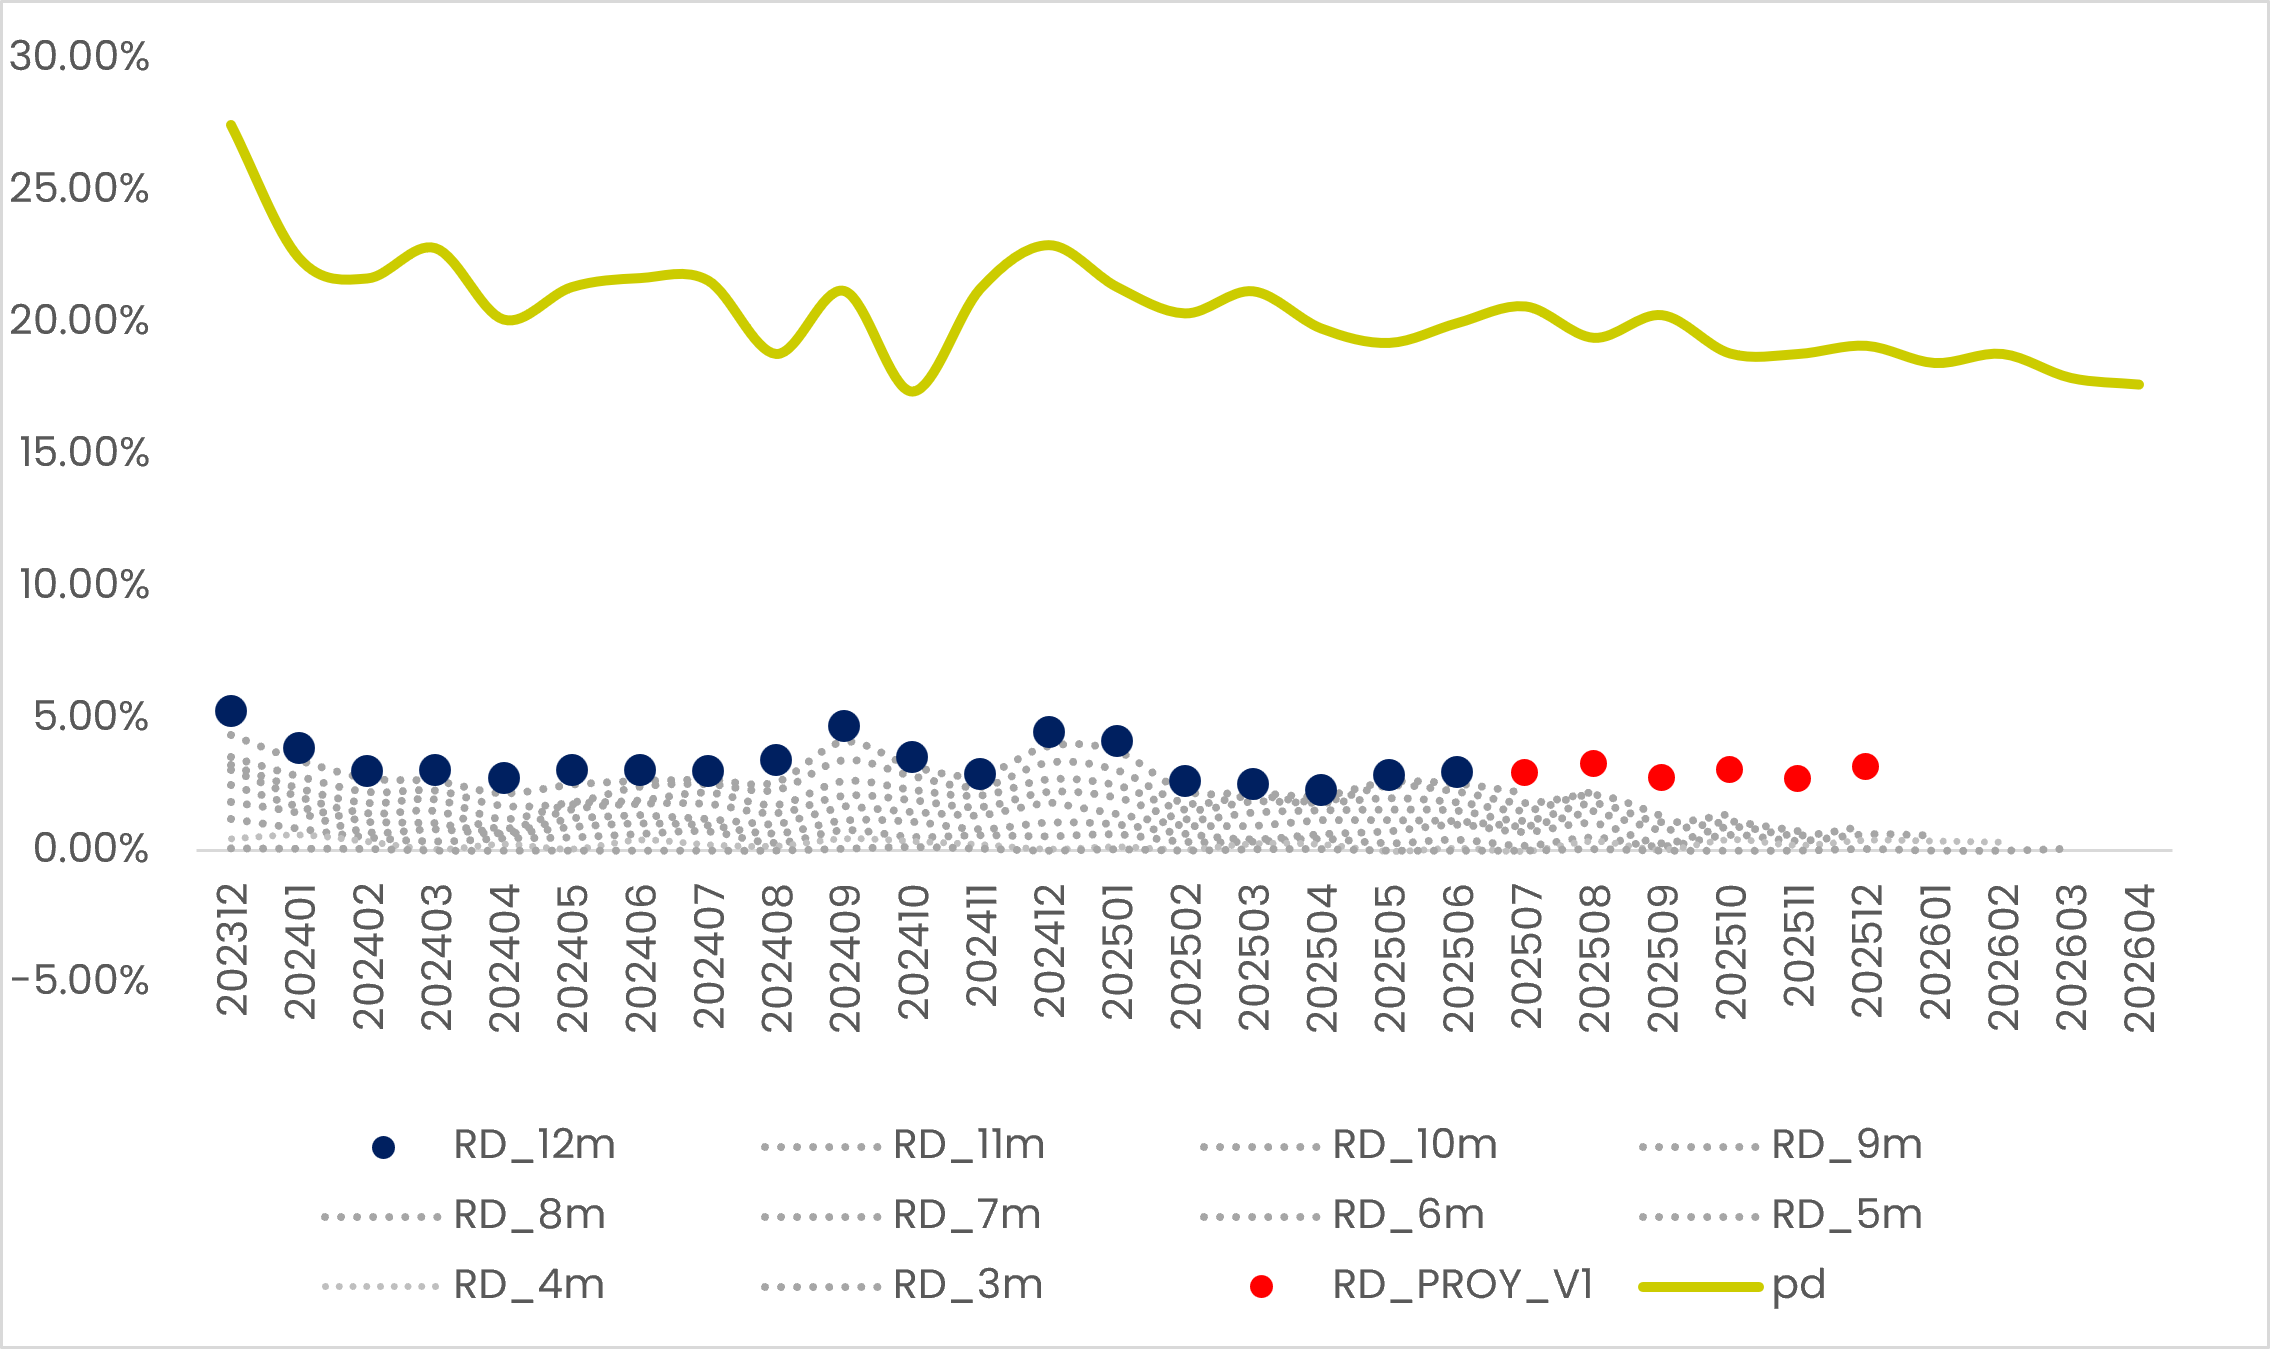
\includegraphics[width=0.88\textwidth]{figuras/global_pd_raw.png}\\[0.35cm]
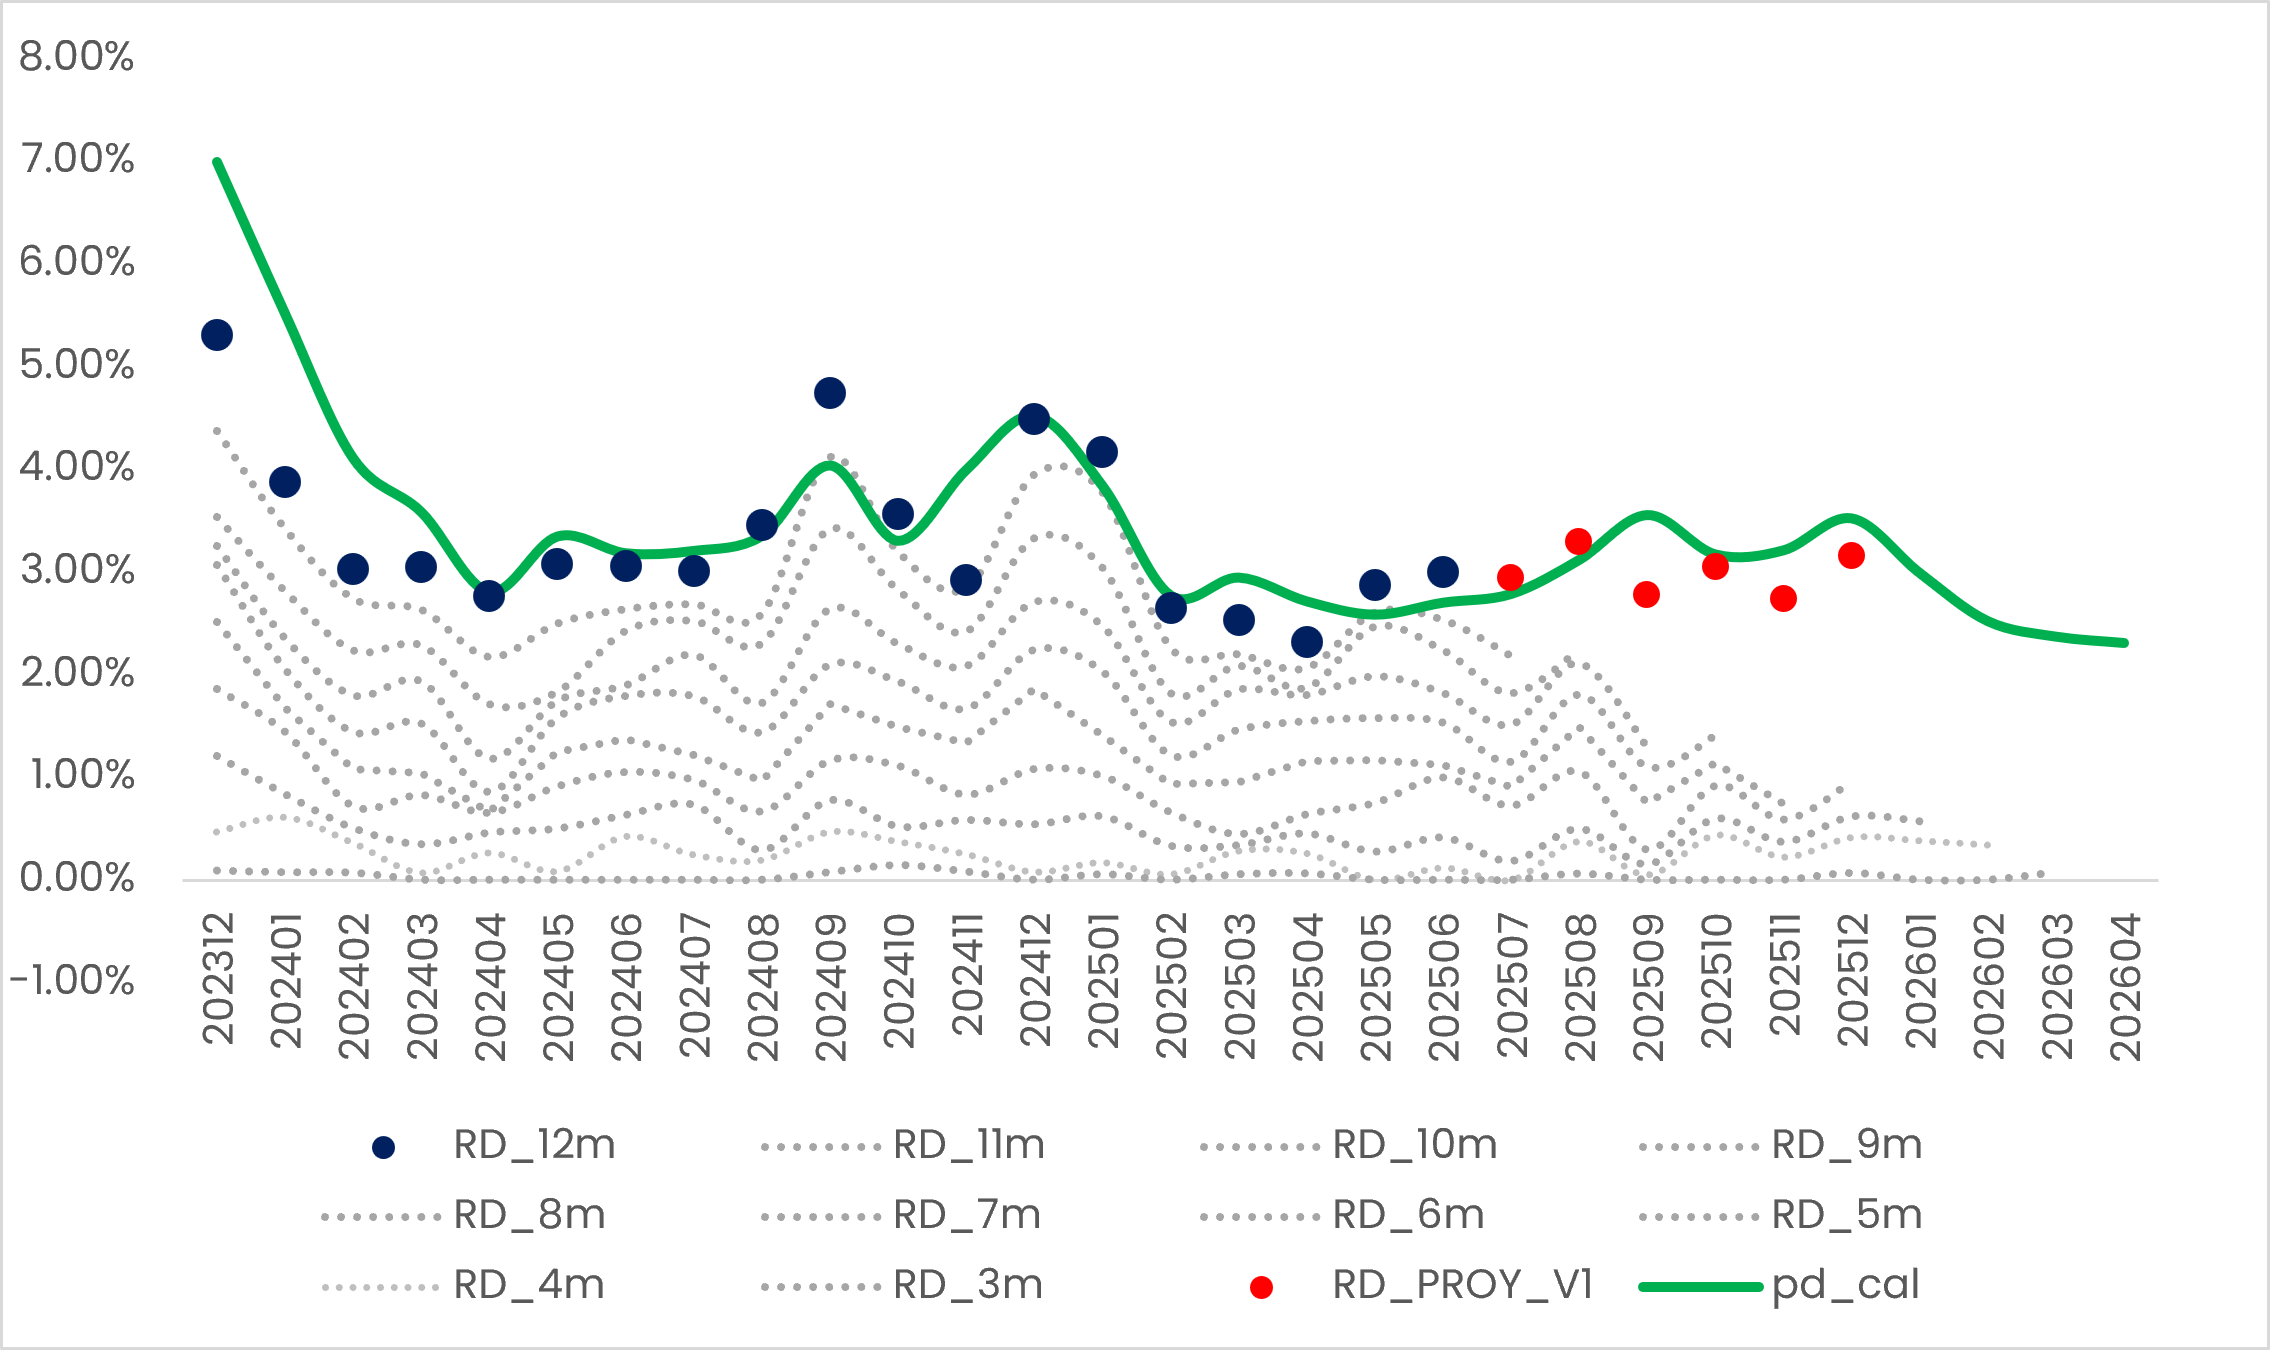
\includegraphics[width=0.88\textwidth]{figuras/global_pd_cal.png}
\caption{Global --- PD cruda (arriba) y PD calibrada PIT (abajo) contra la RD observada.
Obsérvese el cambio de escala del eje: la cruda vive en $[17\%,\,27\%]$ y la calibrada en
$[2{,}3\%,\,7{,}0\%]$. Umbrales y parámetros de calibración de referencia provisional, sujetos a
aprobación del Comité de Modelos.}\label{fig:rawcal_g}
\end{figure}

\begin{figure}[H]\centering
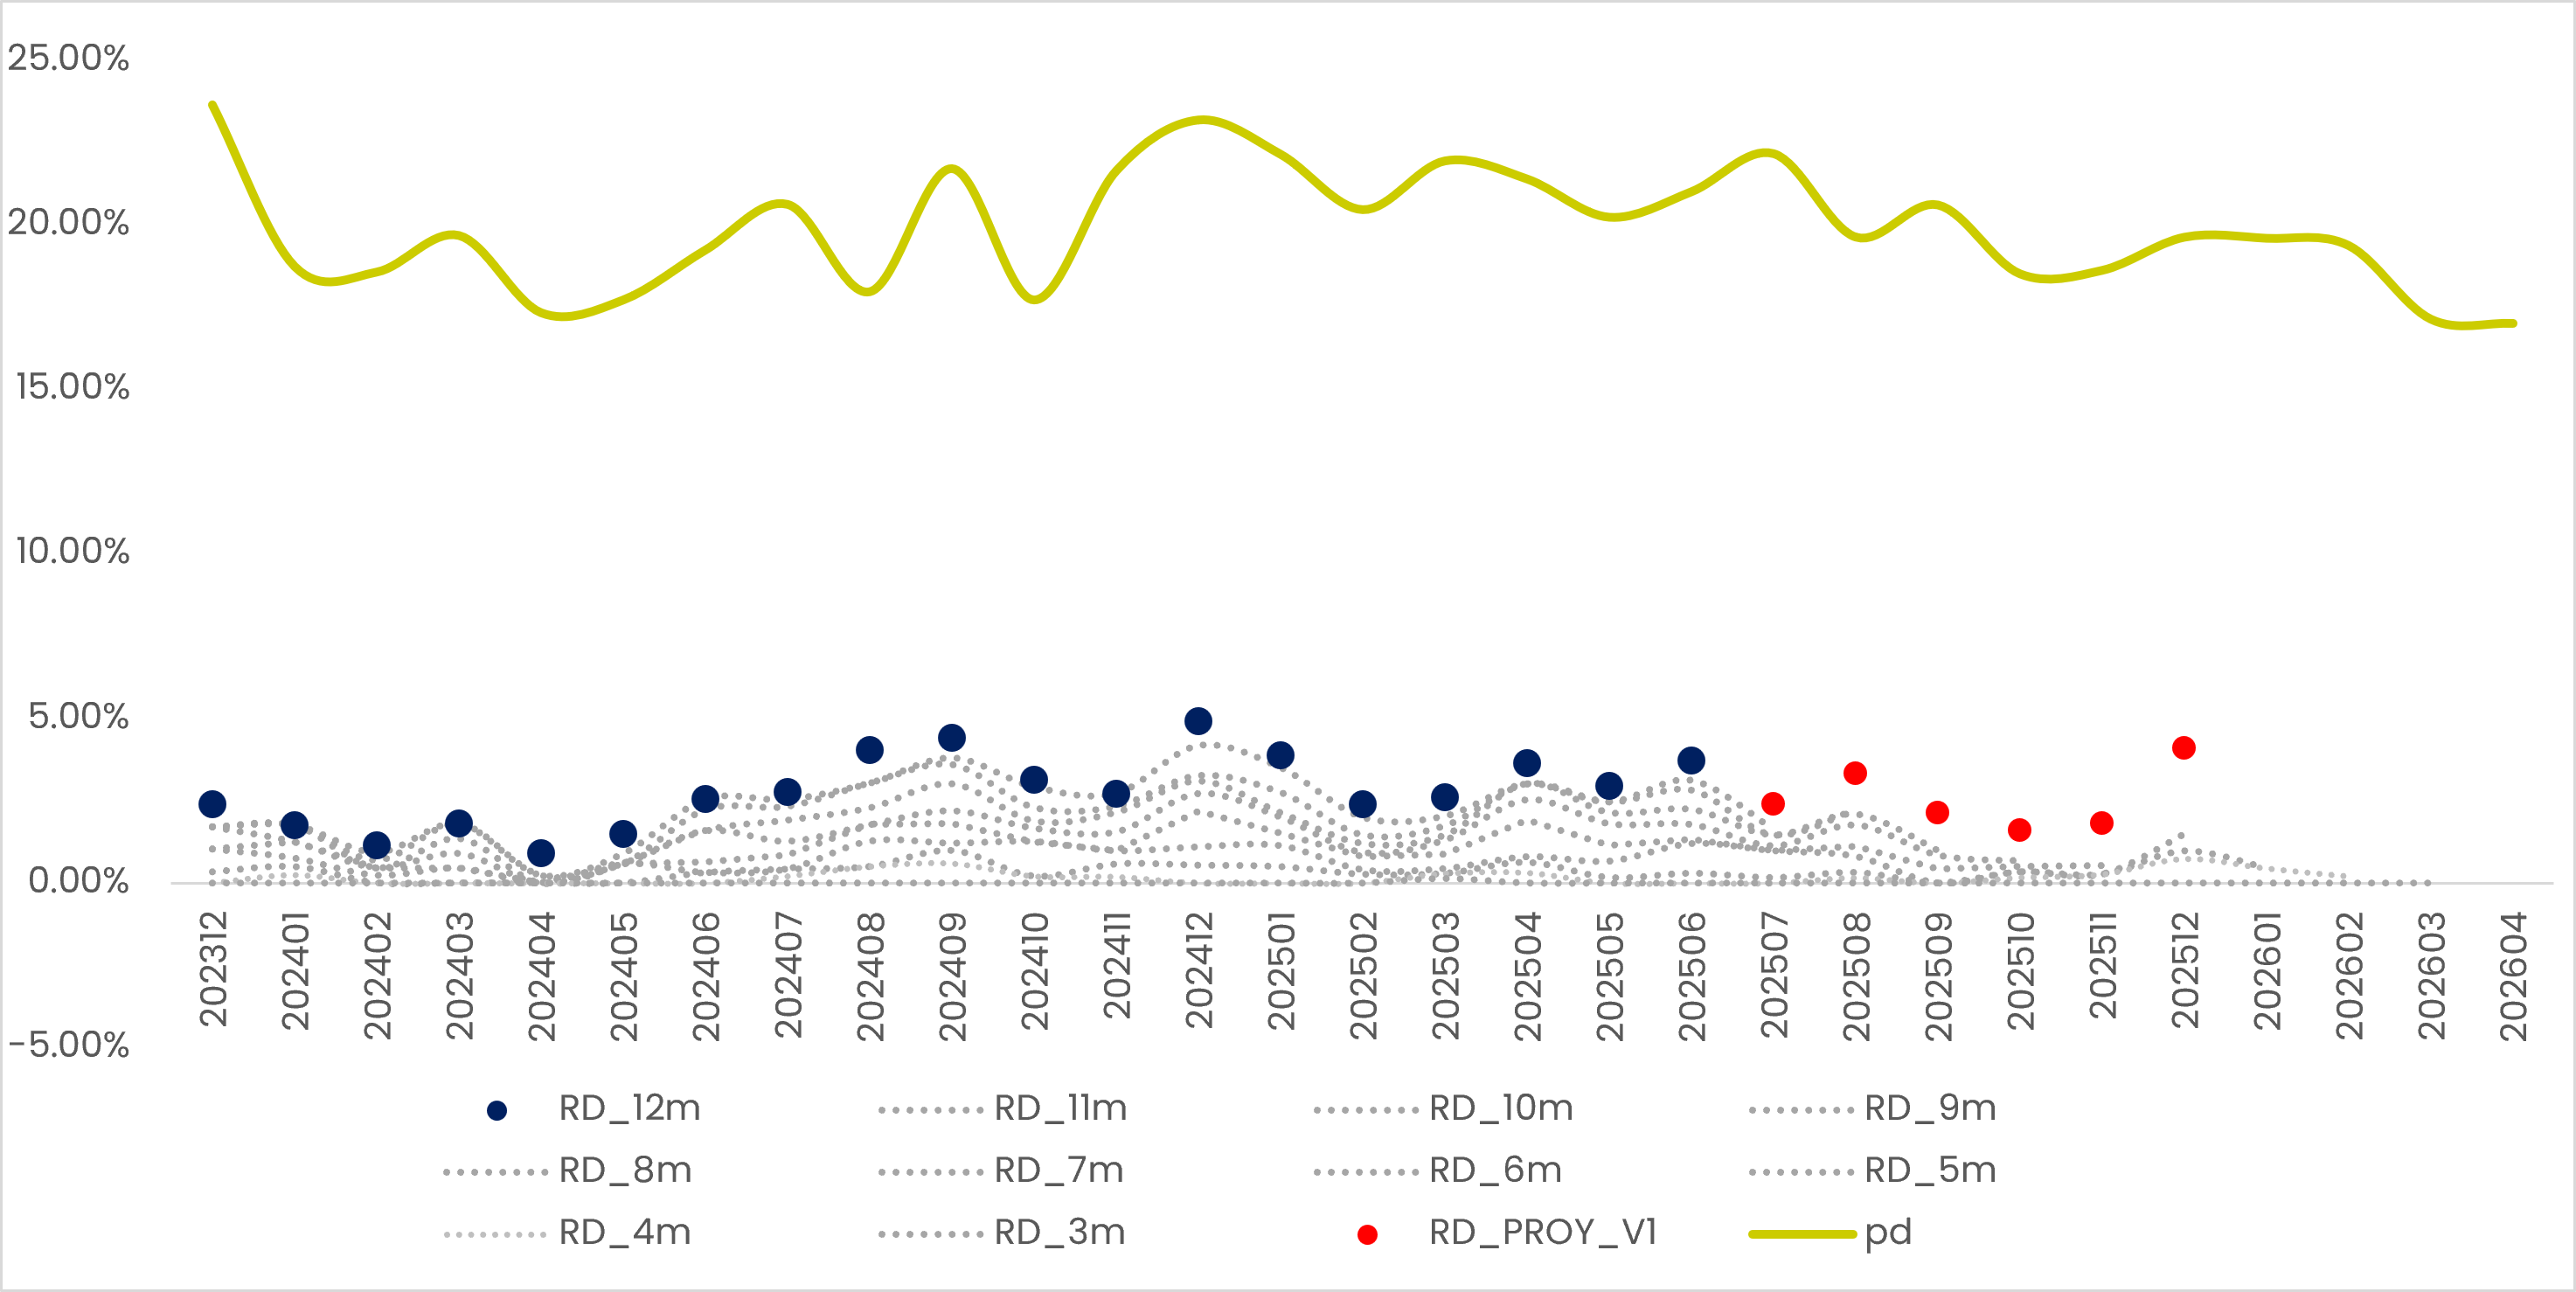
\includegraphics[width=0.88\textwidth]{figuras/dep_pd_raw.png}\\[0.35cm]
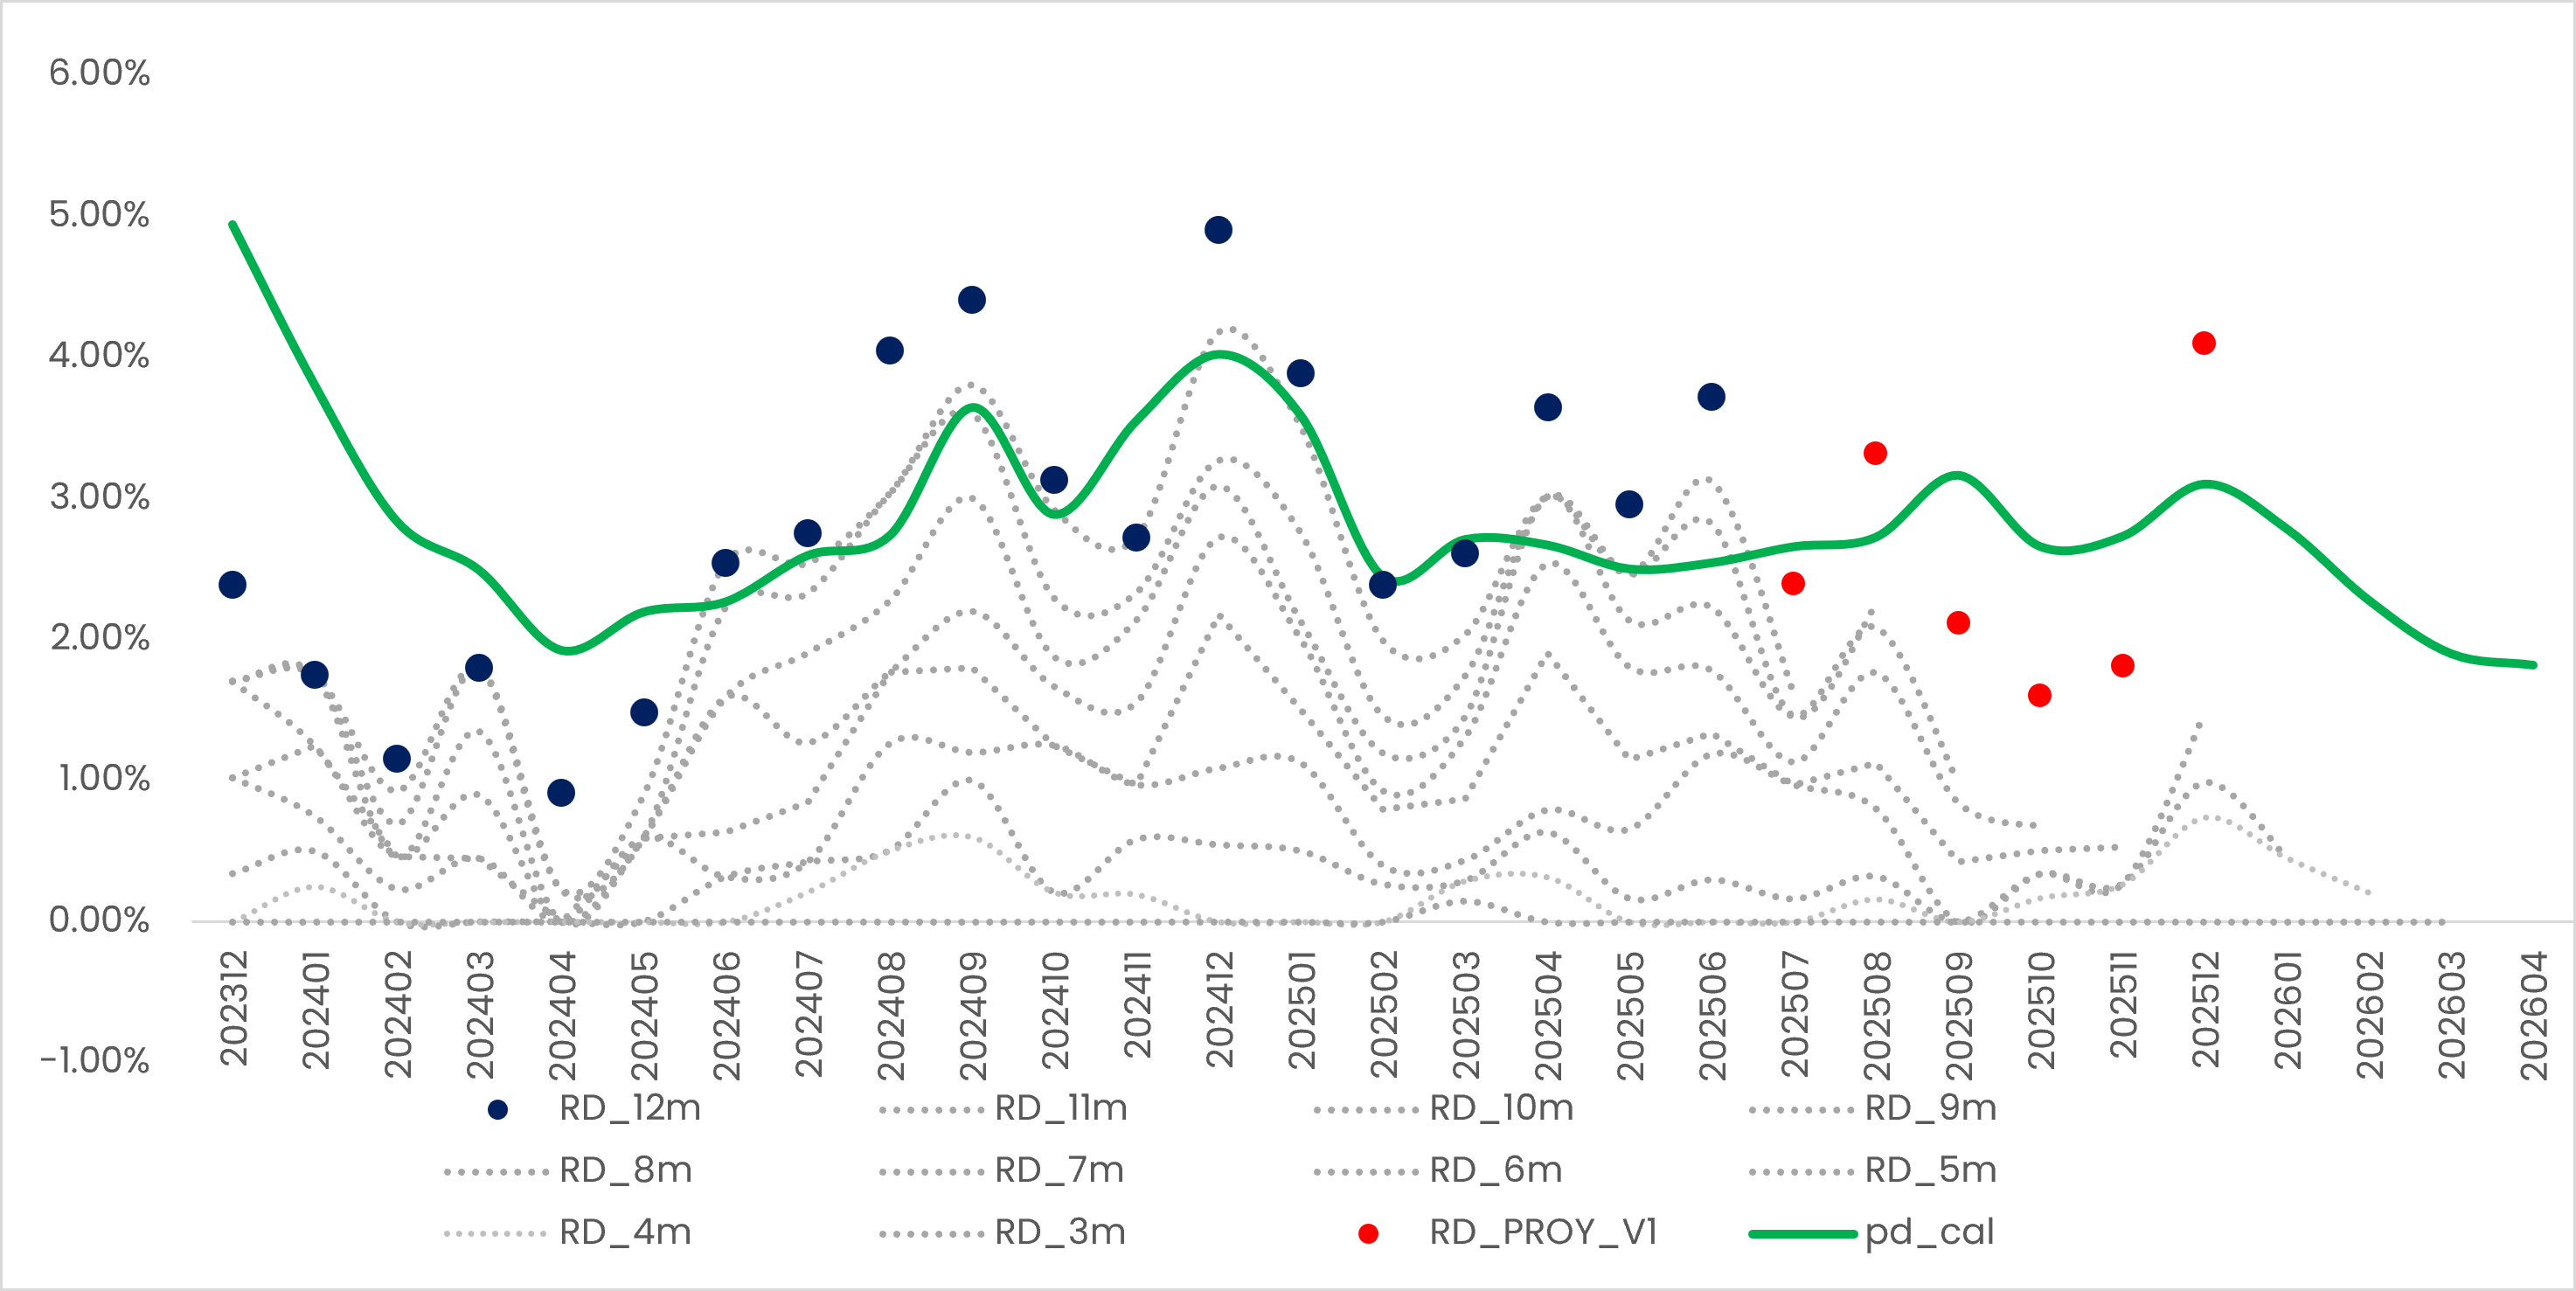
\includegraphics[width=0.88\textwidth]{figuras/dep_pd_cal.png}
\caption{Celda DEP --- PD cruda (arriba) y PD calibrada PIT (abajo) contra la RD observada.
PD cruda media $20{,}4528\%$ contra RD $2{,}9242\%$ ($6{,}99\times$); PD PIT media $2{,}9498\%$.
Umbrales y parámetros de calibración de referencia provisional, sujetos a aprobación del Comité de
Modelos.}\label{fig:rawcal_dep}
\end{figure}

\begin{figure}[H]\centering
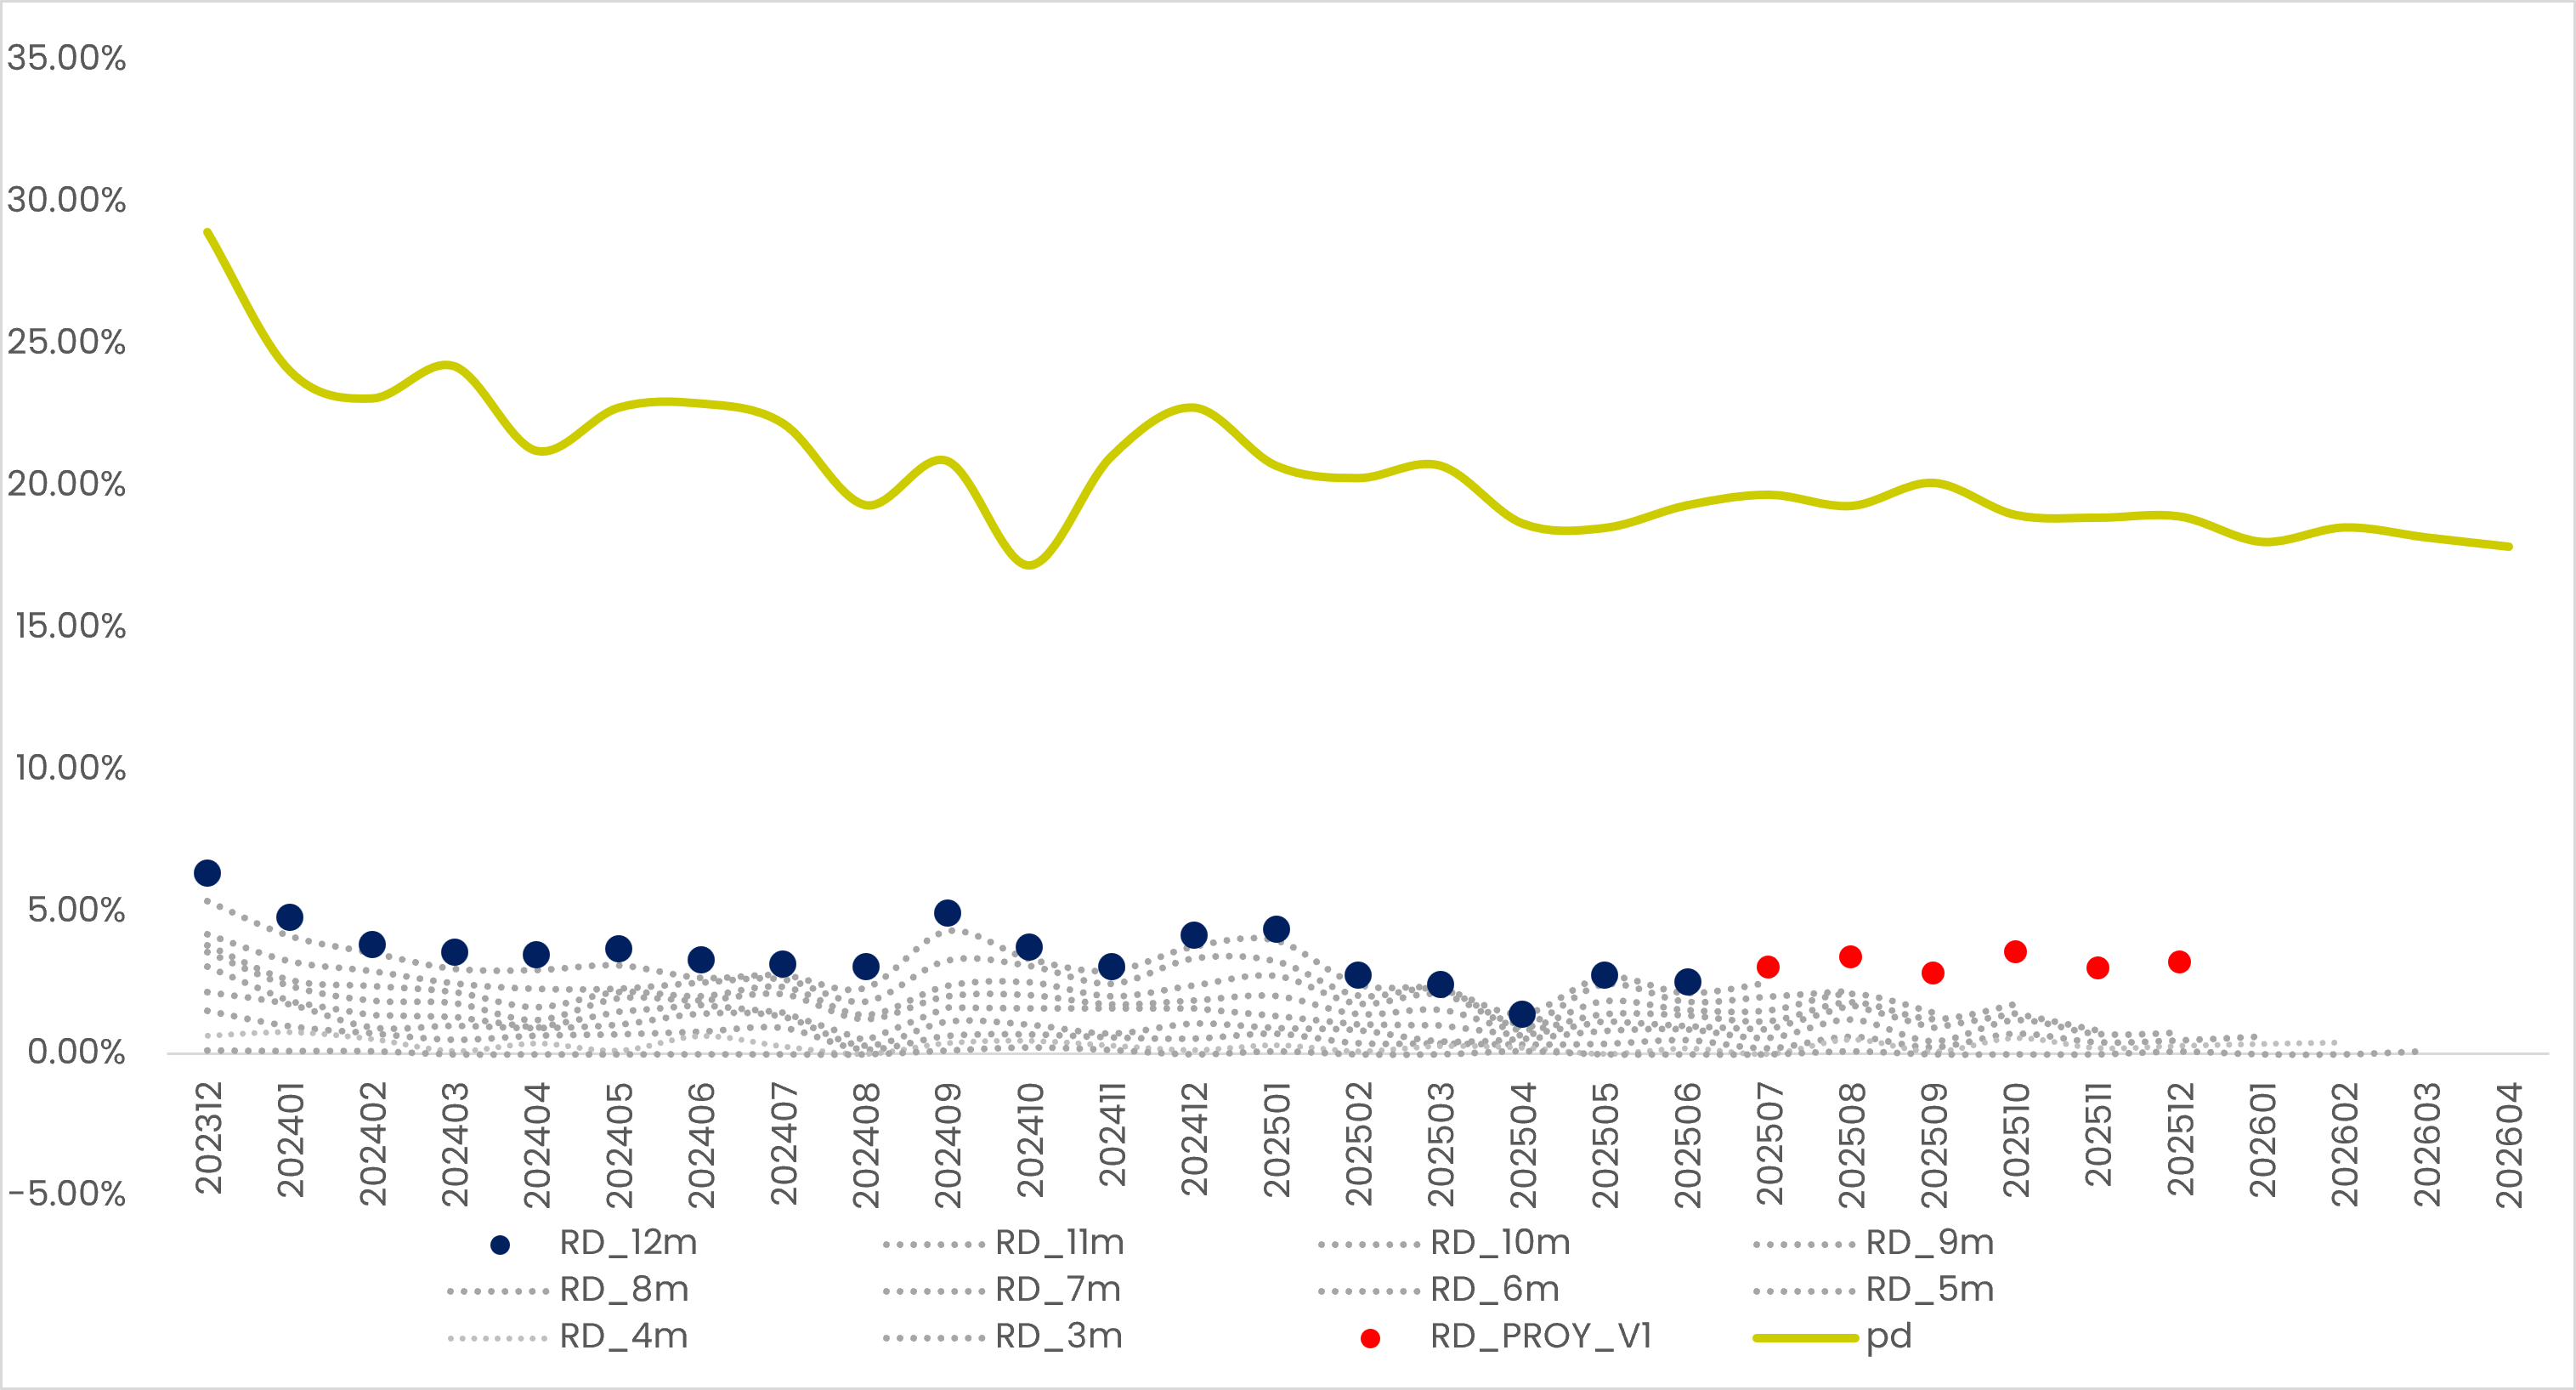
\includegraphics[width=0.88\textwidth]{figuras/nodep_pd_raw.png}\\[0.35cm]
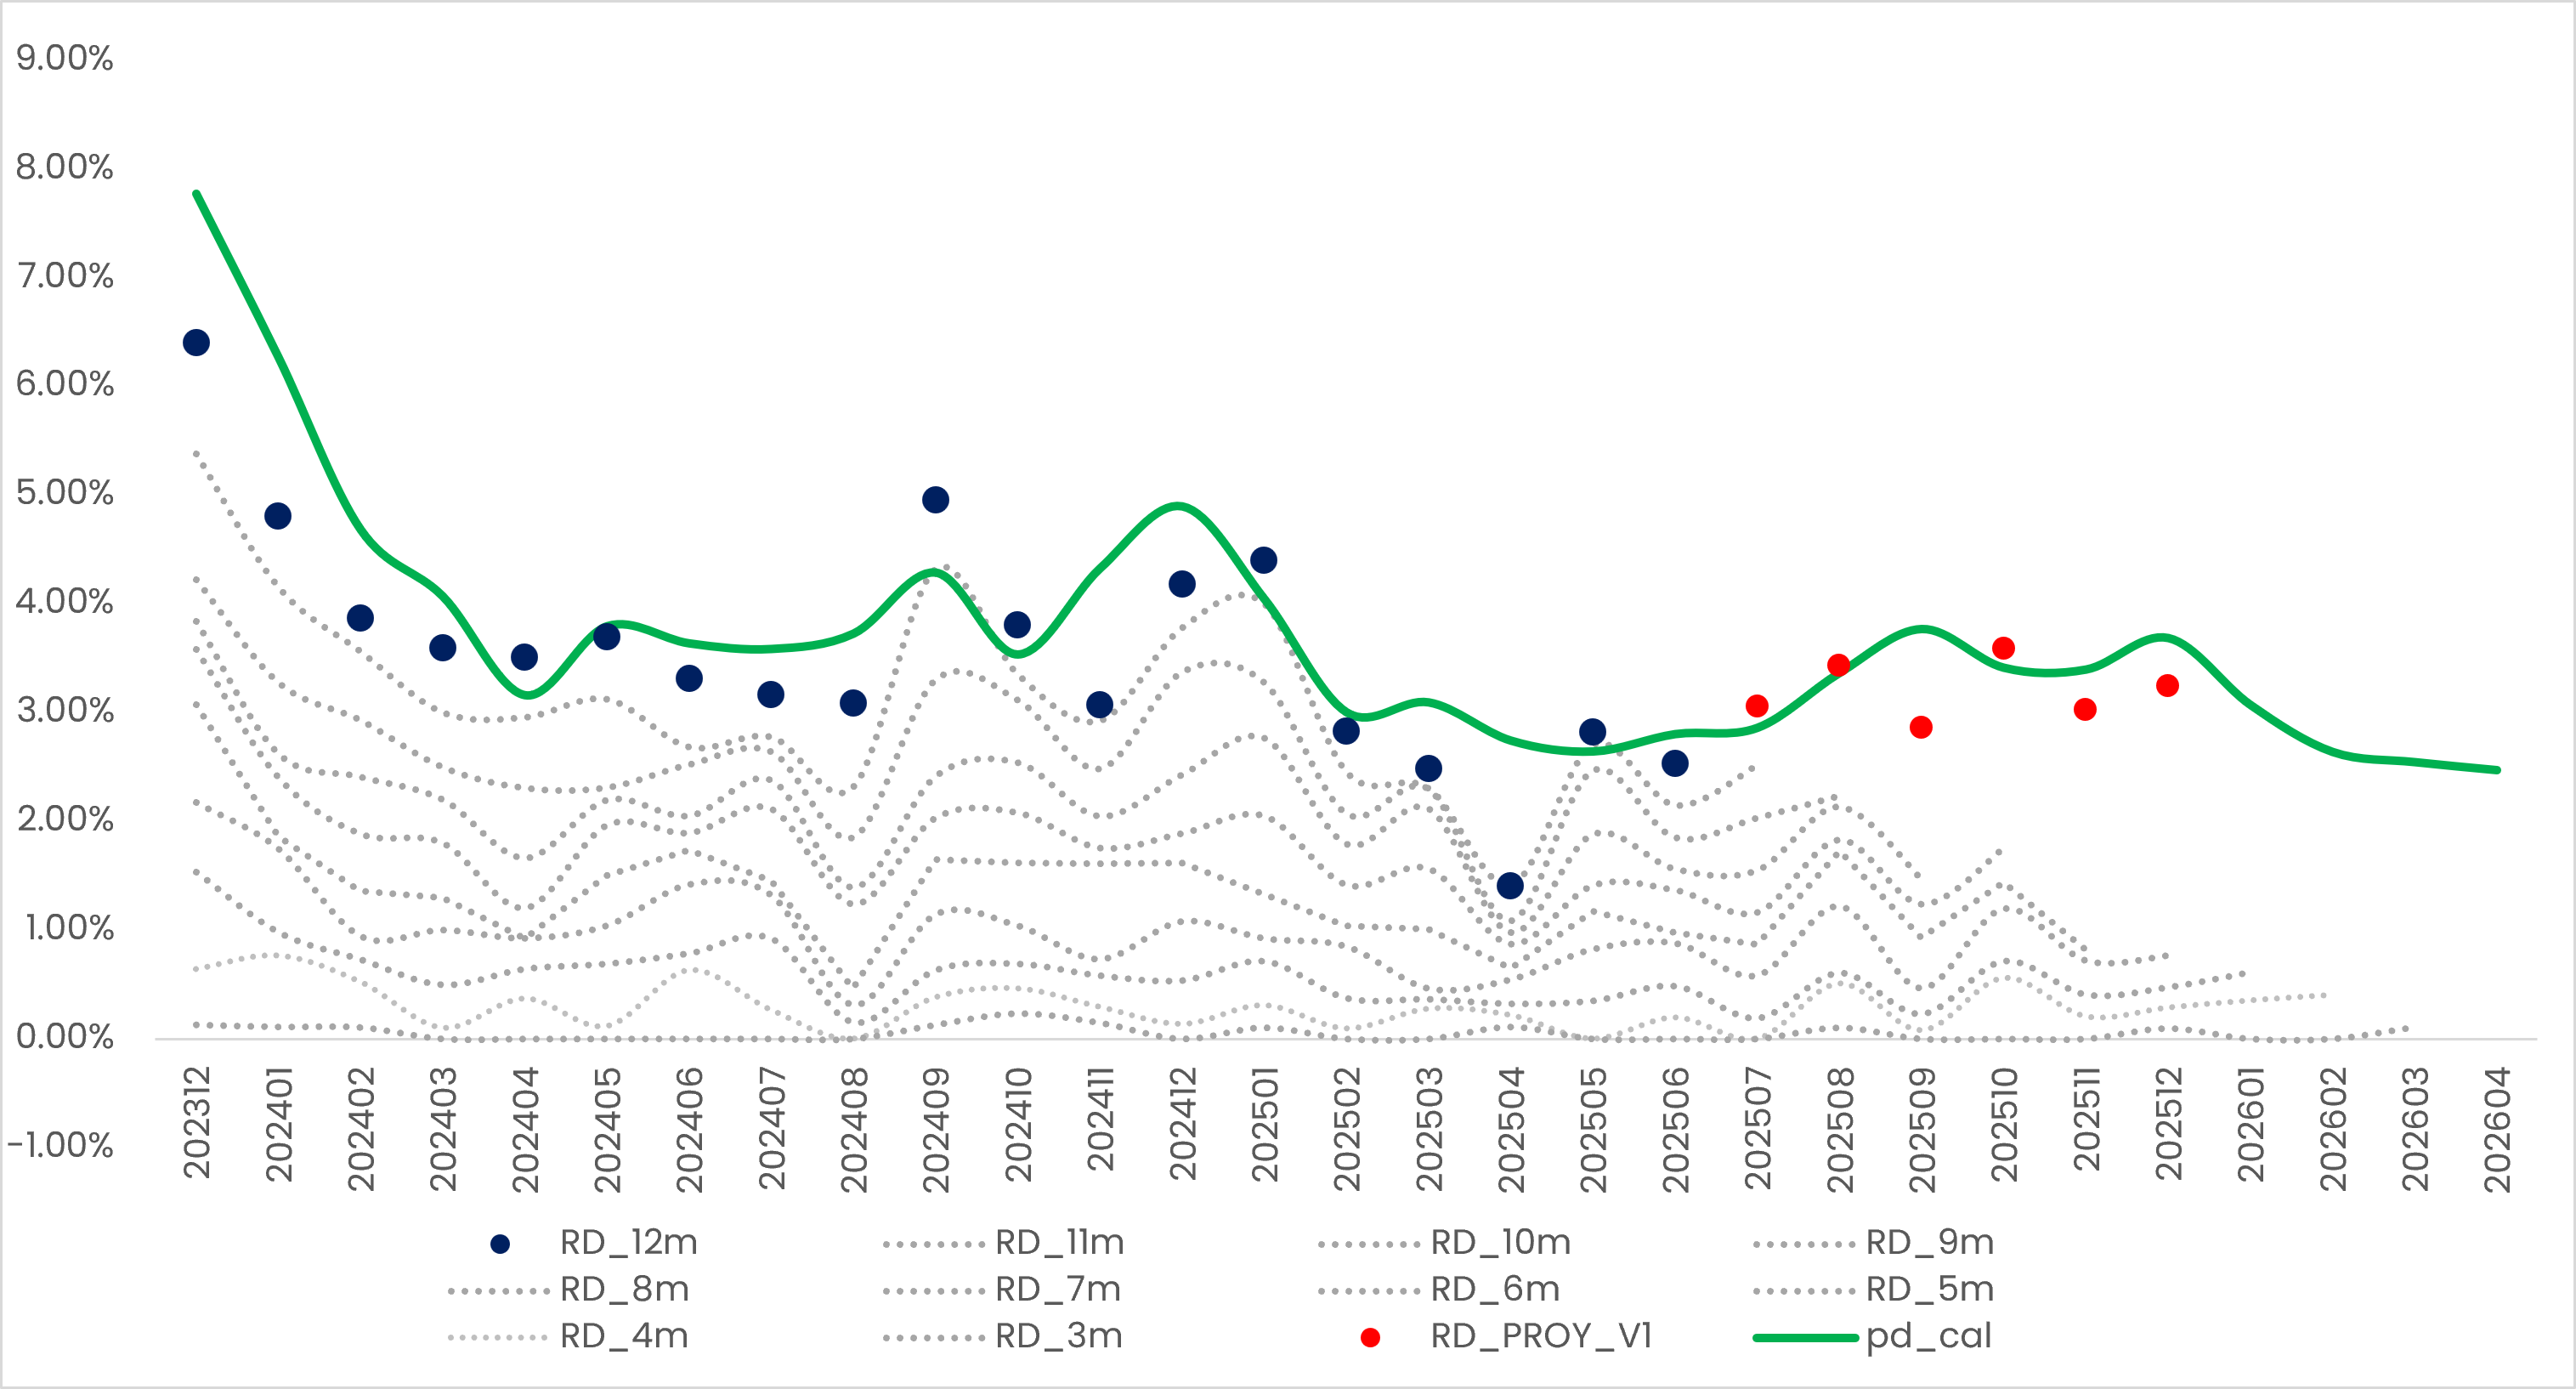
\includegraphics[width=0.88\textwidth]{figuras/nodep_pd_cal.png}
\caption{Celda NO DEP --- PD cruda (arriba) y PD calibrada PIT (abajo) contra la RD observada.
PD cruda media $21{,}4711\%$ contra RD $3{,}5405\%$ ($6{,}06\times$); PD PIT media $3{,}9440\%$.
Umbrales y parámetros de calibración de referencia provisional, sujetos a aprobación del Comité de
Modelos.}\label{fig:rawcal_nodep}
\end{figure}

\newpage
% ======================================================================

% ===== BLOQUE: F_sensib_REE.tex =====
\section{Sensibilidad y Limitaciones}
\label{sec:sens}

\subsection{Tratamiento de COVID y del episodio inflacionario, decidido con datos}
\label{sec:exclusiones}
El tratamiento de los dos regímenes atípicos se sometió a prueba formal, y el resultado es una
exclusión \textbf{asimétrica}, no uniforme, entre ellos:
\begin{itemize}[nosep]
  \item \textbf{COVID-2020 (202001--202012) $\to$ EXCLUIR de la LRA \emph{y} de $\rho$ (decisivo):}
    (a) el sustento es de dato, no de criterio ---la originación del producto cae de 1.383 cuentas
    en 202001 a \textbf{49} en 202004, y la RD12 de 202004 (12,24\%) descansa sobre esas 49
    observaciones---; (b) la exclusión es \textbf{determinante} para el modelo macro y no solo para el
    ancla, puesto que al retirarla \textbf{la cadena aborta}: el $R^2$ de la ventana \texttt{full}
    cae de 0,6110 a \textbf{0,3823}, por debajo del criterio de aceptación de régimen de 0,45;
    (c) sobre $\rho$, incluir COVID lo lleva de 0,038030 a \textbf{0,053543} ($+40{,}8\%$) y baja
    la $\PDPIT$ de Z1 en 8,8 bps.
    Encuadre: ECB par.~236(d)(iv) (período no representativo). $\Rightarrow$ exclusión sostenida.
  \item \textbf{Episodio inflacionario 2022--2023 (202207--202306) $\to$ EXCLUIR sólo de la LRA (no
    de $\rho$ ni del fit macro):} el criterio declarado es \textbf{IPC Lima anual $>6\%$ $=$
    2$\times$ el techo de la meta BCRP (3\%)}, verificable y citable, pero su ejecución presenta una
    inconsistencia que aquí se declara. El criterio se cumple en \textbf{202112--202306} (18 meses),
    mientras que la ventana efectivamente excluida es \textbf{202207--202306} (12 meses), obtenida
    con un rezago \emph{supuesto} de $\sim$12 meses entre el shock y el default. \textbf{Ese rezago no está medido y contradice al propio modelo macro}, que
    estima el rezago óptimo en \textbf{5 meses} (\texttt{lag5}, perfil unimodal); con el rezago del
    modelo la ventana sería 202205--202311. Sensibilidad de la exclusión completa: sin ella
    LRA $4{,}2263\%\to4{,}6881\%$ ($+46{,}2$ bps), $\PDPIT$ Z1 $+5{,}4$ bps, $\EC=-0{,}0875$, y
    además \emph{enciende} el driver \texttt{tipo\_ingreso\_cs}.
\end{itemize}

\begin{recuadro}{Exclusión asimétrica: COVID de LRA y $\rho$; spike sólo de LRA}
El tratamiento \textbf{no} es uniforme: COVID sale de las tres piezas (LRA, $\rho$ y fit macro),
mientras que el episodio inflacionario sale sólo del ancla. La asimetría importa por su dirección,
porque excluir dicho episodio \textbf{baja} la LRA en 46,2 bps; se trata, por lo tanto, de una
exclusión que \emph{reduce} la PD, de modo que su sustento debe ser explícito y no puede apoyarse
en un rezago no medido. Un dato cierra el círculo con \S\ref{sec:ft}: los meses del episodio
excluidos del ancla (12 meses, 202207--202306) y los meses que el cap fija en el piso (12 meses,
202203--202205 y 202209--202305) \textbf{se superponen en 9} (202209--202305). No es una identidad ---cada conjunto tiene 3 meses propios--- pero el solape
cubre el núcleo del episodio. El régimen que se excluye del ancla es el mismo que el cap trunca
en el factor; la calibración vigente, por lo tanto, \textbf{no ve el estrés de 2022--2023 ni por el
nivel ni por la amplitud}.
\end{recuadro}

\subsection{Sensibilidad OOT por Contracción de Ventana}
\label{sec:oot}
El backtest del semáforo es \textbf{100\% in-sample} (la ventana evaluada 202312--202506 \emph{es}
la ventana de fit, porque la frontera de madurez y el cierre de Z1 coinciden), de modo que la única
evidencia pseudo-OOT disponible se construye \textbf{contrayendo la ventana}: se re-corre toda la
cadena con \texttt{COHORTE\_FIN} adelantado $-1/-2/-3$ meses y se evalúa la $\PDPIT$ del modelo
recortado sobre los meses dropeados, que siguen maduros ($\Rightarrow$ backtest real, no
proyección). El Cuadro~\ref{tab:oot} reporta el barrido: los tres cortes quedan
\textbf{\textcolor{semverde}{$\blacksquare$}~VERDE} y los tres del lado de \textbf{sub-predicción
moderada} ($\EC_{oot}>0$), con la brecha \emph{decreciente} a medida que se recorta más.

\begin{table}[H]
\centering
\caption{Pseudo-OOT por contracción de ventana: modelo recortado evaluado sobre los meses
dropeados (RD12 ya cerrada)}
\label{tab:oot}
\small
\resizebox{\textwidth}{!}{%
\begin{tabular}{lcccc}
\toprule
\textbf{Ventana de fit} & \textbf{Meses dropeados} & \textbf{$\PDPIT$ Z1} & \textbf{$\EC_{oot}$} & \textbf{Semáforo} \\
\midrule
$\le$ 202506 (FINAL) & ---                 & 3,5775\%              & --- ($\EC$ in-sample $-0{,}0738$) & \textcolor{semverde}{$\blacksquare$} Verde \\
$\le$ 202505 ($-1$)  & 202506              & no publicado          & $+0{,}229$ & \textcolor{semverde}{$\blacksquare$} Verde \\
$\le$ 202504 ($-2$)  & 202505--202506      & no publicado          & $+0{,}218$ & \textcolor{semverde}{$\blacksquare$} Verde \\
$\le$ 202503 ($-3$)  & 202504--202506      & $+24{,}0$ bps         & $+0{,}107$ & \textcolor{semverde}{$\blacksquare$} Verde \\
\bottomrule
\end{tabular}%
}
\end{table}

\noindent\textbf{Sobre las configuraciones de cap.} La frontera sesgo--varianza de \emph{cinco
configuraciones de cap por driver} \textbf{no se evaluó en este expediente}: aquí el cap es \textbf{único y
global} (P5/P95 sobre la ventana de centrado, sin grilla por segmento) y la grilla de cinco
configuraciones no se corrió. Lo que sí está medido es el barrido de \texttt{F\_CAP\_QUANTILE}
sobre la cadena completa: $q=0{,}80$ cuesta $+10{,}4$ bps de $\PDPIT$ Z1 ($+10{,}7$ global),
$q=1{,}00$ (rango observado, sin capeo efectivo) cuesta $-1{,}2$ bps ($-2{,}2$ global), y las tres
configuraciones quedan \textcolor{semverde}{$\blacksquare$}~VERDE. Se declara como \textbf{no
medido} el sesgo OOT \emph{por configuración de cap}. La lectura relevante no es de nivel sino de
\textbf{asimetría}: el cap topa 18 de 92 meses ---12 en el piso y 6 en el techo---, de los cuales \textbf{15 caen dentro de la ventana de estimación} (12 en piso, 3 en techo), y su consecuencia
cambia de signo según el régimen ---en régimen benigno topa el techo y es conservador, en estrés
topa el piso y es anti-conservador--- (ver Limitaciones, \S\ref{sec:limitaciones}).

\subsection{Sensibilidad por LOO temporal (66 particiones)}
\label{sec:loo}
Como prueba de estabilidad adicional se realiza un \emph{leave-one-out} temporal sobre el modelo
macro. El procedimiento \textbf{re-estima el probit} dejando fuera cada uno de los \textbf{66 meses}
de la ventana de fit (201901--202506, excluido COVID) ---las 66 particiones o \emph{folds}--- y
registra el movimiento de los coeficientes y del criterio de aceptación de régimen. El ejercicio
evalúa dos aspectos: cuánto se desplazan los coeficientes y cómo se comporta la cadena cuando se le
retira evidencia reciente.

\textbf{(1) Estabilidad de coeficientes.} La estructura se mantiene en las 66 particiones: ningún
mes individual resulta influyente, la pendiente macro se desplaza menos del $1{,}2\%$ de su valor y
el signo \emph{nunca} cambia. El criterio de aceptación de régimen se satisface en las 66
particiones, y su ventana determinante (\texttt{reciente}, 18 meses) nunca cae por debajo de
0,5288, de manera que conserva \textbf{7,9 puntos de $R^2$} de holgura sobre el umbral de 0,45.

\begin{table}[H]
\centering
\caption{Estabilidad del modelo macro por LOO temporal: FINAL (66 meses) vs las 66 particiones}
\label{tab:loo_coef}
\small
\resizebox{\textwidth}{!}{%
\begin{tabular}{l cc cc}
\toprule
 & \multicolumn{2}{c}{\textsc{Coeficientes}} & \multicolumn{2}{c}{\textsc{Gate de régimen}} \\
\cmidrule(lr){2-3}\cmidrule(lr){4-5}
\textbf{Parámetro} & \textbf{FINAL} & \textbf{LOO (66 folds)} & \textbf{FINAL} & \textbf{LOO (66 folds)} \\
\midrule
Variable macro / lag & \multicolumn{4}{c}{idéntica en los 66 folds (\texttt{IPC\_Lima\_var\_12m\_lag5\_ma6}, lag 5)} \\
$b_0$              & $-1{,}900196$ & media $-1{,}900203$ $\cdot$ sd 0,003173 $\cdot$ \textbf{CV 0,17\%} & --- & --- \\
$b_1$              & $+0{,}658342$ & media $+0{,}658391$ $\cdot$ sd 0,007740 $\cdot$ \textbf{CV 1,18\%} & --- & --- \\
Rango de $b_0$     & ---           & {\footnotesize $[-1{,}9084,\,-1{,}8901]$} & --- & --- \\
Rango de $b_1$     & ---           & {\footnotesize $[+0{,}6398,\,+0{,}6833]$} & --- & --- \\
$R^2$ ventana \texttt{full}     & 0,6110 & --- & \multicolumn{2}{c}{pasa} \\
$R^2$ ventana \texttt{reciente} (determinante) & 0,5564 & --- & \multicolumn{2}{c}{mín.\ \textbf{0,5288} $\cdot$ máx.\ 0,6171} \\
Gate $R^2\ge0{,}45$ en las 4 ventanas & pasa & --- & \multicolumn{2}{c}{\textbf{PASS en 66 de 66 folds}} \\
\bottomrule
\end{tabular}}%
\end{table}

\textbf{(2) Predicción sobre meses no vistos (RD12 cerrada).} El LOO mes a mes no genera meses
fuera de muestra ---al quitar un mes del fit, ese mes sigue teniendo RD12 cerrada pero la cadena se
reconstruye sobre casi la misma información---, de modo que la prueba \emph{predictiva} la aporta
la contracción de ventana de \S\ref{sec:oot}. El Cuadro~\ref{tab:loo_pred} contrasta el modelo
recortado a $\le202503$ contra el FINAL sobre el agregado de 202504--202506. El modelo recortado
predice cerca del FINAL, con una brecha de aproximadamente $+24$ bps en $\PDPIT$ Z1, y queda del
lado \textbf{estricto} ---sub-predicción, $\EC_{oot}=+0{,}107$--- y no del conservador. Es el mismo
signo que arrojan los tres cortes del barrido.

\begin{table}[H]
\centering
\caption{Contracción a $\le202503$: predicción sobre 202504--202506 (pool, RD12 cerrada)}
\label{tab:loo_pred}
\small
\resizebox{\textwidth}{!}{%
\begin{tabular}{lccccc}
\toprule
\textbf{Agregado} & \textbf{$\PDPIT$ FINAL} & \textbf{$\PDPIT$ recortado} & \textbf{$\EC$ in-sample} & \textbf{$\EC_{oot}$} & \textbf{$gap$ rec.$-$FIN} \\
\midrule
GLOBAL (Z1)   & 3,5775\% & 3,8175\% & $-0{,}0738$ & $+0{,}107$ & $+24{,}0$ bps \\
DEP           & 2,9498\% & no publicado & $-0{,}0087$ & no medido & no medido \\
NO DEP        & 3,9440\% & no publicado & $-0{,}1023$ & no medido & no medido \\
\bottomrule
\end{tabular}%
}
\end{table}
\noindent El desglose \textbf{por segmento} del ejercicio de contracción \textbf{no se midió}: el
barrido publica el agregado y no reestima el $\EC_{oot}$ por celda, y se declara como tal en vez de
imputarse. El ejercicio no altera el modelo FINAL, que se mantiene congelado en $\le202506$. Una
advertencia sobre el alcance de esta evidencia: con $\rho_1=0{,}816$ en la serie de RD, quitar un
mes elimina muy poca información independiente, de modo que el LOO prueba \textbf{estabilidad de
estimación}, no \textbf{capacidad predictiva} ni ---sobre todo--- la \emph{selección} de la variable
macro (limitación 1 de \S\ref{sec:limitaciones}).

\subsection{Sensibilidad a LRA, $\rho$ y $\lambda$}
Los tres parámetros se barren por separado. Cada cuadro recoge las alternativas evaluadas, el
valor que produce cada una y su efecto sobre la \PDPIT{} de Z1, de modo que la magnitud de cada
decisión sea directamente comparable.

\paragraph{Ancla de largo plazo (\LRA).} El valor vigente es la mediana sobre los 54 meses de la
ventana, $4{,}2263\%$, que es \textbf{el mínimo de las cuatro variantes} evaluadas.

\begin{table}[H]
\centering
\caption{\LRA: variantes del estimador y de la ventana}
\label{tab:sens_lra}
\small
\begin{tabular}{lrrr}
\toprule
\textbf{Variante} & \textbf{\LRA} & \textbf{$\Delta$ vs vigente} & \textbf{$SE$ \emph{bootstrap}} \\
\midrule
\textbf{Mediana, 54 meses (vigente)} & \textbf{4,2263\%} & --- & 59,72 bps \\
Media, misma ventana                 & 4,3950\% & $+16{,}9$ bps & 37,92 bps \\
Mediana, ventana completa            & 4,5259\% & $+29{,}9$ bps & --- \\
Mediana, excluyendo sólo COVID       & 4,6881\% & $+46{,}2$ bps & --- \\
\bottomrule
\end{tabular}
\end{table}

\noindent La elección vigente desplaza la $\PDPIT$ de Z1 en $-15{,}0$ bps. La diferencia entre mediana y media no es significativa ($P(\text{mediana}_{boot}>\text{media obs.})=0{,}436$). Por segmento, la \LRA{} de DEP descansa sobre 30 meses ($SE=49{,}93$ bps) frente a los 54 de NO DEP ($SE=60{,}05$ bps).

\noindent Las dos premisas escritas en la configuración están \textbf{medidas y resultan falsas}
sobre esta serie: la mediana no es la desviación \emph{conservadora} ---queda $16{,}9$ bps por
debajo de la media de su misma ventana--- ni la \emph{robusta} ---su error estándar es
$1{,}57\times$ el de la media---. La elección se documenta por tanto como \emph{elección de
estimador} y se declara como incertidumbre: no se cambia el valor, se cambia la razón.

\paragraph{Correlación de activos ($\rho$).} El valor vigente es $0{,}038030$, estimado por método
de momentos sobre 66 meses ($\mathrm{var}(\Norm^{-1}(\RD))=0{,}039534$). Es poco influyente en el
rango relevante.

\begin{table}[H]
\centering
\caption{$\rho$: configuraciones evaluadas y efecto del piso}
\label{tab:sens_rho}
\small
\resizebox{\textwidth}{!}{%
\begin{tabular}{lrll}
\toprule
\textbf{Configuración} & \textbf{Valor} & \textbf{Efecto en $\PDPIT$ Z1} & \textbf{Estado} \\
\midrule
\textbf{Momentos, 66 meses (vigente)} & \textbf{0,038030} & --- & En uso \\
Piso declarado                        & 0,0332 & Ninguno & \textbf{No activo}; holgura 12,7\% \\
Piso reducido a la mitad              & 0,0166 & Ninguno & No activo \\
Piso elevado                          & 0,0498 & $-6{,}7$ bps & Se activa \\
Fórmula IRB evaluada en la \LRA       & 0,0596 & --- & Publicado y \textbf{no usado} \\
\bottomrule
\end{tabular}%
}
\end{table}

\noindent La cita normativa del piso \textbf{no reproduce su número}: la fórmula IRB \emph{other
retail} evaluada en la \LRA{} de este portafolio da $0{,}0596$, mientras que $0{,}0332$ corresponde
a $\rho_{Basel}$ evaluado en $\PD=10{,}58\%$, que no es la \PD{} de esta cartera. Hoy la
discrepancia es inocua porque el piso no está activo.

\paragraph{Carga cíclica ($\lambda$).} El valor vigente es $\lambda=1$, que es el extremo superior
del rango ejecutable: el código de producción impone la restricción $0<\lambda\le1$, de modo que
todo $\lambda>1$ detiene la cadena.

\begin{table}[H]
\centering
\caption{$\lambda$: barrido con la restricción relajada, y estimadores no ejecutables}
\label{tab:sens_lambda}
\small
\begin{tabular}{rlp{7.2cm}c}
\toprule
\textbf{$\lambda$} & \textbf{$\PDPIT$ Z1} & \textbf{Origen del valor} & \textbf{Ejecutable} \\
\midrule
0,10  & 3,9387\% & Amortiguación extrema & Sí \\
0,50  & 3,7645\% & Amortiguación; cuesta $+0{,}57$ a $+0{,}98\%$ de \emph{logloss} & Sí \\
0,75  & 3,6669\% & Extremo inferior del rango defendible & Sí \\
\textbf{1,00} & \textbf{3,5775\%} & \textbf{Vigente}: carga plena, sin amortiguación & \textbf{Sí} \\
1,25  & 3,4961\% & Óptimo de MSE fuera de muestra (embargo 12 meses) & \textcolor{semrojo}{No} \\
1,344 & 3,4675\% & MLE binomial, IC95\% $[1{,}2611,\,1{,}4272]$ & \textcolor{semrojo}{No} \\
2,00  & 3,2976\% & Referencia del barrido & \textcolor{semrojo}{No} \\
\bottomrule
\end{tabular}
\end{table}

\noindent Los siete trimestres del semáforo permanecen verdes hasta $\lambda=1{,}25$.

\noindent Tres mediciones independientes convergen en que $\lambda=1$ es el valor correcto, y no
sólo el permitido. \textbf{Primera:} $\lambda$ entra siempre multiplicando a $\sqrt{\rho}$, de modo
que adoptar $1{,}344$ equivale a declarar $\rho_{ef}=\rho\lambda^2=0{,}068710$ ---un 81\% por
encima de la $\rho$ medida y por encima incluso de la referencia IRB de $0{,}0596$---, es decir una
re-estimación implícita y no declarada de $\rho$. \textbf{Segunda:} al re-estimar el mismo MLE con
$\ft$ sin capar, el máximo cae a $1{,}0926$; el $\lambda$ alto mide entonces la compresión del cap
y no una respuesta cíclica mayor. \textbf{Tercera:} con $\ft$ sin capar y $\lambda=1$, la
verosimilitud en $\rho$ da $0{,}037565$ frente a $0{,}038030$ por momentos ---un $1{,}2\%$ de
diferencia---, de manera que el modelo cierra consigo mismo en $\lambda=1$. La amortiguación queda
además refutada por el barrido. Todo el análisis de $\lambda$ es condicional al factor macro
vigente.

\subsection{Registro de Decisiones Metodologicas}
\begin{table}[H]
\centering
\caption{Registro de decisiones (resumen)}
\scriptsize
\setlength{\tabcolsep}{4pt}
\begin{tabular}{lp{4.3cm}p{7.3cm}}
\toprule
\textbf{ID} & \textbf{Decisión} & \textbf{Sustento} \\
\midrule
A10 & Frontera de madurez \texttt{COHORTE\_FIN}$=$202506 & mecánica del calendario (\texttt{codmes\_mrm}$+12>202606$); corte limpio verificado (100\% sin m12 desde 202507), no degradación gradual \\
A36 & \texttt{flg\_scope\_ree} y \texttt{flg\_clean} como ejes separados & el fit es \texttt{scope}$=1$ AND \texttt{clean}$=1$ AND \texttt{calib}$=1$; población 119.018 de 119.254 (bucket~99 $=178$, dirty $=58$) \\
A49 & \texttt{rd12\_ventana\_completa} no se usa para elegir la macro & es serie de sobrevivientes: RD del fit 3,31\% $\to$ 1,48\% \\
A51 & Variable macro seleccionada por embudo con signo impuesto \emph{a priori} & meseta de $R^2$ 0,6110 vs 0,6007; perfil por rezago unimodal con pico en \texttt{lag5} \\
A55 & No cambiar la segmentación (BetaCal por \texttt{tipo\_ingreso\_dep}) & registrada como «no hay evidencia para cambiar», \textbf{no} como «la vigente es superior»; diseño subpotenciado factor 2--3 \\
A56 & BetaCal con restricción de Kull ($a\ge0$, $b\ge0$) por KKT real & único cambio de modelo que la evidencia soporta; efecto hoy $=0$, beneficio preventivo (sin ella, 8 de 10 refits dan $b<0$ en DEP) \\
A57 & \texttt{LEVEL\_CHECK\_THRESHOLD} de 50 bps a \textbf{0} (anclar siempre) & 50 bps dominado en ambos criterios; costo OOT de anclar siempre $+0{,}088\%$ de logloss, $p=0{,}803$ \\
A59 & $\lambda$ se mantiene en 1,0 & correcta en su conclusión; \textbf{incompleta en su fundamento} original (no había alternativa corrible) --- completada arriba \\
A62 & Ventana de centrado de $\ft$ fijada a la de la LRA (54~m) & Dömötör e Illés (2025) eq.~(9); antes se centraba sobre 76 meses, 10 de ellos sin RD observada. Es la sensibilidad más grande de la cadena ($-32{,}5$ bps y el $\EC$ cambia de signo) \\

A66 & Horizonte de proyección topado en 6 meses adelante & instrucción del usuario; corta 202601, que descansaba en 6 defaults con factor 11,667 \\
A68 & \texttt{PROY\_VENTANA\_INICIO} de 201901 a 202401 & 202401 es el arranque del régimen que \texttt{REGIME\_WINDOWS['reciente']} ya declaraba por decisión anterior e independiente; el backtest confirma ($-1{,}6$ vs $+90{,}7$ bps de sesgo), no elige \\
A69 & Los Excel publican las \textbf{cinco} variantes de proyección & \texttt{RD\_PROY} / V1 / V2 / \texttt{V3\_MOM} / V3, publicadas en paralelo para contraste lado a lado \\
\bottomrule
\end{tabular}
\end{table}
\noindent\textbf{Decisiones abiertas al cierre de este corte:} A50, A52 (revisión de $\lambda$, cerrada
metodológicamente arriba pero pendiente de la decisión sobre la guarda de código), A58
(multiplicador de banda $\EC$ $\times1$ vs $\times2$), A61 (reemplazo del Excel vigente) y A67 (los
dos topes de horizonte de proyección).

\subsection{Limitaciones}
\label{sec:limitaciones}
\noindent El Cuadro~\ref{tab:limitaciones} resume las limitaciones con su magnitud medida y su
estado; el desarrollo de cada una sigue a continuación.

\begin{table}[H]
\centering
\caption{Limitaciones del expediente: magnitud medida y estado}
\label{tab:limitaciones}
\small
\setlength{\tabcolsep}{4pt}
\begin{tabular}{p{3.5cm}p{4.4cm}p{3.5cm}p{2.9cm}}
\toprule
\textbf{Limitación} & \textbf{Qué se midió} & \textbf{Magnitud} & \textbf{Estado} \\
\midrule
Ventana de validación no representativa & Diferencia de \RD{} entre segmentos dentro y fuera de la ventana & 10,7 bps contra 237,7 bps de mediana previa & No cuantificable; permanente \\
\addlinespace
Backtesting dentro de muestra & Cohortes maduras fuera de la ventana de ajuste & Ninguna & Se resuelve al madurar 202507 \\
\addlinespace
Saturación del factor y asimetría del cap & Meses topados y escenario con IPC ya observado & 18 de 92 meses; \PD{} de 2,8002\% a 5,9078\% & Se gobierna con escenarios \\
\addlinespace
Desajuste de una celda en eje secundario & Distancia de MIXTO a su \LRA{} reescalada & $+59{,}6$ bps, tolerancia $\pm50$; el eje de calibración cierra en $+19{,}9$ & Verde en la PD entregada; requiere especificación \\
\addlinespace
Segmentación de significancia marginal & Razón de verosimilitud DEP vs NO DEP, agrupada por cohorte & Forma $p=0{,}3238$; conjunta $p=0{,}2616$ & Se mantiene por ausencia de evidencia \\
\addlinespace
Beta y Platt no distinguibles por ajuste & Contraste pareado fuera de muestra, Brier mensual & $p=0{,}1956$ (DEP) y $p=0{,}3321$ (NO DEP) & Elección por criterio metodológico \\
\addlinespace
Multiplicador del semáforo pendiente de formalización & Grilla celda $\times$ trimestre bajo $\times1$ y $\times2$ & 62V/17A/5R contra 36V/29A/19R & Se sustenta en el Comité de agosto de 2026 \\
\addlinespace
\texttt{RHO\_FLOOR} sin correspondencia normativa & Fórmula IRB evaluada en la \LRA{} del portafolio & 0,0596 frente a 0,0332 declarado & Inocuo: piso inactivo \\
\addlinespace
Censura por salida temprana & Salidas antes de cerrar los 12 meses de observación & 25,86\% de Z1 & Declarada; sin corrección en el target \\
\bottomrule
\end{tabular}
\end{table}

\begin{enumerate}[nosep]
  \item \textbf{Ventana de validación no representativa ---no cuantificable.} Toda la evidencia
    fuera de muestra vive en \textbf{202409--202506}, y ahí \textbf{el driver de segmentación está
    apagado}: el spread $\RD$(NO DEP)$-\RD$(DEP) es \textbf{10,7 bps} dentro de la ventana contra
    \textbf{237,7 bps} de mediana en los 20 meses previos, con el signo \emph{invertido en 5 de los
    10 meses}. La interacción \texttt{dep}$\times$\texttt{ventana} sobre la serie histórica es
    $+0{,}6618$ ($z=5{,}66$, $p<1$e$-7$). \textbf{No es posible cuantificar el efecto} porque no hay
    medición del modelo en el régimen relevante; se declara limitación permanente del expediente
    hasta que existan cohortes maduras que cubran un régimen con el driver activo.
  \item \textbf{Backtesting 100\% in-sample.} La ventana evaluada por el semáforo (202312--202506)
    \emph{es} la ventana de fit: la frontera de madurez y el cierre de Z1 coinciden, de modo que no
    existe una sola cohorte madura fuera de muestra. Los 7 verdes trimestrales miden \textbf{calce},
    no \textbf{predicción}. La evidencia OOT disponible es indirecta ---contracción de ventana
    ($\EC_{oot}=+0{,}229/+0{,}218/+0{,}107$, los tres Verde, \S\ref{sec:oot}) y LOO temporal
    (\S\ref{sec:loo})--- y prueba estabilidad, no capacidad predictiva. Esta limitación
    \textbf{se resuelve sola con el tiempo}, al madurar 202507 en adelante, y es el primer punto del
    plan de monitoreo.
  \item \textbf{Saturación del factor ante estrés y asimetría del cap.} El cap P5/P95
    $[-1{,}130850,\,+0{,}765684]$ topa \textbf{18 de 92 meses}. Su comportamiento es
    \textbf{asimétrico en consecuencias}: en régimen benigno topa el techo y es conservador (impide
    que la PD baje más), pero en estrés topa el piso y es \textbf{anti-conservador} (impide que la
    PD suba). Los 9 meses del episodio inflacionario 202209--202305 están clavados en el piso. Y hay un escenario
    \emph{ya medido, sin supuestos de proyección}: congelando la serie de IPC en los valores
    publicados, el factor pasa de $+0{,}7657$ (techo) en la cohorte 202604 a $\mathbf{-0{,}9868}$ en
    \textbf{202608} y toca el piso en 202609 ---el pico de $+2{,}3787\%$ mensual del IPC de Lima en
    202603, máximo de la serie, entra a la ventana $t-10\ldots t-5$ recién en 202608---, lo que
    sobre la LRA global lleva la PD de $2{,}8002\%$ a $5{,}9078\%$, es decir la
    \textbf{duplica ($2{,}11\times$) en cinco meses con datos macro ya observados}.
    \textbf{Ante un deterioro peor que el de 2022--2023 la $\PDPIT$ deja de acompañar la mora.} No
    es error de cálculo sino limitación de \textbf{alcance y supuestos} (anti-extrapolación
    in-sample sobre un solo ciclo). Se gobierna con análisis de escenarios y recalibración al
    ampliarse la ventana, no con mayor amplitud del factor; y la $\PDPIT$ de Z2 (2,9009\%) debe
    leerse como nivel de régimen benigno \textbf{con fecha de vencimiento}.
    \item \textbf{Desajuste de una celda en un eje secundario.} El anclaje TTC se aplica sobre el \textbf{eje de segmentación} (\texttt{tipo\_ingreso\_dep}) y allí cierra con holgura: DEP queda a $+15{,}9$~bps de su \LRA{} reescalada y NO DEP a $+19{,}9$~bps, ambos muy dentro de la tolerancia de $\pm50$~bps que el propio paso se impone. Sobre un \textbf{eje secundario, que no interviene en la calibración} (\texttt{tipo\_ingreso\_cs}), la celda MIXTO ---$n=14.674$, el 55,7\% de Z1--- queda a $+59{,}6$~bps y es la única de las cuatro que excede la tolerancia; las otras tres se sitúan entre $+9{,}5$ y $+48{,}3$~bps. \textbf{Sobre la PD entregada esa celda cierra en verde y en dirección conservadora}: \RD{} $3{,}4210\%$ contra $\PDPIT$ $3{,}8944\%$, $\EC=-0{,}1216$. La corrección disponible es de \textbf{especificación} y no de umbral: el ajuste aditivo asigna una sola variable indicadora a un eje de cuatro celdas, de modo que activarlo desplaza la celda a $+66{,}4$~bps porque el optimizador reduce la suma de cuadrados a costa de la peor. Se declara sin corregir.
\item \textbf{Segmentación: sólo el nivel difiere, y marginalmente.} El test de razón de
    verosimilitud entre DEP y NO DEP arroja conjunta $p=0{,}0880$, nivel $p=0{,}0478$, forma
    $p=0{,}2691$. Con errores estándar \textbf{clusterizados por \texttt{codmes}} ---el clúster
    correcto, dado que las cohortes comparten factor sistémico--- ni la conjunta sobrevive:
    $p=0{,}2616$, forma $p=0{,}3238$. Por fold (10 particiones) el $p_{forma}$ recorre $[0{,}143,\,0{,}533]$
    y nunca baja de 0,14. La forma del mapa \textbf{no difiere} entre segmentos; lo único que
    difiere es el nivel, y su significancia es marginal. El diseño está además subpotenciado por
    factor 2--3 (MDE al 80\% $=7{,}0$e$-04$ contra un efecto de $3$e$-04$). La decisión de mantener
    dos calibradores se registra como «no hay evidencia para cambiar».
  \item \textbf{Beta y Platt no son distinguibles por ajuste.} El contraste pareado
    fuera de muestra no separa a las dos familias ($p=0{,}1956$ en DEP y $p=0{,}3321$ en
    NO DEP), de modo que la preferencia por Beta \textbf{no se apoya en superioridad de
    ajuste} sino en criterio metodológico: la familia contiene a Platt y a la identidad
    como casos particulares y garantiza la monotonía por construcción (Kull et al.\ 2017).
    Lo que la medición sí decide es que calibrar es obligatorio, que el shift no absorbe
    la forma y que la isotónica se descarta.
  \item \textbf{Multiplicador de las bandas del semáforo, pendiente de formalización.}
    \texttt{EC\_MULT\_DEFAULT}$=2{,}0$ está declarado \emph{provisional} en el propio código, con su definición formal ($\times1$ frente a $\times2$) pendiente de formalizar en los Lineamientos de Desarrollo y Monitoreo de Calibración, que se elevan al \textbf{Comité de Modelos de agosto de 2026}. Bajo $\times1$ la grilla celda $\times$ trimestre pasa de
    \textbf{62V/17A/5R a 36V/29A/19R} sobre 84 celdas, y los trimestres agregados de \textbf{7V/0A a 5V/2A} (2023Q4 con
    $\EC=-0{,}2417$ y 2024Q1 con $-0{,}2444$ pasan a ámbar). Todo el semáforo debe leerse con ese
    condicional.
  \item \textbf{\texttt{RHO\_FLOOR} cita una norma que no produce su número.} La fórmula IRB retail
    «other» tiene límites 0,03 y 0,16 y, evaluada en la LRA del portafolio, da \textbf{0,0596}
    ---publicado por el propio pipeline como \texttt{rho\_basel\_ref} y \textbf{no usado}---. El
    0,0332 corresponde a $\rho_{Basel}(\PD=10{,}58\%)$, que no es la PD de este portafolio ni un
    límite de la fórmula. \textbf{Hoy es inocuo} (piso inactivo, holgura 12,7\%), pero es una
    afirmación normativa no verificable en el expediente, y dejaría de serlo si $\rho$ cayera
    12,7\% ---cosa que ocurre con ventanas más benignas---.
  \item \textbf{Censura por salida temprana del target.} El target cuenta como no-default a quien
    sale de cartera antes de cerrar los 12 meses de observación (25,86\% de Z1). \textbf{Sólo una
    parte es censura genuina}: los tramos con 1--8 meses faltantes (20,1\% de Z1) salen
    \emph{deteriorados} (RD 7--13\%, mora media 8--16 días) y su salida es \emph{consecuencia} del
    default ---castigo o refinanciación dan de baja la cuenta---, de modo que re-imputarlos contaría
    el evento dos veces. La censura genuina es la salida temprana y sana
    (\texttt{miss}$\ge9$): $n=1.520$ (5,77\%), RD observada 0,395\%, mora media 0,10 días. El
    contrafactual acota el sesgo entre \textbf{$+6{,}3$ bps} (hazard de los observados completos) y
    \textbf{$+16{,}8$ bps} (hazard de la población). \textbf{No es reconstruible un Kaplan-Meier
    propio}: el maestro tiene \texttt{target\_12m} (binario) y \texttt{miss\_12t} (conteo) pero
    \textbf{no tiempo-hasta-evento}, y un intento previo de KM dio signo contrario ($-43$ bps) por
    repartir el evento uniformemente. Se usa la cota contrafactual.
  \item \textbf{Ventana de un solo ciclo, y sin ECL/RWA.} La serie calibrable cubre 201901--202506,
    de la cual se excluyen 24 meses (COVID $+$ spike) para el ancla: \textbf{54 meses efectivos}. No
    existe historia pre-2019 (la fuente madre arranca en 201902), de modo que toda la robustez
    temporal está medida \textbf{dentro del mismo ciclo} y los $R^2$ están potencialmente inflados
    por una única tendencia. Y el impacto de la calibración \textbf{en ECL y RWA no está
    cuantificado} ---cero menciones en el proyecto---, que constituye uno de los
    puntos pendientes para firma, junto con establecer la correspondencia del encuadre ECB con el
    marco SBS.
\end{enumerate}

\newpage
% ======================================================================
\section{Parámetros del Modelo}
\label{sec:parámetros}
\begin{table}[H]
\centering
\caption{Parámetros FINAL por segmento (coeficientes congelados en la corrida vigente, fit $\le 202506$)}
\scriptsize
\resizebox{\textwidth}{!}{%
\begin{tabular}{lccc}
\toprule
\textbf{Parámetro} & \textbf{DEP} & \textbf{NO DEP} & \textbf{GLOBAL} \\
\midrule
Tipo                  & \multicolumn{3}{c}{univariado (una macro única para todo el portafolio)} \\
Macro 1 (signo)       & \multicolumn{3}{c}{\texttt{PN01271PM} ($+$)} \\
Macro 2 (signo)       & \multicolumn{3}{c}{---} \\
Transformación        & \multicolumn{3}{c}{MA6 sobre la variación \textbf{mensual} del IPC de Lima} \\
Lag(s)                & \multicolumn{3}{c}{5 (ventana $t-10\ldots t-5$)} \\
\midrule
$n$ en Z1             & 9.712 & 16.636 & 26.348 \\
BetaCal $(a,b,m)$     & {\footnotesize $(1{,}430741;\ 0{,}116732;\ -1{,}423590)$} & {\footnotesize $(1{,}121949;\ 0{,}558788;\ -1{,}871230)$} & --- \\
$\delta$ probit       & $+0{,}061974$ & $+0{,}102576$ & $\delta_0=+0{,}034262$ \\
\midrule
LRA                   & 3,3158\% & 4,3284\% & 4,2263\% \\
$\rho$ (piso 0,0332 inactivo) & \multicolumn{3}{c}{0,038030} \\
$\lambda$             & \multicolumn{3}{c}{1} \\
Cap $\ft$ (probit)    & \multicolumn{3}{c}{$[-1{,}130850,\ +0{,}765684]$ (P5/P95, uniforme)} \\
\midrule
$R^2$ macro           & \multicolumn{3}{c}{0,6110 (adj.\ 0,6050)} \\
$R^2_{\text{pit}}$    & \multicolumn{3}{c}{\emph{no medido}} \\
$\EC$ in-sample       & $-0{,}87\%$ & $-10{,}23\%$ & $-7{,}38\%$ \\
\bottomrule
\end{tabular}%
}
\end{table}

\noindent\textbf{Trazabilidad.} Cada constante del código de producción ---\textbf{las 58, sin
omitir ninguna}--- está catalogada en el ledger del expediente con su valor, aquello que gobierna,
su derivación o cita, la medición que la respalda, la sensibilidad medida y su \textbf{estado}. \textbf{Cuatro constantes del ledger no aparecían en este documento
y se declaran aquí}: \texttt{PROY\_SUAVIZAMIENTO} $=1{,}0$ ---único parámetro de la proyección que
el ledger marca como \emph{no inocuo}---, \texttt{MIN\_COHORTS\_DEV\_FACTOR}, \texttt{RHO\_FLOOR}
y \texttt{LEVEL\_CHECK\_THRESHOLD}; su derivación y sensibilidad viven en el ledger y no se
reproducen aquí. El ledger clasifica cada constante según la solidez de su sustento, distinguiendo las que se derivan de una regla o norma citable, las que se eligieron contra una medición propia, las que responden a práctica o convención, las que son identificadores sin grado de libertad y las que están declaradas pero no tienen consumidores en el código (\texttt{TARGET\_HORIZON}, \texttt{IBK\_CODE}, \texttt{MACRO\_BETAS} y \texttt{SRC\_DIR}). Dos constantes tienen su justificación escrita pendiente de precisar, y ambas se declaran con su magnitud medida. \texttt{INFLATION\_EXCL\_MONTHS} aplica un rezago de doce meses entre el episodio inflacionario y su reflejo en la mora; ese rezago es un supuesto y el modelo macro estima cinco. Su efecto está acotado: sin la exclusión la \LRA{} sube 46,2~bps y la \PDPIT{} de Z1 sólo 5,4~bps. \texttt{EC\_MULT\_DEFAULT}$=2{,}0$ está declarado provisional en el propio código y se sustenta en el Comité de Modelos de agosto de 2026; bajo el multiplicador $\times1$ dos trimestres pasan de verde a ámbar, mientras el EC global y las seis celdas de \emph{driver} permanecen verdes. \textbf{Ninguna de las dos modifica el valor entregado.} La sensibilidad proviene de \textbf{115 corridas de la cadena completa}
($00\to07$, $+10$) con un arnés \textbf{verificado} contra la corrida vigente en las
\textbf{36 métricas exportadas} (0 diferencias sin overrides). El ledger documenta además
\textbf{9 constantes que gobiernan el resultado y no viven en la configuración} (la guarda de
$\lambda$, el multiplicador de bandas, el peso $5000\times$ del anclaje global, entre otras) y
declara 4 \textbf{INERTES} (\texttt{TARGET\_HORIZON}, \texttt{IBK\_CODE}, \texttt{MACRO\_BETAS},
\texttt{SRC\_DIR}). El control de reproducibilidad es el arnés que verifica las 36 métricas de la cadena.
Macro trazable a la fuente BCRP por \textbf{ticker} (\texttt{PN01271PM}). Pipeline reproducible desde el orquestador único.

\newpage
% ======================================================================
\section{Glosario}
\begin{description}[style=nextline, leftmargin=2.2cm]
  \item[PD\_raw] PD del scorecard vigente (\texttt{pd\_comppp\_reen\_itc}, v4). Ordena riesgo; no está en nivel (media 21,10\% en Z1 contra RD de 3,31\%).
  \item[PD\_cal] PD tras el mapa BetaCal, antes del anclaje. Su media iguala la RD observada del segmento por construcción del MLE.
  \item[TTC] \textit{Through-The-Cycle}: PD ciclicamente neutra, anclada a la LRA del segmento por desplazamiento probit.
  \item[PIT] \textit{Point-In-Time}: PD sensible al ciclo económico corriente. Es la PD entregada.
  \item[LRA] \textit{Long-Run Average}: tendencia central de la RD de largo plazo. Aquí, mediana de la RD12 mensual sobre 54 meses (201901--202506, excl.\ COVID y spike).
  \item[RD12] Tasa de default observada a 12 meses de una cohorte (\texttt{target\_12m}).
  \item[Z1] Ventana de calibración: cohortes 202312--202506 con score y target maduro (26.348 obs).
  \item[Z2] Ventana de aplicación: cohortes 202507--202604, con score y sin target maduro (18.045 obs).
  \item[$\ft$] Factor de ciclo (factor sistémico de Vasicek), centrado sobre la ventana de la LRA y capado a P5/P95; $>0$ = ciclo favorable.
  \item[$\rho$] Correlación de activos (exposicion del portafolio al riesgo sistémico), por método de momentos sobre la varianza de $\Norm^{-1}(\RD)$.
  \item[$\lambda$] Intensidad de respuesta al ciclo. $\lambda=1$ es carga plena; entra multiplicando a $\sqrt{\rho}$, de modo que $\rho_{eff}=\rho\lambda^2$.
  \item[BetaCal] Calibrador de Kull et al.\ (2017): $\sigma(m+a\log p-b\log(1-p))$, con $a$ y $b$ pesando las dos colas de forma independiente.
  \item[$\delta$ / $\delta_0$] Desplazamiento aditivo probit que lleva la media calibrada del segmento a su LRA ($\delta$) y ajuste global posterior sobre la TTC ($\delta_0$).
  \item[Cap P5/P95] Recorte de $\ft$ a $[P_5,\,P_{95}]$ de la ventana de centrado (anti-extrapolación); topa 18 de 92 meses.
  \item[EC] Error de calibración relativo, $\EC=(\RD-\PD)/\PD$; $\EC>0$ = sub-predicción (lado estricto), $\EC<0$ = sobre-predicción (lado conservador).
  \item[ECE] \textit{Expected Calibration Error}: error medio de calibración por bins (10 bins).
  \item[Jeffreys] Test bilateral sobre $\mathrm{Beta}(d+0{,}5,\,n-d+0{,}5)$: PASS = la desviación no es significativa y modera el semáforo un nivel.
  \item[Driver] Eje de segmentación o de ajuste: \texttt{tipo\_ingreso\_dep} (DEP / NO DEP, eje de la BetaCal) y \texttt{tipo\_ingreso\_cs} (4 celdas, candidato no seleccionado).
  \item[V1] Chain-ladder con factor de desarrollo adaptativo por cuantil, usado para proyectar la RD12 de las cohortes inmaduras (no interviene en la calibración).
\end{description}

\newpage
% ======================================================================
\section{Referencias Bibliográficas}
\begin{enumerate}[label={[\arabic*]}]
  \item Vasicek, O.~A.\ (2002). \emph{Loan Portfolio Value}. \emph{Risk}, 15(12), 160--162.
    --- Modelo de un factor que sustenta la transformación TTC $\to$ PIT.
  \item Kull, M., Silva Filho, T.\ \& Flach, P.\ (2017). Beta calibration: a well-founded and
    easily implemented improvement on logistic calibration for binary classifiers.
    \emph{Proceedings of the 20th AISTATS}, PMLR 54, 623--631. --- Familia del calibrador TTC y
    condición exacta de monotonicidad $a\ge0$, $b\ge0$.
  \item Dömötör, B.\ \& Illés, F.\ (2025). \emph{Point-in-time and through-the-cycle probability of
    default estimation}. --- Aplicación individual de Vasicek y, en particular, la eq.~(9): el
    factor de ciclo debe centrarse exactamente sobre la ventana en que se estimó la LRA.
  \item European Central Bank (2024). \emph{Guide to Internal Models}, versión 4. --- Par.~213
    (transformación PIT/TTC y consistencia del factor sistémico) y par.~233--238 (categorías de
    deficiencias), del que este expediente usa el par.~235 (estimador del promedio de largo
    plazo) y el par.~236(d)(iv) (exclusión de períodos no representativos).
  \item Basel Committee on Banking Supervision (2006). \emph{International Convergence of Capital
    Measurement and Capital Standards: A Revised Framework}. BIS. --- Fórmula IRB retail «other»,
    $\rho(\PD)=0{,}03\,w+0{,}16\,(1-w)$ con $w=(1-e^{-35\PD})/(1-e^{-35})$, usada como referencia
    del piso de $\rho$ y evaluada en la LRA del portafolio (0,0596).
  \item Platt, J.\ (1999). Probabilistic outputs for support vector machines and comparisons to
    regularized likelihood methods. \emph{Advances in Large Margin Classifiers}, 10(3), 61--74.
    --- Calibrador logístico de 2 parámetros; caso particular de BetaCal con $a=b$, y una de las
    alternativas contra las que BetaCal resultó no distinguible en este corte.
  \item Newey, W.~K.\ \& West, K.~D.\ (1987). A simple positive semi-definite,
    heteroscedasticity and autocorrelation consistent covariance matrix.
    \emph{Econometrica}, 55(3), 703--708. --- Errores estándar HAC del modelo macro (inflación del
    SE $1{,}26\times$, $t=7{,}95$).
  \item Mack, T.\ (1993). Distribution-free calculation of the standard error of
    chain-ladder reserve estimates. \emph{ASTIN Bulletin}, 23(2), 213--225. --- Marco del triángulo
    de desarrollo sobre el que se construyen los factores de la proyección de cohortes inmaduras.
  \item Superintendencia de Banca, Seguros y AFP (SBS, Perú). Normativa de gestión,
    validación y backtesting de modelos internos. --- Marco supervisor aplicable. \textbf{Se declara
    como brecha abierta} que la correspondencia entre el encuadre ECB usado en este documento y el
    marco SBS no está establecida.
\end{enumerate}

\end{document}
